% Preamble
\documentclass[11pt, oneside]{article}   	%standardeinstellung
\usepackage{amsmath}				%damit du formeln eingeben kannst
\usepackage{bm}
\usepackage[parfill]{parskip}    			% neuer absatz durch leere zeile
\usepackage{graphicx}				% bilder einfügen
\usepackage[onehalfspacing]{setspace}	%1,5 facher zeilenabstand
\usepackage{hyperref}				%damit man links erstellen kann
\usepackage{float}					%intelligentes anpassen von bildern, damit es keine lücken im text gibt
\graphicspath{ {figures/} }				%automatisches erstellen von "List of Figures"
\usepackage[font=small,labelfont=bf]{caption} %formatierung der bildunterschrift
 \usepackage{geometry}				%Seitenlayout
 \usepackage{tikz}
 \usepackage{lipsum}
 \usetikzlibrary{shapes,arrows}

 \geometry{						%musst du nicht unbedingt selbst einstellen
 a4paper,
 total={210mm,297mm},
 left=15mm,
 right=15mm,
 top=20mm,
 bottom=20mm,
 }

\usepackage{ragged2e}
\usepackage[export]{adjustbox}
\usepackage{dsfont}
\usepackage{amssymb}
\usepackage{caption}
\usepackage{natbib}
\usepackage[utf8]{inputenc}
\usepackage{amsmath}
\usepackage{amsfonts}
\usepackage{amssymb}
\usepackage{wrapfig}
\usepackage{subcaption}
\usepackage{pdflscape}
\usepackage{filecontents,url}
\usepackage{soul}
\usepackage[space]{grffile}
\usepackage{afterpage}
\usepackage[UKenglish]{isodate}
\usepackage{anyfontsize}
\def\one{\mbox{1\hspace{-4.25pt}\fontsize{12}{14.4}\selectfont\textrm{1}}} % 11pt
\newcommand{\specialcell}[1]{\ifmeasuring@#1\else\omit$\displaystyle#1$\ignorespaces\fi}
\makeatother
\let\oldref\ref
\renewcommand{\ref}[1]{(\oldref{#1})}
\renewcommand*\thetable{\Roman{table}}
\newcommand{\mysubcaption}[1]{
\justify
\begin{spacing}{0.7}
\textit{\footnotesize #1}
\end{spacing}}

 \title{Spatial Inefficiencies in Africa's Trade Network}
 \author{Tilman Graff\thanks{Busara Center for Behavioral Economics and Princeton University, \href{mailto:tgraff@princeton.edu}{\UrlFont{tgraff@princeton.edu}}. This paper originally came about as my MPhil thesis at the University of Oxford. I thank my supervisor Ferdinand Rauch for invaluable support, and Antonia Delius, Lukas Freund, Doug Gollin, Nicola Mathieson, Felix Samy Soliman, Fabio Schmidt-Fischbach, Evan Soltas, Tony Venables, and seminar participants at Oxford and LSE for helpful feedback and discussion.}}
 \date{\today}

\begin{document}

\bibliographystyle{cantoni_copy}

\maketitle

\begin{abstract}
  Are roads in Africa connecting the right places to promote beneficial trade? I assess the efficiency of transport networks for every country in Africa. Using rich data from satellites and online routing services, I simulate optimal trade flows over a comprehensive grid of more than 70,000 links covering the entire continent. I employ a recently established framework from the optimal transport in economics literature to maximise over the space of networks and find the optimal road system for every African state. Where would the social planner ideally build new roads and which roads are superfluous in promoting trade? My simulations predict that the entire continent would gain more than 1.1\% of total welfare from better organising its national road systems. Comparing current and optimal networks, I then construct a novel dataset of local network inefficiency for more than 10,000 African grid cells. I analyse roots of the substantial imbalances present in this dataset. I find that colonial infrastructure projects from more than a century ago still persist in significantly skewing trade networks towards a sub-optimal equilibrium. Areas close to former colonial railroads have about 1.7\% too much welfare given their position in the network. I also find evidence for regional favouritism, as the birthplaces of African leaders are overequipped with unnecessary roads. Lastly, I uncover a descriptive relationship whereby large transport infrastructure projects from The World Bank are not allocated to regions most in need of additional roads.
\end{abstract}

\newpage

% End Preamble

%-------------------------------------------------

\section{Introduction}
One of the key factors holding back Africa's economic development is its inadequate infrastructure system. Sub-Saharan Africa's coverage with paved roads is by far the lowest of any world region, with only 31 total paved road kilometres per 100 square kilometres of land, compared to 134 in other low-income countries \citep{Foster_AfricaInfrastructureTime_2010}. In rural areas, more than two thirds of the population live further than two kilometres away from any all-season road \citep{Teravaninthorn_TransportPricesCosts_2009}. As a result, trade costs in Africa are the highest in the world, stifling interregional trade \citep{Limao_InfrastructureGeographicalDisadvantage_2001,Foster_AfricaInfrastructureTime_2010,TheEconomist_All_2015}.

The main policy prescription by international development organisations for African governments has been to drastically expand the current road network. The World Bank has identified an annual infrastructure gap amounting to 9.6 billion US dollars and urges countries in Sub-Saharan Africa to spend almost one per cent of GDP on building new roads \citep{Foster_AfricaInfrastructureTime_2010}. This reasoning is also reflected in the composition of development aid -- in 2017, by far the largest share of World Bank lending to African countries was allocated to transport infrastructure projects \citep{TheWorldBank_WorldBankAnnual_2017}. There is a clear consensus that Africa needs more roads.

In this paper, I investigate a neglected, yet powerful second source of spatial inefficiency in Africa's transport system. I don't ask if the continent has too \emph{few} roads, but rather analyse whether the current infrastructure is \emph{in the wrong place}. Do Africa's roads connect the right areas to promote beneficial trade? How would a social planner design a perfect transport network which optimises welfare in a given country? Which African country is closest to its hypothetical optimum? And why are some locations systematically cut off from the national trade system?

I derive the unique optimal trade network for every country in Africa.\footnote{I consider every member state of the African Union (which includes Western Sahara) -- a total of 55 countries.} Using rich data from satellites and online routing services, I first construct an interconnected economic topography of more than 10,000 rectangular grid cells covering the entire continent. I then employ a simple network model to simulate trade flows through more than 70,000 links spanning all of Africa. In a second step, I use a variant of a recently established framework by \cite{Fajgelbaum_OptimalTransportNetworks_2017} to optimise over the space of networks and find the optimal transport system given the underlying economic fundamentals for every African country. An intuitive thought experiment demonstrates this process: suppose the social planner were to observe the spatial distribution of roads, people, and economic activity in a given country before being allowed to lift all roads from their current location, freely shuffle them around, and then reorganise them in the most efficient way. She does not get to build completely new roads, but is only allowed to move infrastructure from one part of the country to another. In this exercise, she takes into account local incentives for mutually beneficial trade between all sets of neighbours on a complex network graph, regional differences in trade costs caused by geographical characteristics, and heterogeneous costs to constructing new roads depending on the underlying terrain.

Having constructed the fictitious optimal road network for every African country, I compare these new networks to the current system. I argue that the degree to which the optimum differs from the status quo can be interpreted as an intuitive measure for the inefficiency of a country's current road network. I show that potential welfare gains from reshuffling roads are substantial, improving overall welfare on the entire continent by about 1.15\%. I also identify South Sudan as the country with the worst transport network in Africa. South Sudan, the world's youngest nation, stands to gain more than six per cent of total welfare solely through the better reorganisation of its road network.

On the regional level, this scenario creates winners and losers. The model identifies some areas as having \emph{too} many roads and decides to put them to better use somewhere else. These areas were inefficiently overequipped with transportation infrastructure before the major reshuffling exercise. Other regions, however, did not have enough infrastructure given their relative position in the network and are now awarded additional roads by the social planner. I identify these areas as discriminated against by the current transportation network design. By comparing welfare levels before and after the hypothetical intervention, I create a novel dataset of local infrastructure discrimination for more than 10,000 cells covering the entire African continent.

Why are some grid cells systematically cut off from the benefits of efficient trade? I use a variety of empirical designs to analyse the substantial variation present in my dataset. Firstly, I investigate the long-run effects of large infrastructure investments from the colonial area. Similarly to \cite{Jedwab_PermanentEffectsTransportation_2016a}, I find a persistent impact of railway lines constructed by the colonial powers over a century ago. Plausibly exogeneous variation in the number of kilometres crossing a given area significantly skews the current trade network towards a suboptimal state today. Even though many of the railway lines have fallen into disarray since independence, regions close to colonial railroads still have too much road infrastructure given their relative position in the network. I argue that the colonial era transport revolution coordinated infrastructure investments towards a spatial equilibrium that persists until today, even though it has since become inefficient. In contrast, proximity to railway lines that were planned, but by historical accident never built, does not predict any significant departure from the optimal spatial distribution, bolstering the causal nature of this relationship. I also provide suggestive evidence for local general equilibrium effects and find that areas bordering a railway might benefit at the expense of their immediate neighbours.

Secondly, I analyse how spatial inefficiencies in Africa's trade system are related to ethnic power dynamics. I find no evidence that ethnic regions that are politically discriminated against have less than optimal infrastructure stocks. I estimate precise null effects of ethnicities being excluded from the central government, historically involved in an ethnic war, or split by arbitrary colonial borders \citep{Michalopoulos_LongRunEffectsScramble_2016} on current transport network inefficiency. However, I do find substantial evidence for ethnic and regional favouritism -- areas or homelands of national leaders have significantly more infrastructure than is nationally efficient.

Finally, I investigate the extent to which foreign aid projects have succeeded in alleviating the imbalances in Africa's transport networks. I present surprising descriptive evidence demonstrating that World Bank funds have not gone towards the regions most in need of additional infrastructure. Instead, areas that are identified as having too many roads are systematically receiving more Bank lending. The same patterns hold for development aid from China. In discussing the implication of this result, I offer insights into the limitations of my model.

My study contributes to several strands of literature. In analysing the impact of transport revolutions, I add to the large body of work devoted to identifying the economic returns to improving infrastructure systems. A series of rigorous studies have gauged the welfare effects of the expansion of the US railway network in the 19th century \citep{donaldson_railroads_2016,Swisher_ReassessingRailroadsGrowth_2017}, colonial railway systems in India \citep{Donaldson_RailroadsRajEstimating_2018,Burgess_RailroadsDemiseFamine_2012}, or highway systems in China \citep{Faber_TradeIntegrationMarket_2014,Baum-Snow_RoadsRailroadsDecentralization_2017}. In contrast to these studies, I do not analyse the impact of historical transport revolutions, but rather measure how much a hypothetical first-best transport system would improve welfare.

Methodologically, I harness recent advances bringing insights from the optimal transport literature into the economics discourse. Most directly, I apply the framework by \cite{Fajgelbaum_OptimalTransportNetworks_2017} to construct the optimal trade network for every African country. They are the first to optimise over the space of networks in order to find the globally efficient transport system in an economics context, though the problem has long featured prominently in the mathematics literature \citep[for a textbook treatment, see][]{Bernot_OptimalTransportationNetworks_2009}. To the best of my knowledge, my study is the first to employ their framework in a development context. Previous studies in economics relied on stepwise heuristics to eliminate suboptimal counterfactual networks like \cite{Alder_ChineseRoadsIndia_2017} in India or \cite{Burgess_ValueDemocracyEvidence_2015} in Kenya, but did not include a derivation of the globally optimal network design. Once constructed, my network features trade on a two-dimensional lattice geometry and is hence related to the theoretical work of \cite{Allen_TradeTopographySpatial_2014,Allen_WelfareEffectsTransportation_2016}. In using satellite data to construct a spatial representation of the economy, my study also adds to a vast literature ignited by \cite{Henderson_MeasuringEconomicGrowth_2012} and surveyed in \cite{donaldson_view_2016}.

I also contribute to the literature employing regional trade models to explain subnational welfare disparities caused by internal geography in a development context. \cite{Cosar_InternalGeographyInternational_2016} and \cite{Atkin_WhoGettingGlobalized_2015} analyse how exposure to international trade hubs propagates through the local topography in China and Ethiopia / Nigeria, respectively. Though my model only considers closed economies with no international trade, it is nevertheless related to this literature as it offers a perspective on regional welfare differences caused by trade costs. In constructing the efficient network to mitigate these dispersions over space, I also contribute to new explorations into conditions and characteristics of optimal spatial policies \citep{Fajgelbaum_OptimalSpatialPolicies_2018}.

In my three strands of empirical inquiry, I first add to the literature examining long-run persistence of colonial transportation revolutions in Africa \citep{Jedwab_PermanentEffectsTransportation_2016a,Jedwab_HistoryPathDependence_2017a}. By finding no welfare implications of infrastructure discrimination along ethnic lines, I still contribute to the literature examining how ethnic relations relate to comparative development in Africa \citep{Michalopoulos_PreColonialEthnicInstitutions_2013,Michalopoulos_NationalInstitutionsSubnational_2014,Michalopoulos_LongRunEffectsScramble_2016}. I also add to our understanding of how ethnic \citep{DeLuca_Ethnicfavoritismaxiom_2018} and regional favouritism \citep{Hodler_RegionalFavoritism_2014,Burgess_ValueDemocracyEvidence_2015} skew public goods spending towards an inefficient allocation. Lastly, I contribute to the literature on the distribution and effects of foreign aid \citep{Clemens_CountingChickenswhen_2012,Nunn_USFoodAid_2014,Dreher_Aidgrowthregional_2015,Dreher_AidChinaGrowth_2017}.

This paper will proceed as follows: chapter \ref{chap:model} presents a network model of trade which allows for solving for the optimal transport network. In chapter \ref{chapter:calibration}, I calibrate the model with rich data from a variety of sources and derive the efficient trade system for every country in Africa. Chapter \ref{chap:results} then presents empirical strategy and results for investigating three potential sources of spatial inefficiency in Africa's trade network: colonial infrastructure investments, ethnic relations, and foreign aid. Chapter \ref{chap:conclusion} concludes.

\section{A Model of Optimal Transport Networks}
\label{chap:model}
% Chapter
The first step of my analysis is to identify the efficient allocation of roads for a given country. If a social planner were to observe a country's geography, where would she place highways and footpaths, and which regions would she leave unconnected? The optimal network should succeed in connecting regions with a heavy interest in beneficial trade, place roads only where they are cheap to build, and avoid overspending on roads that nobody ever uses.

Optimising over the space of possible networks has proven challenging to researchers and policymakers alike. The many contingencies and non-linearities of the network structure make it hard to obtain a unique closed-form solution to the problem. The large number of possible connections between locations have also led to computational challenges. Researchers and practitioners have often been left only with slow, iterative algorithms to obtain a notion of local network optimality. A recent contribution by \cite{Fajgelbaum_OptimalTransportNetworks_2017}, however, manages to circumvent these issues. Under a number of reasonable assumptions, it paves the way for obtaining closed-form solutions to the problem of optimal transport networks without straining computational capabilities all too much. It thereby allows for nesting many of the standard models of the trade literature and can thus flexibly be tailored to the question at hand. This paper harnesses an altered version of the \citeauthor{Fajgelbaum_OptimalTransportNetworks_2017} framework to compute the optimal transport network for every country in Africa. The model is introduced in the following paragraphs, chapter \ref{chapter:calibration} then describes the procedure used to bring the model to the data.

\subsection{Geography}

Following the set-up and notation of \cite{Fajgelbaum_OptimalTransportNetworks_2017}, I consider a set of locations $\mathcal{I} =\{ 1,...,I\}$. Each location $i \in \mathcal{I}$ inhabits a number of homogeneous consumers $L_{i}$. This number is treated as given and fixed for every location, such that consumers are not allowed to move between locations. Each consumer has an identical set of preferences characterised by
\begin{equation*}
  u = c^{\alpha}
\end{equation*}
where $c$ denotes per capita consumption. Due to the symmetry of consumers in every location, per capita consumption (and therefore utility) is identical for every consumer within each location, such that every consumer in location $i$ consumes $c_{i}$. It is sensible to further denote
\begin{equation*}
  C_{i} = L_{i}c_{i}
\end{equation*}
as total consumption in location $i$.

There is a set of goods $\mathcal{N}$ denoted by $n =\{ 1,...,N\}$. Total consumption in each location is defined as the CES aggregation of these goods
\begin{equation*}
  C_{i} = \bigg( \sum_{n=1}^{N} (C_{i}^{n})^{\frac{\sigma-1}{\sigma}}\bigg)^{\frac{\sigma}{\sigma-1}}
\end{equation*}
where $\sigma$ denotes the standard elasticity of substitution and $C_{i}^{n}$ denotes the consumption of good $n$ in location $i$. Locations specialise in the production of goods such that each location only supplies one variety $n \in \mathcal{N}$. Let
\begin{equation*}
  Y_{i} = Y_{i}^{n}
\end{equation*}
denote the total production of location $i$.\footnote{Note how this assumption does not normally coincide with perfect specialisation in the sense that every good is only produced in one location \citep[as in e.g.][]{Anderson_Gravitygravitassolution_2003}. This \emph{Armington} assumption is only satisfied if $N=I$ (and every good being produced).} In contrast to \citeauthor{Fajgelbaum_OptimalTransportNetworks_2017}, my version of the model takes output levels as given and hence does not take a stand on how the output is produced. It is conceivable to think of a production function in which consumers produce goods themselves or an environment in which capital does the work for them. By remaining agnostic about the production process, output levels are treated as fixed throughout the analysis. The only assumption about the supply side of the economy is perfect specialisation in one of the goods, rendering locations unable to choose between different production opportunities.

\subsection{Network Topography}
Locations $\mathcal{I}$ can be conceived as representing the nodes of an undirected network graph. Each location $i$ is directly connected to a set of neighbours $N(i) \in \mathcal{I} \setminus \{ i\}$. I consider locations to be arranged on a two-dimensional square lattice where each node is connected to the locations in its \emph{Moore Neighbourhood} (i.e. its eight surrounding nodes to the north, north-east, east, and so on). Nodes at the border of the network graph might have fewer than eight neighbours. Let $\mathcal{E}$ denote the set of edges connecting neighbouring nodes and note that $(\mathcal{I}, \mathcal{E})$ fully describes the underlying network topography.\footnote{While I follow the notation of \cite{Fajgelbaum_OptimalTransportNetworks_2017}, the set up so far is very similar to many of the recent contributions in the theory of trade in networks, like \cite{Allen_WelfareEffectsTransportation_2016} or \cite{Galichon_OptimalTransportMethods_2016}.}

All goods can be traded within the network. Let $Q_{i,k}^{n}$ denote the total flow of good $n$ travelling between nodes $i$ and $k \in N(i)$. The network affects trade flows in the sense that goods can only be traded between neighbouring nodes. However, nothing prevents goods from travelling long distances through the network by passing multiple locations after each other. To send a good to a far away destination, the optimal trade route will potentially make multiple stop-overs in intermediate locations. The entire flow-dynamic of the trade network can hence be modelled simply by considering flows between neighbouring nodes.

Sending goods from location $i$ to location $k \in N(i)$ incurs trade costs, which are modelled in the canonical iceberg form. In order for 1 unit of good $n$ to arrive at location $k$, origin location $i$ has to send $(1+\tau_{i,k}^{n})$ units on its way. $\tau_{i,k}^{n}$ can be understood as a tax on transport, causing a fraction of goods to not arrive in the destination location. This iceberg formulation has analytical advantages, as it makes modelling an entire transport sector superfluous. Barriers to trade are the dimension through which geography is introduced into the model. It is now costly for goods to travel elaborate and long routes through the network and notions of distance and connectedness start to play a role. The main assumption in \citeauthor{Fajgelbaum_OptimalTransportNetworks_2017}'s derivation of optimal networks is about the functional form of $\tau_{i,k}^{n}$. I follow \citeauthor{Fajgelbaum_OptimalTransportNetworks_2017} and model iceberg trade costs for trading good $n$ between neighbouring locations $i$ and $k$ as
\begin{equation}
  \tau_{i,k}^{n}(Q_{i,k}^{n}, I_{i,k}) = \delta^{\tau}_{i,k} \frac{(Q_{i,k}^{n})^{\beta}}{I_{i,k}^{\gamma}}
  \label{eq:tau}
\end{equation}
where $I_{i,k}$ is defined as the level of \emph{infrastructure} on the edge between nodes $i$ and $k$. Since model parameters are restricted at $\delta^{\tau}_{i,k}, \beta, \gamma >0$, more infrastructure on a given link decreases the cost of trading between them. $I_{i,k}$ will later be calibrated more succinctly, but for now it suffices to picture anything that might make trade costs between two locations smaller, like broader and better roads, less detours or liberations of the transport sector. In a first-best scenario, infrastructure between all nodes would be set infinitely high to wash away all trade costs and enable goods to travel seamlessly through the entire network. As $I_{i,k}$ is independent from $n$, higher infrastructure between two nodes will benefit the trade of all goods travelling on this edge. $\delta^{\tau}_{i,k}$ is a scaling parameter, which allows trade costs to be flexibly adjusted for any given origin-destination pair.

The strongest assumption of the \citeauthor{Fajgelbaum_OptimalTransportNetworks_2017} framework is the dependence of trade costs on $Q_{i,k}^{n}$, the total flow of goods on the link. Higher existing trade volumes on a given edge make sending an additional good more costly, a dynamic \citeauthor{Fajgelbaum_OptimalTransportNetworks_2017} refer to as \emph{congestion}. The very first good on each edge travels for free. Congestion plays the role of an externality in the trade network. Sending one additional unit of goods from $i$ to $k$ makes all other existing shipments on that link more expensive. The social planner realises this and takes congestion into account when determining optimal trade flows.\footnote{Perhaps not surprisingly, the existence of a negative externality will lead to overprovision of trade in the decentralised market solution of the problem. In their technical appendix \citeauthor{Fajgelbaum_OptimalTransportNetworks_2017} demonstrate how a moderately straightforward transport tax can internalise the externality and establish the applicability of the two welfare theorems. As this paper stays in the social-planner conception of the problem, these decentralisation conditions are of minor concern going forward. Also note that congestion forces vary with different goods. While analytically appealing, this assumption might strike the reader as odd at first. Congestion for transporting some good $n$ is only caused by existing trade flows of the same good. No matter how many other goods are being pushed through an edge, each one only causes congestion nuisances for other shipments of the same variety. While \citeauthor{Fajgelbaum_OptimalTransportNetworks_2017} demonstrate a way to circumvent this peculiarity of the model, as will be discussed soon, the assumption has clear analytical advantages and is hence kept for the purpose of this paper.}

In equilibrium, each location cannot consume and export more than it produced and imported. More formally
\begin{equation}
  C_{i}^{n} + \sum_{k\in N(i)}^{}Q_{i,k}^{n}(1+\tau_{i,k}^{n}(Q_{i,k}^{n}, I_{i,k})) \leq Y_{i}^{n} + \sum_{j\in N(i)}^{}Q_{j,i}^{n}
  \label{eq:balanced_flows}
\end{equation}
must hold for every $n$ and $i$. Equation \eqref{eq:balanced_flows} is a variation of what \citeauthor{Fajgelbaum_OptimalTransportNetworks_2017} call the \emph{Balanced Flows Constraint}.

\subsection{Optimal Infrastructure Provision}
So far, I have cast a standard model of trade in a spatial network, albeit with a slightly unconventional trade cost functional. Solving this model is more or less straightforward and results in trade flows caused by heterogeneity in endowments and population, but constrained by iceberg trade costs. The latter partially depend on the level of infrastructure present on any given node, which until now was taken as exogeneous. It is the main contribution of the \cite{Fajgelbaum_OptimalTransportNetworks_2017} framework to endogenize infrastructure provision $I_{i,k}$ in order to facilitate optimal trade flows. This allows for identifying areas in need of further infrastructure investment and computing their optimal level of expansion. A social planner wants to increase infrastructure on a link between locations that would heavily benefit from more mutual trade.

Analytically, this problem nests the static trade flow exercise outlined above. The social planner chooses an infrastructure network, and given the network proceeds to compute the optimal trade flows subject to the \emph{Balanced Flows Constraint} \eqref{eq:balanced_flows}. In joint optimisation, it is the social planner's goal to construct a network in order to then induce optimal trade flows in the nested problem.

Without a constraint on infrastructure provision, the problem is trivially non-sensible: the social planner would just provide each edge with an infinite amount of infrastructure in order to induce free shipment of goods and perfect consumption smoothing over locations. To make the problem more interesting, I follow \citeauthor{Fajgelbaum_OptimalTransportNetworks_2017} in introducing a constraint on infrastructure. This is specified in fairly straightforward manner as the \emph{Network Building Constraint}
\begin{equation}
  \sum_{i}^{}\sum_{k\in N(i)}^{}\delta^{I}_{i,k}I_{i,k} \leq K
  \label{eq:network_building}
\end{equation}
where $\delta^{i}_{i,k}$ denotes the cost of building infrastructure on the edge between nodes $i$ and $k$. This cost is allowed to vary by link, such that I can model heterogeneity in infrastructure building cost caused by ruggedness, elevation, or the like. Total spending on infrastructure is constrained by $K$. One can think of $K$ as the total budget allotted to infrastructure expenditure, or the total amount of concrete available in the economy. It is taken as exogeneous and does not compete with other endowments in the network.\footnote{One can think of an extension in which $K$ has to be produced before being put on the road. \citeauthor{Fajgelbaum_OptimalTransportNetworks_2017} briefly discuss this possibility. To keep the model operational, I abstain from this extension and treat $K$ as exogeneous and fixed.} In the application of this paper, $K$ is interpreted as the total sum originally spent on building the \emph{existing} road network of a country. I observe the current road network of the economy, infer how much it must have cost to build it, and set $K$ equal to this amount. The social planner's task of choosing an optimal network hence amounts to a reallocation exercise. The social planner gathers all road building material available in the economy and gets to redistribute it in a more sensible way. Improving infrastructure between two nodes in order to foster local trade hence comes at the cost of having to take away infrastructure elsewhere. I argue that the degree to which the social planner has to rearrange existing edges serves as a sensible measure of spatial inefficiency in the existing network.

When designing the optimal network, the model a-priori leaves the possibility of differential infrastructure provision depending on the direction in which goods travel (that is $I_{i,k} \neq I_{k,i}$). However, in order to circumvent solutions in which some export-heavy nodes only have one-way streets leaving the location while consumption-heavy nodes cannot ever be left, I impose symmetry and restrict $I_{i,k} = I_{k,i} \textrm{ } \forall \textrm{ } i,k\in N(i)$.

Before fully deriving and interpreting this reallocation exercise, I first present the full planner's problem and ensuing equilibrium.

\subsection{Planner's Problem and Equilibrium}
In the nested problem, the social planner observes localities, endowments, population, and preferences and solves for trade flows between nodes that maximise overall welfare. She also solves for the optimal transport network which induces welfare-maximising trade flows in the nested problem while respecting the \emph{Network Building Constraint} \eqref{eq:network_building}. The full planner's problem can hence be stated as
\begin{subequations}
  \label{planner_problem}
\begin{alignat*}{3}
&\!\max_{\substack{\Big\{\big\{C_{i}^{n}, \{Q_{i,k}^{n}\}_{k\in N(i)}\big\}_{n}, \\ c_{i}, \{I_{i,k}\}_{k\in N(i)}\Big\}_{i}}}        &\qquad &  \sum_{i}^{} L_{i}u(c_{i}) \qquad &\\
&\text{subject to} &\qquad & L_{i}c_{i} \leq \bigg( \sum_{n=1}^{N} (C_{i}^{n})^{\frac{\sigma-1}{\sigma}}\bigg)^{\frac{\sigma}{\sigma-1}} \text{, } \forall i \in \mathcal{I} \qquad& \qquad \qquad \parbox{5cm}{\text{\textsc{\footnotesize \textbf{CES Consumption}}}} \\
&                  &\qquad & C_{i}^{n} + \sum_{k\in N(i)}^{}Q_{i,k}^{n}(1+\tau_{i,k}^{n}(Q_{i,k}^{n}, I_{i,k})) &  \\[-1.8ex]
&                  &\qquad & \qquad \qquad \leq Y_{i}^{n} + \sum_{j\in N(i)}^{}Q_{j,i}^{n} \text{, } \forall i \in \mathcal{I},n \in \mathcal{N} \qquad& \qquad \qquad \parbox{5cm}{\text{\textsc{\footnotesize \textbf{Balanced}}} \\ [-1.8ex] \text{\textsc{\footnotesize \textbf{Flows Constraint}}}} \\
&                  &\qquad & \sum_{i}^{}\sum_{k\in N(i)}^{}\delta^{I}_{i,k}I_{i,k} \leq K \qquad& \qquad \qquad \parbox{5cm}{\text{\textsc{\footnotesize \textbf{Network Building}}} \\[-1.8ex]  \text{\textsc{\footnotesize \textbf{Constraint}}}} \\
&                  &\qquad & I_{i,k} = I_{k,i} \text{, } \forall i\in \mathcal{I}, k\in N(i) \qquad& \qquad \qquad \parbox{5cm}{\text{\textsc{\footnotesize \textbf{Infrastructure}}}  \\[-1.8ex]  \text{\textsc{\footnotesize \textbf{Symmetry}}}} \\
&                  &\qquad & C_{i}^{n}, c_{i}, Q_{i,k}^{n}, I_{i,k} \geq 0 \text{, } \forall i \in \mathcal{I},n \in \mathcal{N},k\in N(i). \qquad& \qquad \qquad \parbox{5cm}{\text{\textsc{\footnotesize \textbf{Non-Negativity}}\footnotemark}}
\end{alignat*}
\end{subequations}
\footnotetext{As will be discussed in chapter \ref{chapter:calibration}, I calibrate my version of the model with an even stronger lower bound to infrastructure $I_{i,k}$ than mere non-negativity. For reasons discussed below, I simulate the model while binding $I_{i,k} \geq 4$. For all other variables, merely non-negativity is required.}
My version of the planner's problem follows the baseline \cite{Fajgelbaum_OptimalTransportNetworks_2017} model. However, my model has four important differences. First, in my model all goods are tradeable and no local amenities exist. Second, I do not allow workers to migrate between places and hence differences in marginal utility might still exist between nodes. Third, my model remains agnostic about the production function of each location and no analysis of the optimal use of input factors is undertaken. Fourth, I impose infrastructure symmetry. All these changes are undertaken with the later calibration and reshuffling exercise in mind.

Solving the planner's problem appears potentially daunting for two reasons. First, it is ex-ante not clear whether a unique optimum exists. Second, since one of the control variables is infrastructure $I_{i,k}$, even if a unique optimum were to exist, one might have to optimise over the very large space of possible networks, making the problem numerically intractable. Luckily, \cite{Fajgelbaum_OptimalTransportNetworks_2017} provide conditions under which both these concerns can be allayed.

To show how a unique global optimum exists, first note that every constraint of the social planner's problem is convex but potentially for the \emph{Balanced Flows Constraint}. However, the introduction of congestion causes even the \emph{Balanced Flows Constraint} to be convex if $\beta > \gamma$. To see this, note that every part of the lengthy constraint is linear, but for the interaction term $Q_{i,k}^{n}\tau_{i,k}^{n}(Q_{i,k}^{n}, I_{i,k})$ representing total trade costs. Since $\tau_{i,k}^{n}$ was parameterised as in \eqref{eq:tau}, this expands to
\begin{equation}
  Q_{i,k}^{n}\tau_{i,k}^{n}(Q_{i,k}^{n}, I_{i,k}) = \delta^{\tau}_{i,k} \frac{(Q_{i,k}^{n})^{1+\beta}}{I_{i,k}^{\gamma}}
\end{equation}
which is convex if $\beta > \gamma$. Under this condition, the social planner's problem is to maximise a concave objective over a convex set of constraints, guaranteeing that any local optimum is indeed a global maximum.\footnote{This is \citeauthor{Fajgelbaum_OptimalTransportNetworks_2017} Proposition 1.} $\beta > \gamma$ describes a notion of congestion dominance: increased infrastructure expenditure might alleviate the powers of congestion, but it can never overpower it. It precludes corner solutions in which all available concrete is spent on one link, all but washing away trade costs and leading to overwhelming transport flows on this one edge. If $\beta > \gamma$, geography always wins.

Second, rather than optimising over the large space of networks, \citeauthor{Fajgelbaum_OptimalTransportNetworks_2017} harness the convexity result to instead solve the dual of the problem specified above. Instead of solving for every single infrastructure link, trade flows for all goods, and consumption patterns in each location, they recast the problem as a set of first-order conditions from the subproblems, which only depend on Lagrange multipliers of each constraint. There are considerably fewer multipliers than primal control variables, namely one for every good in every node (interpretable as local prices). I am hence left to only find a price field from which under the convexity assumptions, all other properties follow. As \citeauthor{Fajgelbaum_OptimalTransportNetworks_2017} note, solving the dual is common practice in optimal transport literature as it makes cumbersome large-scale optimisation problems much more tractable.\footnote{It is still a quite demanding  task to solve the ensuing dual problem, even numerically. Invoking duality reduces the scale of the problem, but I am still left with optimising over $I \times N$ variables.} As spelled out more formally in the technical appendix (see chapter \ref{chapter:APP:math}), I obtain the optimal network by constructing the Lagrangian corresponding to the planner's problem, deriving its first-order conditions, and recasting them as functions of the Lagrange parameters. These functions are largely equivalent to the ones derived in \citeauthor{Fajgelbaum_OptimalTransportNetworks_2017}'s technical appendix, with the only differences attesting to the four changes discussed above. I can then reinsert these formulations into the original Lagrangian, which is now simply a function of the Lagrange parameters. Numerical optimisation now yields the solution to the dual problem. By inserting the parameters back into the derived first-order conditions, I can immediately derive the optimal infrastructure network $I_{i,k}$, optimal trade flows $Q_{i,k}^{n}$ over this network, and ensuing consumption patterns $C_{i}^{n}$ in each location.

Having laid out the network topography and properties of the planner's problem and having ensured that a unique solution exists and is realistically obtainable, I now proceed to calibrate the model with spatial data in order to derive a novel dataset of network efficiency for the entire African continent.
% End Chapter

\section{Bringing the Model to the Data -- Towards a Spatial Measure of Network Inefficiency in Africa}
\label{chapter:calibration}
% Chapter
Analysing the spatial distribution of transport network inefficiency first requires an accurate representation of the \emph{current} topography of economic activity and infrastructure for every African country. I then employ the \cite{Fajgelbaum_OptimalTransportNetworks_2017} optimisation exercise to create a counterfactual transport network maximising overall welfare. Comparing the current network to its counterfactual, I detect regions which would be granted additional infrastructure and places that would lose it. I then derive a measure of network inefficiency over regions by comparing current welfare with welfare under the optimised scenario. Below, I discuss these steps in more detail.

\subsection{Network Nodes}

To construct a spatial representation of all African countries, I divide the entire continent into grid cells of 0.5 degrees latitude by 0.5 degrees longitude (roughly 55 by 55 kilometres at the equator). For all of Africa, this amounts to 10,167 cells. Using GIS, I locate the geometric centroid of each cell and overlap it with current political borders to assign countries to each centroid.\footnote{Data on African borders come from \cite{Sandvik_WorldBordersDataset_2008}. Because of its relative age, this dataset does not include borders on South Sudan. I hence add the world's youngest country manually using data from \cite{OCHA_SouthSudanAdministrative_2017}. Taking the centroid position as the decisive statistic to assign countries might lead to situations where cells near oddly shaped borders are assigned country A, even if they mostly lie in country B. However, I don't believe this to be a major concern, especially since colonial legacies have led to African borders being drawn in a particularly straight-line fashion \citep[see][]{Alesina_ArtificialStates_2011}. I also occasionally use data on the coordinates of capital cities which I take from \href{http://techslides.com/list-of-countries-and-capitals}{\texttt{ techslides.com/list-of-countries-and-capitals}}.} I then use spatial data on economic and geographic characteristics from a variety of sources and aggregate them onto this grid cell level.

Raster data on 2015 population totals come from the \textit{Gridded Population of the World} dataset \citep[GPW,][]{SocioeconomicDataandApplicationsCenter_GriddedPopulationWorld_2016}. This NASA-funded project gathers data from hundreds of local census bureaus and statistical agencies in order to construct a consistent high-resolution spatial dataset of the world's population. When a datasource only reports population totals for large, higher-level administrative districts, the dataset smoothes population uniformly over the entire area but does not employ any auxiliary data sources -- like satellite data -- to weight-adjust population totals in those situations \citep{Doxsey-Whitfield_TakingAdvantageImproved_2015}.\footnote{The dataset's methodology also streamlines older population estimates over time by extrapolating each observation by its national growth rate to the year 2015 \citep{Doxsey-Whitfield_TakingAdvantageImproved_2015}.} Africa is the continent with the coarsest resolution of administrative input data. However, the average coverage of $(57\textrm{KM})^{2}$ neatly matches the grid cell resolution of my study. I overlay the GPW data with my 10,000+ grid cells to obtain the total number of people living in each cell. On average, a cell is home to 110,000 people, with the median much to the left of that (25,000). The most populous cell contains Cairo and inhabits almost 18 million people. 212 cells are uninhabited.

To proxy for heterogeneities in economic activity over space, I rely on the established practise of using satellite imagery of light intensity at night. Satellites from the \textit{Defense Meteorological Satellite Program} take high-resolution pictures of the entire globe between 8:30pm and 10:00pm every night. Following the seminal work by \cite{Henderson_MeasuringEconomicGrowth_2012}, more lit places have been associated with more economic activity or growth in numerous settings, including ethnic homelands \citep{Michalopoulos_NationalInstitutionsSubnational_2014}, cities \citep{Storeygard_FartherRoadTransport_2016,Kocornik-Mina_Floodedcities_2015}, or the Korean peninsula \citep{Lee_InternationalIsolationRegional_2016}. I use pre-processed data on night luminosity from \cite{Henderson_GlobalSpatialDistribution_2018} that was captured by satellites in 2010. This dataset bears an improvement over existing night lights data, as it is able to better discern differences at the very right tail of the light distribution and hence prevents many problems related to top-coding of the highest-lit places. Taking means, these data are also aggregated to the 0.5 $\times$ 0.5 degree resolution. Well-known measurement problems related to blooming and overglow (where highly lit places may make their neighbours appear brighter than they are) should not be a major concern on this rather coarse resolution \citep{Michalopoulos_SpatialPatternsDevelopment_2018}. Night lights are approximately log-normal distributed and hence have to be converted into logarithmic form when serving as the dependent variable in standard regression settings. However, in my study, lights serve as a calibration parameter for differences in economic output and thus do not have to be transformed.

Luminosity at night is highly correlated with population density. In fact, it is not immediately clear whether higher-lit places are richer, more productive, or just more populous. Setting up my trade model requires both economic output and population to be independent measures. When disentangling the two factors, the GPW dataset's strict reliance on census data comes in handy. No satellite measure is used to distribute population totals over large enumeration areas, curtailing the threat of counting anything twice. Furthermore, while night lights and population are both certainly reported with some measurement error, these should not be systematically related. Census bureaus generate error through non-scientific questionnaires and negligent reporting, whereas satellites generate error through technological malfunction. These sources of measurement imprecision should not be related and hence not bias the results \citep[see also][]{Pinkovskiy_LightsCameraIncome_2016}.\footnote{There is, in fact, fairly high variation in night-lights per capita \citep[a measure which should be employed with scientific caution and is only reported here for illustrative purposes, see][]{Michalopoulos_SpatialPatternsDevelopment_2018}. The 90th percentile produces 360 times as many lights per capita as the 10th percentile of grid cells.}

\subsection{Network Edges}
So far, the dataset merely consists of a list of grid cells with their respective characteristics. To gain a conception of their relative position in a trade network, a measure of connectedness between locations is needed. In particular, I seek to quantify whether two locations are connected at all, how strong the link between the two already is, how costly it is to improve the link, and how costly it is to trade between the two. Or, in the notation of \cite{Fajgelbaum_OptimalTransportNetworks_2017}, an infrastructure matrix $I_{i,k}$, an infrastructure investment cost parameter $\delta_{i,k}^{I}$, and a trade cost parameter $\delta_{i,k}^{\tau}$.

\subsubsection{Road Data}
\label{sec:road_data}
Obtaining objective data on transportation networks is difficult, especially in developing countries where many transport routes are not available in digitised form. In their own empirical exercise, \citeauthor{Fajgelbaum_OptimalTransportNetworks_2017} observe European countries and make use of a large coherent dataset on position and objective characteristics of important European roads. A comparable dataset for Africa does not yet publicly exist, even though a recent project by \cite{Jedwab_AverageHeterogeneousEffects_2017} has undertaken the effort to manually compile and digitise Michelin Maps in order to create a comparable dataset (their data are not yet available for replication).

Instead, I take a different approach and make use of the open source internet routing service \textsc{Open Street Map} (OSM), which is comparable to Google Maps but allows for unlimited use of its API \citep{OpenStreetMap__2017}. For every centroid location, I scan OSM for the optimal route to each of their respective eight surrounding neighbours. This is greatly facilitated by the R package \texttt{osrmRoute}. Since I am interested solely in within-country transport networks, I perform the exercise for each country separately and do not elicit connections between locations of different countries. Hence, centroids located near the coastline or national border often have less than eight immediate neighbours. For all of the resulting almost 75,000 routes, I gather distance travelled, average speed, and step-by-step coordinates of the travel path.\footnote{Scans of OSM were conducted in November 2017. The service does not allow a retrospective scan over past road databases, so a time difference between lights (2010), population (2015), and roads (2017) can not be overcome. If anything, this renders my network inefficiency measure a lower bound to its true value since government officials will have had time to adjust their network to any spatial economic imbalances. If the 2017 network only inefficiently supports 2010-15 trade, chances are it did even worse in 2015.}

% Figure
\begin{figure}[t]
\centering
\caption{Road Networks for Different Countries as Scanned off OSM}

\begin{subfigure}[c]{0.43\textwidth}
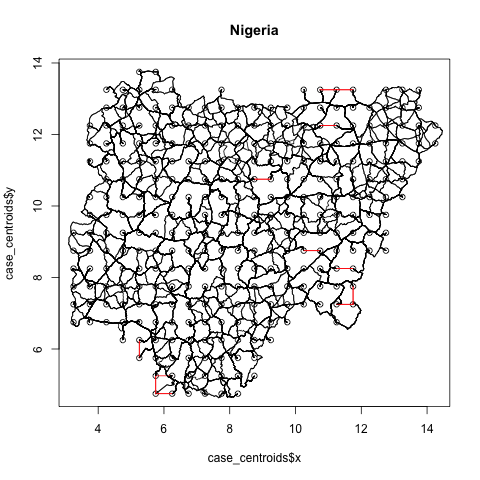
\includegraphics[width=\textwidth, trim={1cm 1cm 0cm 2cm},clip]{../../Build/output/Road_Networks/network_Nigeria.png}
\caption{Nigeria}
\label{fig:nigeria_roads}
\end{subfigure}
\begin{subfigure}[c]{0.43\textwidth}
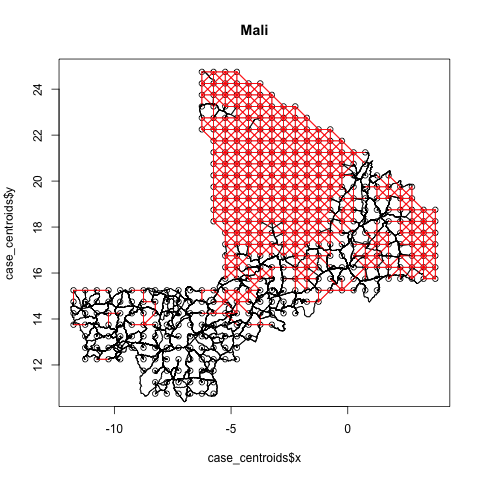
\includegraphics[width=\textwidth, trim={1cm 1cm 0cm 2cm},clip]{../../Build/output/Road_Networks/network_Mali.png}
\caption{Mali}
\label{fig:Mali_roads}
\end{subfigure}

\begin{subfigure}[c]{0.43\textwidth}
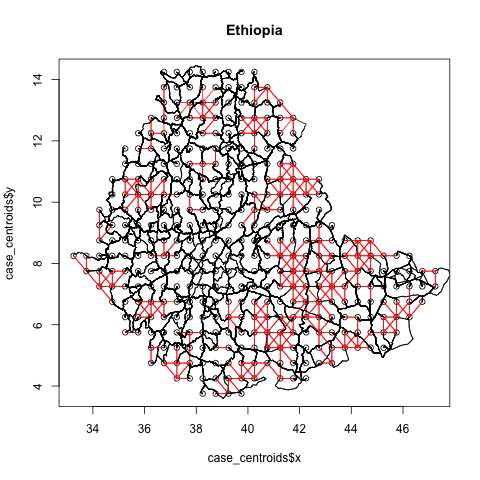
\includegraphics[width=\textwidth, trim={1cm 1cm 0cm 2cm},clip]{../../Build/output/Road_Networks/network_Ethiopia.png}
\caption{Ethiopia}
\label{fig:Ethiopia_roads}
\end{subfigure}
\begin{subfigure}[c]{0.43\textwidth}
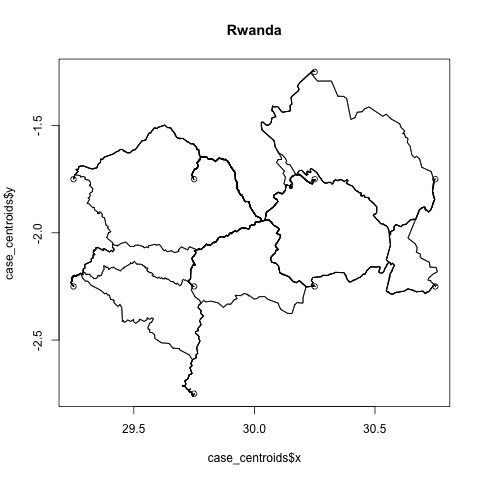
\includegraphics[width=\textwidth, trim={1cm 1cm 0cm 2cm},clip]{../../Build/output/Road_Networks/network_Rwanda.png}
\caption{Rwanda}
\label{fig:Rwanda_roads}
\end{subfigure}
\mysubcaption{Road Networks as scanned off Open Street Map (OSM). Black lines represent optimal routes from each grid cell centroid to each of its eight surrounding neighbours. These routes may include a portion walked by foot in order to get to the nearest street. Connections in which walking the entire distance is faster are printed as red straight lines. Axes denote degrees longitude (x) and latitude (y), respectively. Data scanned in November 2017.}

\label{fig:roads}
\end{figure}
% End Figure

The OSM routing algorithm is specified for cars and takes into account differential speeds attainable on different types of roads. However, if either start or destination location do not directly fall onto a street, the optimal route jumps to the nearest road and goes from there. To take this into account, I add a walking distance to the travel path. Agents are assumed to walk in straight lines to the nearest street at a fixed speed of 4 km/h. They then take the car and drive the route with average speed as specified by OSM, before they potentially have to walk the last stretch again to their exact centroid destination. For some particularly remote areas, even the nearest street is very far away, such that the car routing provided by OSM is not sensible. To counter these cases, I also calculate for all 70,000+ connections the outside option of walking the entire link in a straight line at 4 km/h. I then identify cases in which walking directly is actually faster than using OSM's proposed route (plus the travel to and from roads). In these cases, I replace OSM's route with the walking distance and constant 4 km/h speed.

Figure \ref{fig:roads} presents the resulting road networks for four countries. Figure \ref{fig:nigeria_roads} displays every optimal route for Nigeria, which appears overall fairly well connected. Commuters mostly seem to be able to drive relatively direct routes between locations, even though cases with substantial detours are also evident at second glance. Connections in which walking were the preferred alternative are displayed in red and fairly rare in Nigeria. Figure \ref{fig:Mali_roads} presents the case of Mali, which paints a different picture: for many connections through the Sahara desert in the north-east of the country, walking straight lines in the sand is actually the fastest way to get from A to B. Ethiopia in Figure \ref{fig:Ethiopia_roads} displays only a few trails connecting the country's east to the west. Small Rwanda in Figure \ref{fig:Rwanda_roads} zooms in on the actual roads taken and displays the intricacies of the optimal routing provided by OSM.

Relying on the open source community of OSM does come with some drawbacks. The most pressing concern is that data on the position and quality of roads are user-generated and hence subject to reporting bias. Richer areas may appear to be equipped with more roads if local residents have the time and necessary access to a computer to enter their neighbourhoods into the database. As soon as inference is conducted on the relationship between streets and any covariate of development, the resulting estimates will be biased. While this is certainly troubling, I believe this bias to be much more important on finer resolutions than the operating one in this study. Start and destination of the elicited routes are on average more than 55 kilometres apart and travel will hence take place mostly on larger roads and national highways. It is unlikely that these major streets are systematically underreported in OSM, the primary open source routing platform on the internet. It is nevertheless important to keep this potential flaw of the data in mind when conducting inference later on.\footnote{As this study merely pertains to within-country transport networks, I only look at connections between neighbouring locations of the same country. In some cases the optimal route between these locations might go through a neighbouring country. For instance, Senegal is effectively split into two parts by the intersecting country The Gambia. Still, when connecting Senegalese cell centroids just to the north and to the south of The Gambia (which are still less than 60km apart), the route will go over foreign soil. This presents a problem only in later policy recommendations, as political leaders of one country cannot necessarily legislate road improvements abroad. The rest of the analysis is not affected by this issue.} \footnote{In some rare cases (less than 0.1 per cent of all connections), the OSM algorithm cannot find any route between two neighbouring centroid locations. This is mostly due to an obvious geographic impossibility to connect two nodes. In Guinea-Bissau, for instance one location lies on the Bolama Islands just off the shore of mainland Guinea-Bissau. Its neighbouring locations are all on the mainland and hence unreachable by car. In other cases, both locations to be connected are in deep jungle or swampy regions. In all these cases, I treat the link as if the two locations were not neighbours in the first place. That implies I even forgo the backup possibility of walking the entire distance, assuming that agents cannot walk between islands or through the densest jungle.}

After having collected data on distance and average speed of the optimal route between all neighbouring centroid locations, the next step is to discretise these data in order to have a tractable network representation capable of performing the trade simulations necessary in the remainder of this study.

\subsubsection{Infrastructure Matrix \boldmath{$I_{i,k}$}}
To gain a conception of how much two nodes are connected in the transport network, I derive a numeric representation of how much \emph{current} infrastructure lies on the link between locations. In their own empirical analysis, \cite{Fajgelbaum_OptimalTransportNetworks_2017} use data on the average number on lanes of the streets used on a given route, and whether these streets are national or secondary roads. The OSM algorithm does not supply such detailed level of information for Africa. However, I argue that \citeauthor{Fajgelbaum_OptimalTransportNetworks_2017} are only proxying for a much more immediate statistic: the average speed with which one can travel on a given road. If two locations are linked by a faster connection, I assume this to be the result of higher infrastructure $I_{i,k}$ on this edge. I hence set
\begin{equation}
  I_{i,k} = \textrm{Average Speed}_{i,k}
\end{equation}

This measure is naturally bound from below at 4 km/h, as walking the air-line distance is always available as a backup. Empirically, average speeds range between 6 km/h (Mauritania, where most routes go through the desert and have to be covered by walking) and 33 km/h (Swaziland). It is the objective of the social planner to reduce trade costs between suitable trading partners by increasing the average speed $I_{i,k}$ with which transport can occur between them.

\subsubsection{Trade Cost Parameter \boldmath{$\delta_{i,k}^{\tau}$}}
Recall from equation \eqref{eq:tau} that iceberg trade costs between nodes $i$ and $k$ are modelled as $\tau_{i,k}^{n} = \delta^{\tau}_{i, k} \frac{(Q_{i,k}^{n})^{\beta}}{I_{i,k}^{\gamma}}$. Following \citeauthor{Fajgelbaum_OptimalTransportNetworks_2017} and ensuring convexity and strong duality, I parameterise $\beta = 1.245$ and $\gamma = 0.5\beta = 0.6225$.

$\delta^{\tau}_{i, k}$ is a scaling parameter. It impacts trade costs regardless of current infrastructure levels and congestion forces and hence allows for variation caused by exogeneous forces. To calibrate $\delta^{\tau}_{i, k}$, I make use of a recent contribution by \cite{Atkin_WhoGettingGlobalized_2015}. They use barcode-level data on sales prices of identical goods to back out trade costs between regions within both Nigeria and Ethiopia. They show that trade costs are significantly increasing in (log) distance between origin and destination, impeding much of mutually beneficial trade. Directly taking the average of their two point estimates for Ethiopia and Nigeria, I calculate
\begin{equation}
  \delta^{\tau}_{i,k} =  0.0466\times\textrm{ln}(\textrm{Distance}_{i,k})
  \label{eq:delta_tau}
\end{equation}

as the trade cost elasticity to distance travelled.\footnote{\citeauthor{Atkin_WhoGettingGlobalized_2015} (Table 2, page 44) estimate the coefficient as $0.0374$ for Ethiopia and $0.0558$ for Nigeria. My parameter is the simple average of these two point estimates.} Note that the functional form of \eqref{eq:tau} implies that the very first good to be shipped over a given link is free of any trade costs, with convex congestion forces coming into play only  afterwards. The social planner can invest into infrastructure along any link to attenuate these forces.

\subsubsection{Infrastructure Building Cost Matrix \boldmath{$\delta_{i,k}^{I}$}}
The \emph{Network Building Constraint} \eqref{eq:network_building} binds the social planner's action space when commissioning faster roads. Total cost of infrastructure $\sum_{i}^{}\sum_{k \in N(i)}^{} \delta_{i,k}^{I}I_{i,k}$ is fixed at $K$, which equals the cost of originally building the current network. In this set-up, $\delta_{i,k}^{I}$ denotes the relative constant cost of increasing the average speed on a given link by one. As $K$ is unrelated to the rest of the model it can be normalised to $K=1$ without loss of generality, so that only relative infrastructure building costs matter \citep{Fajgelbaum_OptimalTransportNetworks_2017}. This procedure allows me to stay agnostic about the actual (dollar-)cost of building roads and I only need to take a stance on which areas are cheaper or more expensive to build on \emph{relative to others}.

$\delta_{i,k}^{I}$ depends on a variety of inputs, like the distance of a road or the underlying terrain. I follow \citeauthor{Fajgelbaum_OptimalTransportNetworks_2017} who in turn make use of a recent study by \cite{Collier_CostRoadInfrastructure_2015}, which estimates infrastructure building costs in developing countries. Readily applying their specification, I calculate
\begin{equation}
  \textrm{ln}(\delta^{I}_{i,k,c}) = \delta_{c}^{I} - 0.11 \times \one_{\textrm{Distance}_{i,k,c} > 50km} + 0.12 \times \textrm{ln}(\textrm{Ruggedness}_{i,k,c}) + \textrm{ln}(\textrm{Distance}_{i,k,c})
  \label{eq:delta_I}
\end{equation}

as the constant cost of increasing infrastructure $I_{i,k}$ on the link between $i$ and $k$ in country $c$. $\textrm{Distance}_{i,k,c}$ denotes the road distance travelled between nodes and enters positively, implying that longer roads are costlier to develop as every single road kilometre will have to be improved. Moreover, the building cost per kilometre falls discretely when the distance surpasses 50 kilometres, as embodied by the indicator $\one_{\textrm{Distance}_{i,k,c} > 50km}$. Note that every route in my sample is longer than 50 kilometres and the corresponding dummy term is hence always equal to 1. $\textrm{Ruggedness}_{i,k,c}$ denotes the average ruggedness between grid cells $i$ and $k$ and enters positively, highlighting the additional expenses accompanied with building on uneven terrain.\footnote{Data on local ruggedness come from \cite{Henderson_GlobalSpatialDistribution_2018} and is described in more detail with other geographical covariates below.} $\delta_{c}^{I}$ is a country-specific scaling parameter. Its main purpose it to ensure that equation \eqref{eq:network_building} is satisfied with $K=1$. I first appraise the infrastructure network $I_{i,k}$ of all countries and then flexibly alter $\delta_{c}^{I}$ for each nation individually in order to comply with equation \eqref{eq:network_building}.

Note that $\textrm{Distance}_{i,k,c}$ denotes the distance travelled along the fastest route as described in section \ref{sec:road_data}, not the air-line distance between origin and destination centroid. This is significant in the sense that distance is treated as a primitive of the model and is not endogenously subject to the optimisation exercise. If under the current network two nodes are only connected via an extensive detour, the distance variable as reported by Open Street Map will be very large. The social planner is now merely equipped with the capacity to improve the infrastructure on the given route, but cannot devise an entirely new road shortcutting the detour. This restriction might very well be reasonable in certain situations. Some nodes might be only connected by circuitous routes because of major geographical obstacles like mountains or swamps between them. My conception of infrastructure investment ensures that no improbable road through a mountain is devised, but rather the path around the mountain is improved. On the other hand, my model might forgo obvious welfare-improving infrastructure projects based on entirely new roads. In the abstract formalism of the model, this distinction does not make that much of a difference. It can afford to stay ambiguous about whether trade costs are decreased by a new shortcut or by road improvements on the old connection. When using the predictions of the model to  inform actual transport policy, however, one has to bear in mind that entirely new roads might at times succeed in connecting regions at even lower costs than the improvements prescribed by my simulation.

\subsection{Heterogeneous Goods}
To build incentives for trade, I introduce $N=2$ different goods: an agricultural and an urban good. Since economic output is proxied by night luminosity, I cannot observe the distribution of different goods in a given grid cell, but only their total production. This leads to the total specialisation assumption outlined above in which urban grid cells are solely producing the urban good, while all other grid cells are producing nothing but the agricultural good.

To classify grid cells as urban or rural I use an iterative procedure, which seeks to match each country's 2016 urbanisation rate as reported by \cite{TheWorldBank_WorldBankAnnual_2017}. I start by assuming every location is a city and then gradually proceed to re-classify the least densely populated locations, until the ratio of people living in urban areas to total population equals that of the World Development Indicators.\footnote{For three countries, the WDI do not report urbanisation rates. In these cases, I match the overall urbanisation rate for the entire African continent of 42 per cent as reported by \cite{Lall_AfricaCitiesOpening_2017}.} With this procedure, seven per cent of grid cells are classified as urban. These cells inhabit 40 per cent of the continent's population, matching recent figures from \cite{Lall_AfricaCitiesOpening_2017} fairly well.

As discussed above, the model stays agnostic about how grid cells produce their luminosity output. The only assumption it makes is that cells can ever only produce one of the two varieties and their productivity in the respective other variety is zero. I thereby avoid having to divide total lights by total population in order to obtain total factor productivity, a procedure which has occasionally been used \citep[see e.g.][]{DeLuca_Ethnicfavoritismaxiom_2018}, even though the literature has recently moved towards a consensus of warning against it \citep{Michalopoulos_SpatialPatternsDevelopment_2018}.

\begin{figure}[t]
\centering
\caption{Discretised Networks for Different Countries}

\begin{subfigure}[c]{0.45\textwidth}
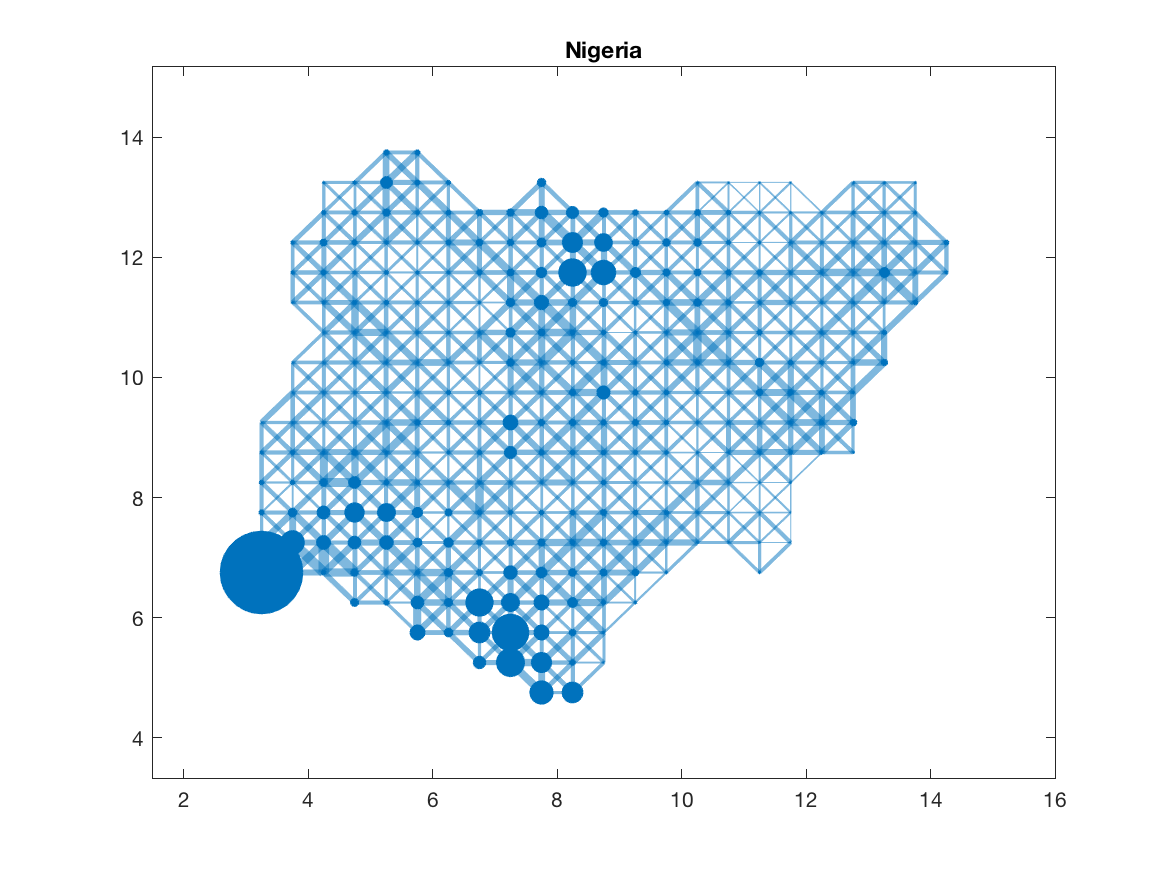
\includegraphics[width=\textwidth, trim={2cm 1cm 1.5cm 0cm},clip]{../../Build/output/Matlab_graphs/Nicer_graphs/Nigeria_stat.png}
\caption{Nigeria}
\label{fig:nigeria_mat}
\end{subfigure}
\begin{subfigure}[c]{0.45\textwidth}
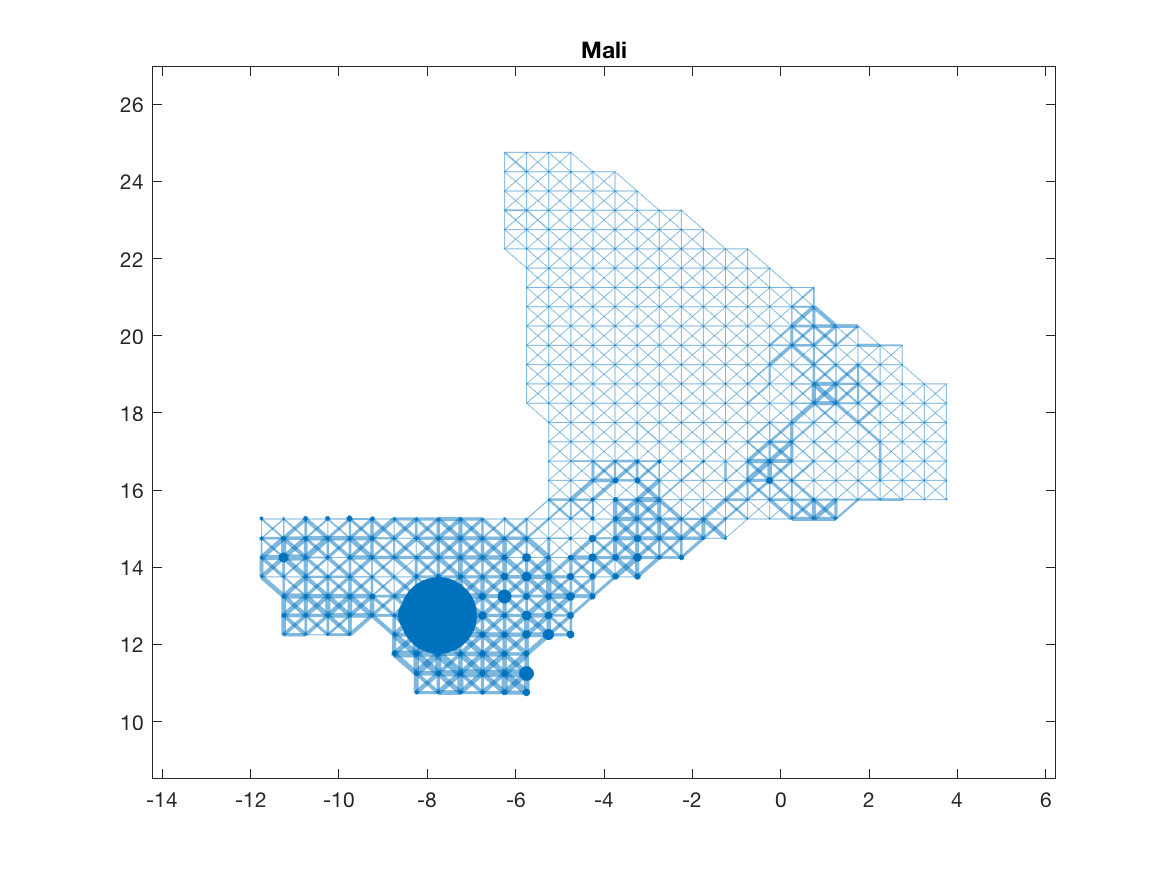
\includegraphics[width=\textwidth, trim={2cm 1cm 1.5cm 0cm},clip]{../../Build/output/Matlab_graphs/Nicer_graphs/Mali_stat.png}
\caption{Mali}
\label{fig:Mali_mat}
\end{subfigure}

\begin{subfigure}[c]{0.45\textwidth}
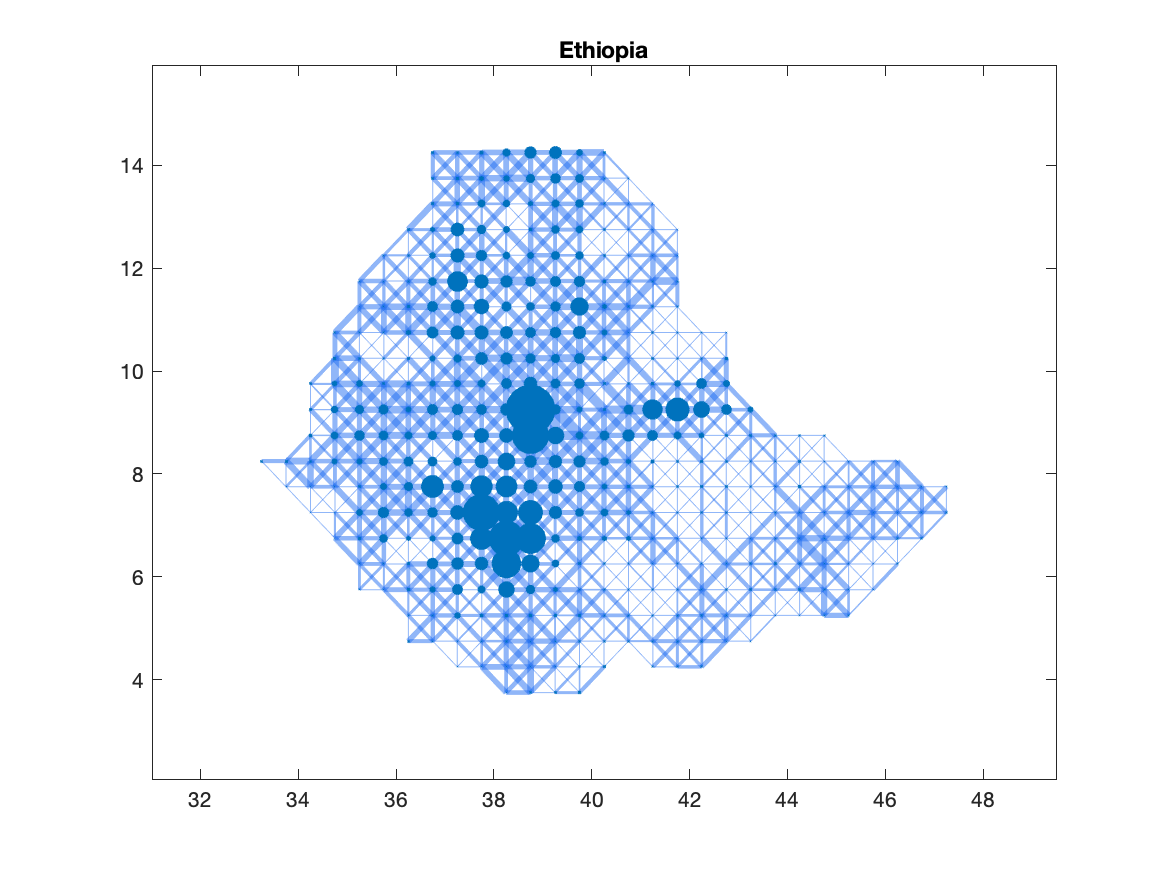
\includegraphics[width=\textwidth, trim={2cm 1cm 1.5cm 0cm},clip]{../../Build/output/Matlab_graphs/Nicer_graphs/Ethiopia_stat.png}
\caption{Ethiopia}
\label{fig:Ethiopia_mat}
\end{subfigure}
\begin{subfigure}[c]{0.45\textwidth}
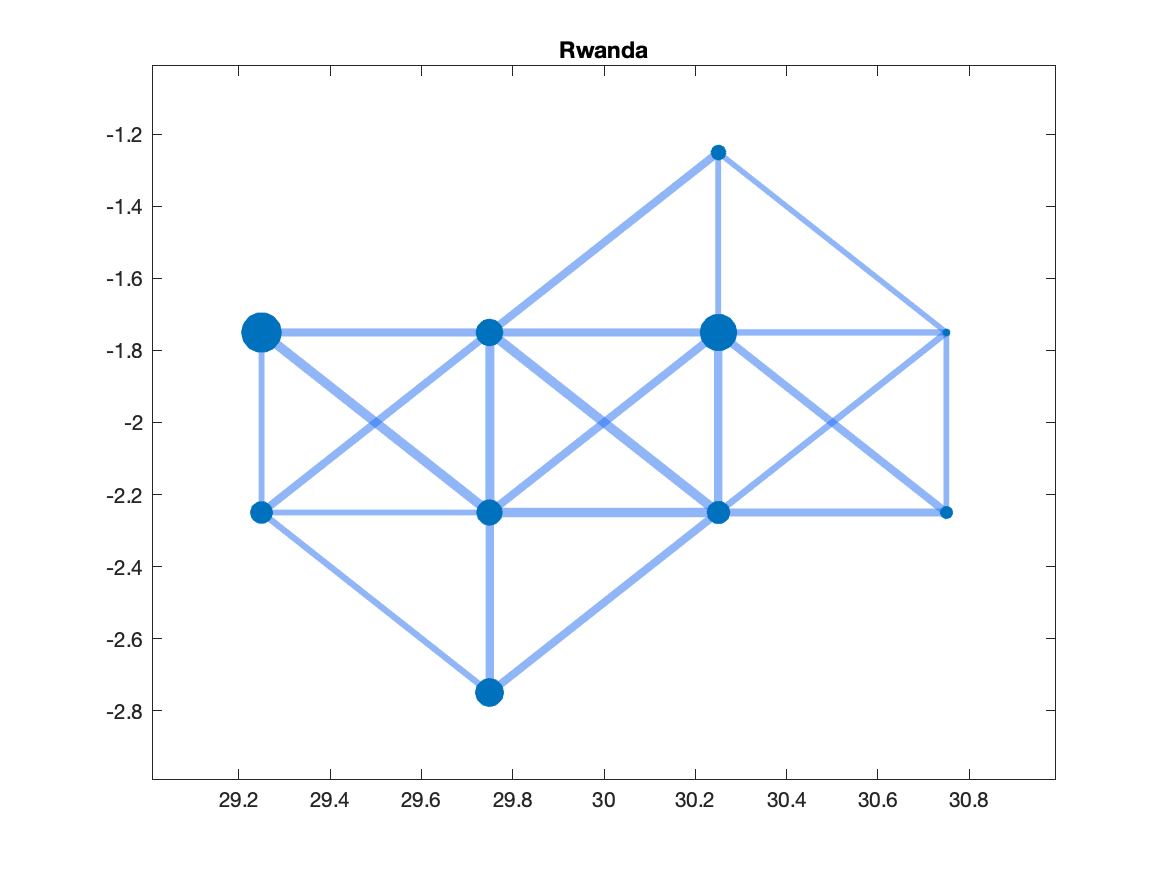
\includegraphics[width=\textwidth, trim={2cm 1cm 1.5cm 0cm},clip]{../../Build/output/Matlab_graphs/Nicer_graphs/Rwanda_stat.png}
\caption{Rwanda}
\label{fig:Rwanda_mat}
\end{subfigure}
\mysubcaption{Discretised representation of the infrastructure networks from Figure \ref{fig:roads}. Nodes are drawn with radius proportional to total population, edges' thickness correspond to average attainable speed on the route connecting the nodes.}
\label{fig:matlab_networks}
\end{figure}


\subsection{Simulation}

After these steps, a discretised network representation exists for every African country. Nodes in the network are the spaced centroid locations of each grid cell. They combine the characteristics of the entire grid cell (population, output, etc.) in one point. Edges in the network are road connections between centroids. Each edge also carries a number of characteristics (average speed, trade costs, and infrastructure building costs). Figure \ref{fig:matlab_networks} presents this discretised network representation for the four countries from above. Nodes are printed larger proportional to their population. Edges are drawn thicker proportional to the initial infrastructure investment.

For each country, I conduct two simulations. In both exercises, I calibrate the curvature parameter of the utility function at $\alpha = 0.4$ and the elasticity of substitution parameter at $\sigma=4$.\footnote{The parametrisation of $\alpha$ is identical in \cite{Fajgelbaum_OptimalTransportNetworks_2017}. They, however, calibrate elasticity of substitution at $\sigma=5$, so slightly higher than my parameter. \cite{Head_GravityEquationsWorkhorse_2014} review 32 related studies and find a mean parameter of $\sigma=4.51$. This average is driven by some positive outliers as the median parameter is much to the left of that. To account for this slant, I choose $\sigma=4$.} In the first simulation exercise, infrastructure $I_{i,k}$ is treated as fixed. This is to obtain a baseline estimate of the spatial variation of welfare in each country. Locations are still allowed to trade with each other, but only over the exogeneous current road network. Formally, this corresponds to solving a slightly truncated version of the social planner exercise from above, where $I_{i,k}$ is simply dropped from the planner's set of control variables and exogeneously set to the empirical infrastructure matrix $I_{i,k}^{\textrm{empirical}}$.\footnote{Recall that the optimal network allocation exercise nests the problem of solving for optimal trade flows. Hence, every other aspect of the model remains unaffected by fixing $I_{i,k}$. Trivially, this makes the \emph{Network Building Constraint} \eqref{eq:network_building} non-binding. The same outcome could be achieved at much higher computational costs by simply introducing an additional constraint $I_{i,k} = I_{i,k}^{\textrm{empirical}}$ to the social planner's problem.} By construction, the resulting solution will have two properties. Firstly, total output over the entire country will remain untouched. Inputs are not defined and hence do not shift to more productive regions. Indeed, any welfare gains will be attained solely by shipping the right mix of goods to the right regions. Secondly, labor immobility will leave welfare differences between regions as agents cannot simply move to more privileged cells. The social planner would like to overcome these differences, but is confronted with trade costs which might leave certain remote areas much worse off than well-connected ones.

Following this static exercise, I proceed to the main task of endogenizing the infrastructure matrix $I_{i,k}$. With the \emph{Network Building Constraint} binding total infrastructure investment at the level of the current road network, the social planner is now free to reshuffle roads within the country in order to improve connections as she chooses. If she wants to improve the connection between two given locations, she will have to take away infrastructure from somewhere else in the country. This reallocation exercise does not seek to identify where to place the optimal next investment, but rather represents an utterly fictitious scenario in which every road can be lifted from the ground, reshuffled, and eventually located someplace else.\footnote{Note that equation \eqref{eq:network_building} only fixes $\sum_{i}^{}\sum_{k \in N(i)}^{} \delta_{i,k}^{I}I_{i,k} = K$. Hence, not the overall sum of infrastructure is fixed, but more precisely the overall cost of infrastructure. This still allows the social planner to take away one unit of infrastructure on a very expensive (high $\delta_{i,k}^{I}$) link and exchange it for much more than one unit on a cheaper (low $\delta_{i,k}^{I}$) link.} The procedure does not measure how many roads a country has, but rather how well they are placed. It does not look at whether the entire country is full of speedy roads, but rather whether those roads connect the right locations.

I conduct the reallocation scenario for every African country. Six small countries (Cape Verde, Comoros, The Gambia, Mauritius, São Tomé and Príncipe, and Reunion) are too small to form a sensible network as they only show up as a single location in the dataset and are henceforth no longer considered. Computation times are greatly diminished when exploiting the strong convexity of the optimisation setting and solving the dual problem as sketched in the technical appendix of \cite{Fajgelbaum_OptimalTransportNetworks_2017}. Optimisations are performed via \textsc{Matlab}'s \texttt{fmincon} command. When conducting the simulations, I bind the social planner's set of permissible roads from below, at 4 km/h (such that $I_{i,k} \geq 4$ $ \forall \textrm{ } i \in \mathcal{I},k \in N(i)$). This is motivated by the assumption at the beginning that walking straight lines at this speed is conceived as an outside option and always available to any commuter. The social planner should not be able to force commuters to travel slower than walking in order to build a faster road elsewhere.\footnote{Contrarily, I do not explicitly restrict possible investments from above (at least not in addition to the sum-restriction imposed by Equation \ref{eq:network_building}), as this could violate the strong convexity of the problem. Not bounding the problem in principle allows the social planner to combine every available infrastructure from all over the country into one supersonic speed highway on one particular edge. However, the model is calibrated in a way which makes this very unattractive to the planner anyway. After simulating reallocation in every African country, less than 0.8\% of all 70,000+ built roads were suggested to be over 260 km/h. Still, one outlier of 2007 km/h (in Egypt) and one of 1755 km/h (in South Africa) remain.}

\afterpage{
\vfill
\begin{figure}[]
\centering
\caption{Reallocation Scenario for Different Countries}

\begin{subfigure}[c]{0.45\textwidth}
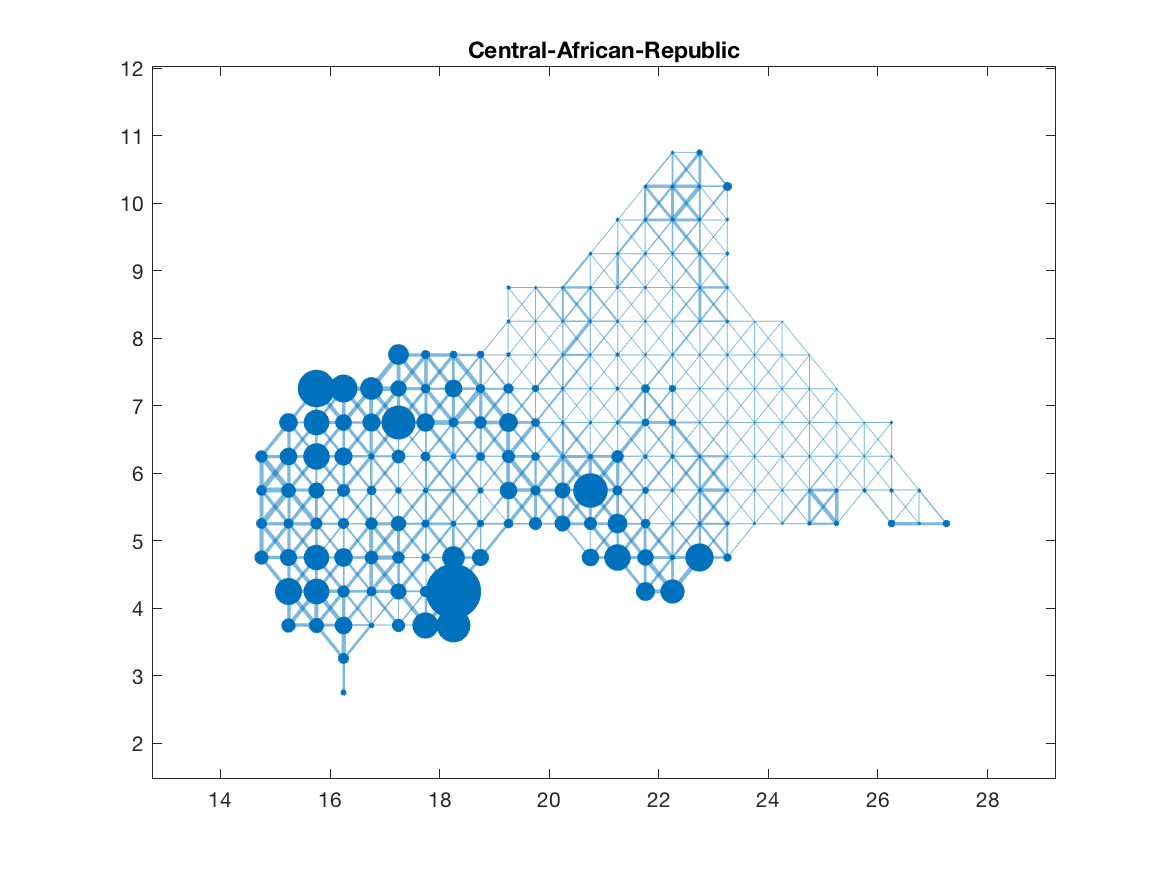
\includegraphics[width=\textwidth, trim={2cm 1cm 1.5cm 0cm},clip]{../../Build/output/Matlab_graphs/Nicer_graphs/Central-African-Republic_stat.png}
\caption{Central African Republic, pre reallocation}
\label{fig:cae_pre}
\end{subfigure}
\begin{subfigure}[c]{0.45\textwidth}
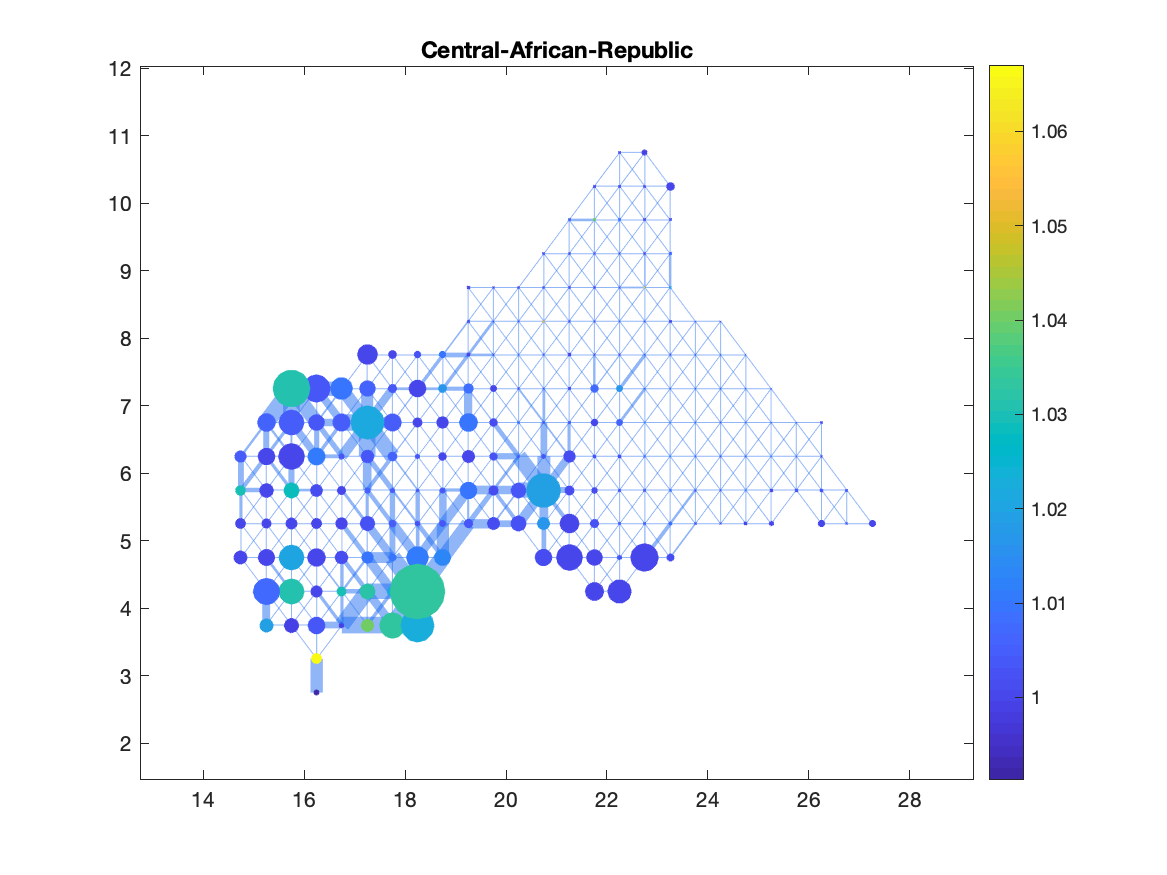
\includegraphics[width=\textwidth, trim={2cm 1cm 1.5cm 0cm},clip]{../../Build/output/Matlab_graphs/Nicer_graphs/Central-African-Republic_opt.png}
\caption{Central African Republic, post reallocation}
\label{fig:cae_post}
\end{subfigure}

\begin{subfigure}[c]{0.45\textwidth}
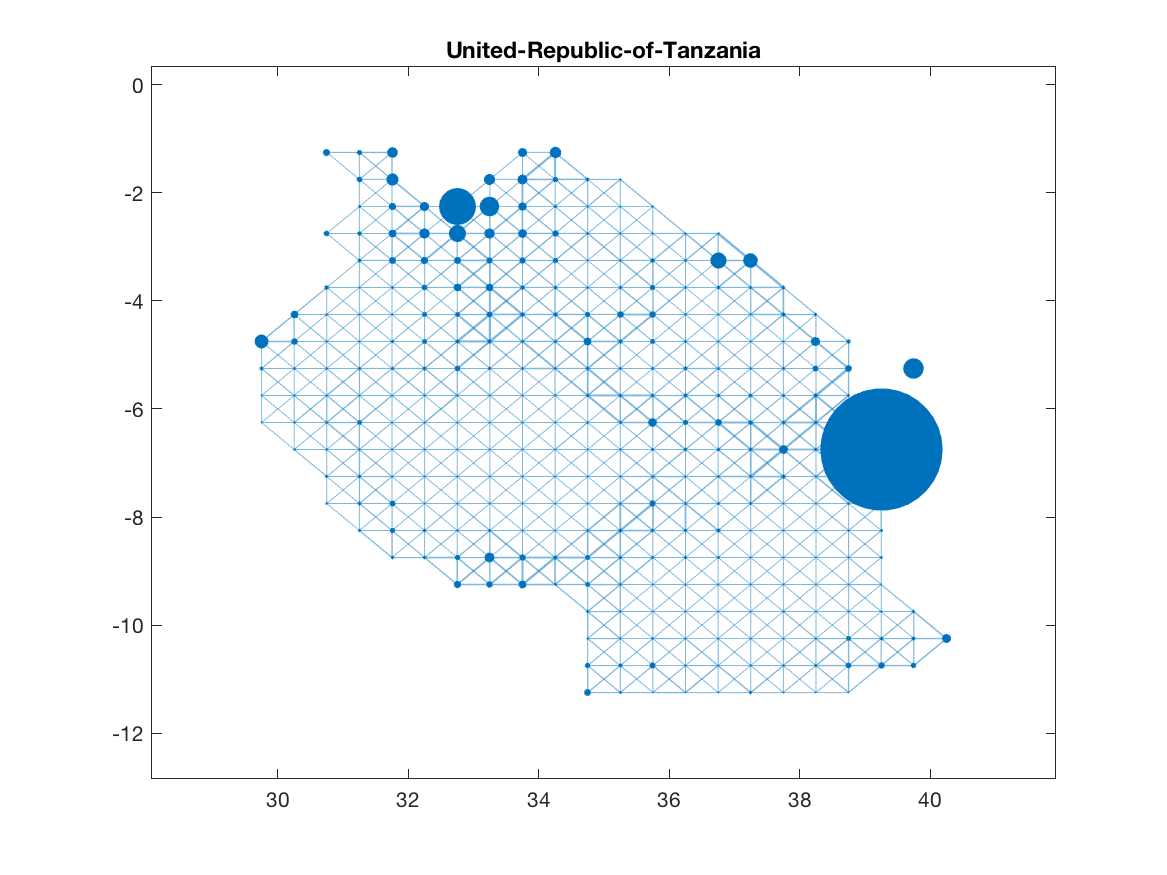
\includegraphics[width=\textwidth, trim={2cm 1cm 1.5cm 0cm},clip]{../../Build/output/Matlab_graphs/Nicer_graphs/United-Republic-of-Tanzania_stat.png}
\caption{Tanzania, pre reallocation}
\label{fig:tanzania_pre}
\end{subfigure}
\begin{subfigure}[c]{0.45\textwidth}
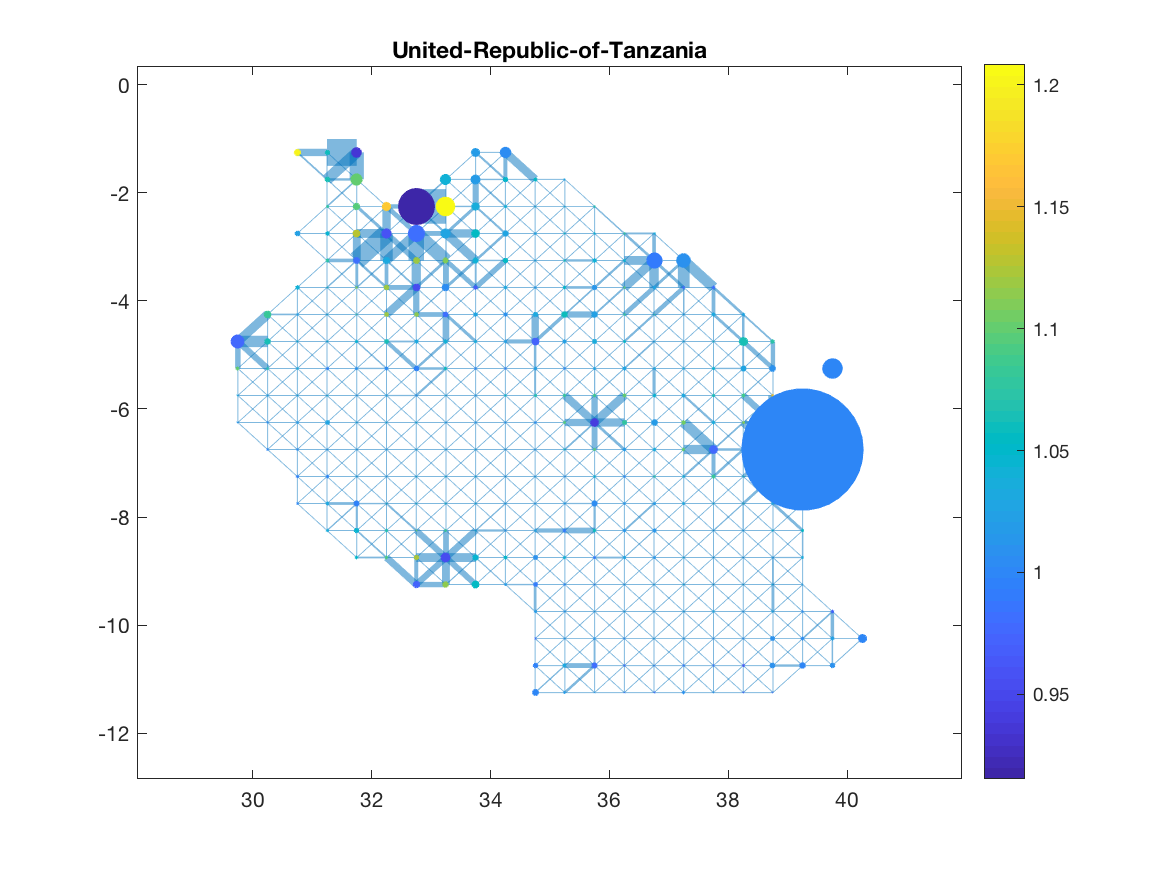
\includegraphics[width=\textwidth, trim={2cm 1cm 1.5cm 0cm},clip]{../../Build/output/Matlab_graphs/Nicer_graphs/United-Republic-of-Tanzania_opt.png}
\caption{Tanzania, post reallocation}
\label{fig:tanzania_post}
\end{subfigure}

\begin{subfigure}[c]{0.45\textwidth}
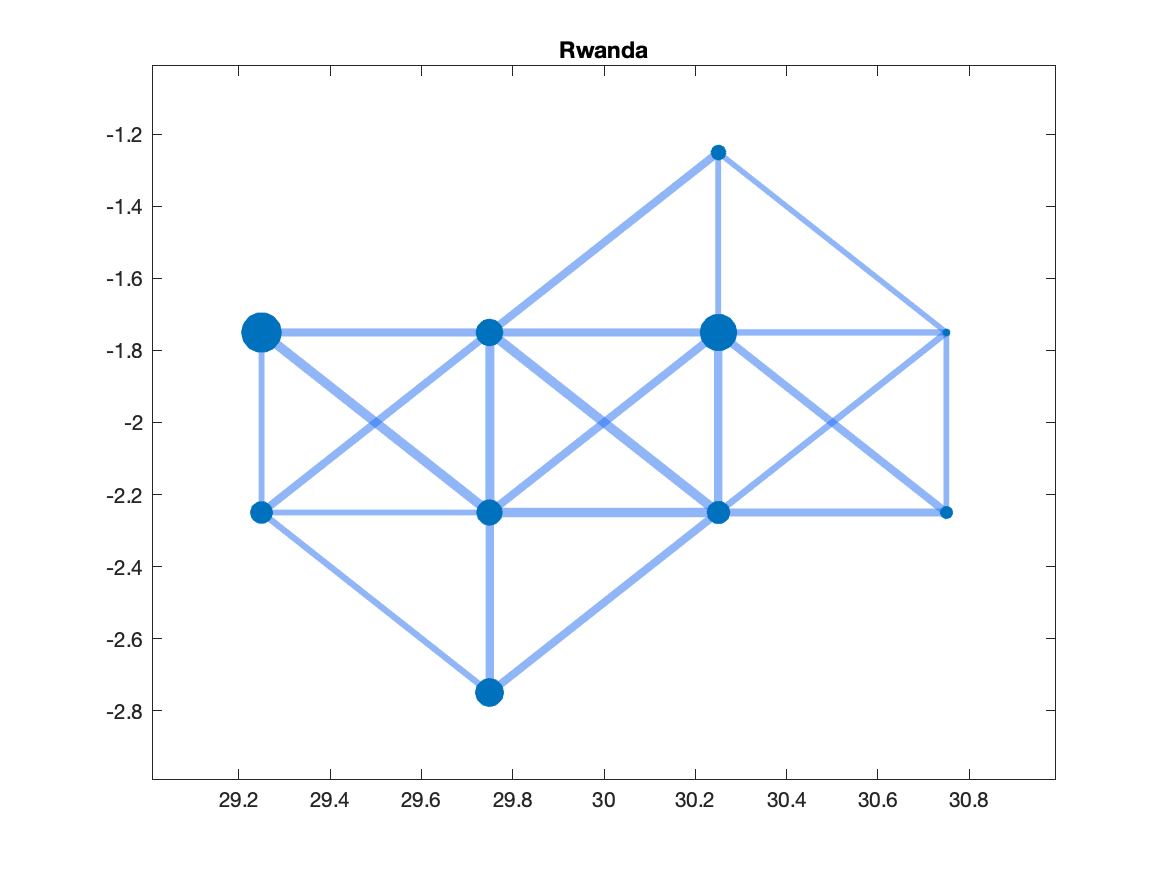
\includegraphics[width=\textwidth, trim={2cm 0cm 1.5cm 0cm},clip]{../../Build/output/Matlab_graphs/Nicer_graphs/Rwanda_stat.png}
\caption{Rwanda, pre reallocation}
\label{fig:rwanda_pre}
\end{subfigure}
\begin{subfigure}[c]{0.45\textwidth}
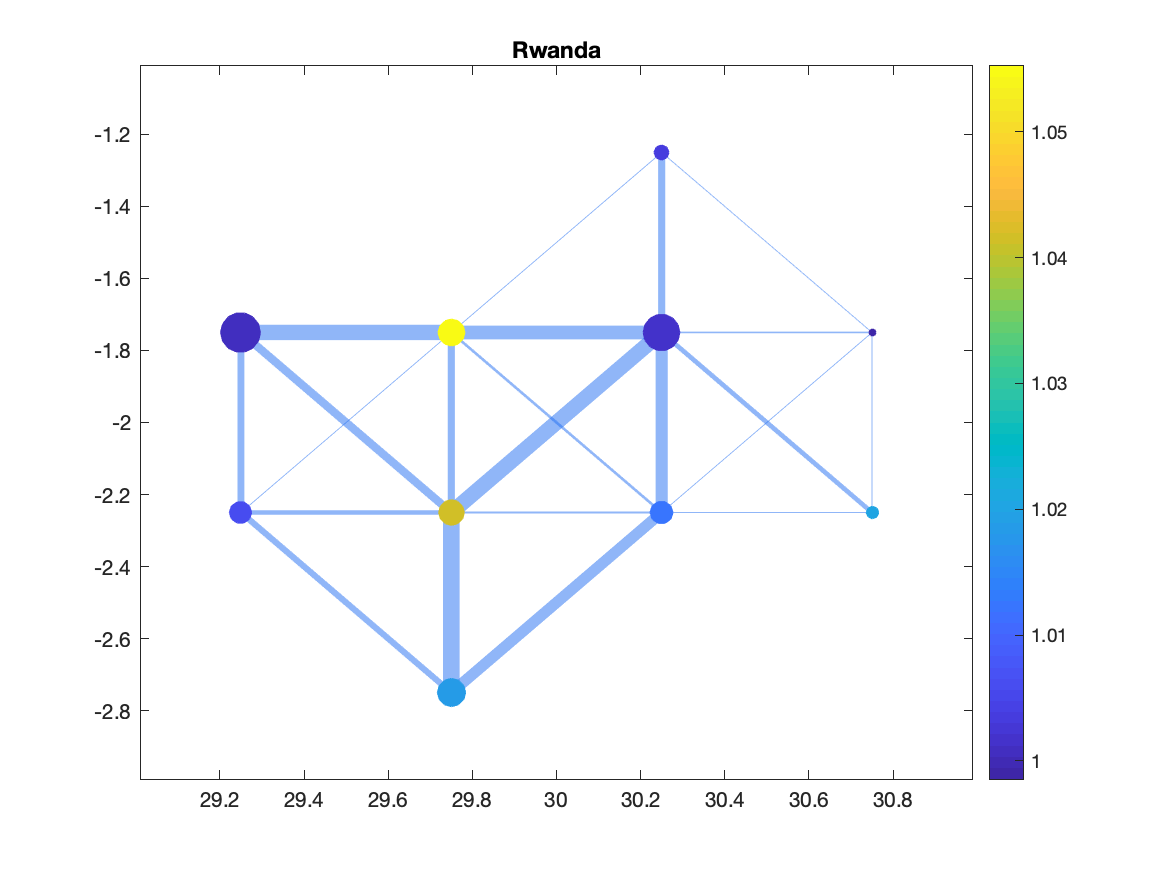
\includegraphics[width=\textwidth, trim={2cm 0cm 1.5cm 0cm},clip]{../../Build/output/Matlab_graphs/Nicer_graphs/Rwanda_opt.png}
\caption{Rwanda, post reallocation}
\label{fig:rwanda_post}
\end{subfigure}

\mysubcaption{Results from optimally reshuffling roads in three African countries. In each network graph, every node represents a grid cell centroid location with radius proportional to the size of its local population. Edges are drawn thicker depending on their allotted infrastructure $I_{i,k}$ (i.e. average attainable speed). In the optimal networks on the right, nodes are coloured based on their relative welfare gains and losses. Note the slightly different color scales for each country.}
\label{fig:Reallocations}
\end{figure}
\vfill
\clearpage
}
Figure \ref{fig:Reallocations} visualises this reallocation exercise for several countries. Subfigure \ref{fig:cae_pre} displays the discretised network representation of the Central African Republic, comparable to Figures \ref{fig:nigeria_mat} -- \ref{fig:Rwanda_mat}. The edges to this network are printed almost evenly thick, implying that infrastructure is fairly evenly distributed across the country. Subfigure \ref{fig:cae_post} then displays the country after the network reshuffling exercise. Three patterns stand out. First, the social planner sees a clear need to connect the populous areas in the south-west of the country with each other. Some southern nodes are granted extensive, almost highway-like connections to their immediate neighbours. For that, the social planner is willing to salvage some of the apparently unnecessary infrastructure in the middle or north of the country. Second, there still is a benefit to having a few trails connecting the south-west with the north-east. Some clear north-south and east-west routes spanning multiple regions emerge. Thirdly, nodes are printed in a colour scale corresponding to individual welfare gains and losses for each location. As can be seen from first-glance, most southern regions stand to gain between five and ten per cent of total welfare from this scenario. Hardly any nodes seem to lose welfare, even though on second glance a few instances become apparent.

Tanzania in Figures \ref{fig:tanzania_pre} -- \ref{fig:tanzania_post} displays a more decentralised optimal network solution. The reallocation scenario results in the main urban areas being better connected to their immediate surroundings, but no clear overarching network emerges. There also does not appear to be any necessity to better connect hinterland regions with the primal city Dar es Salaam in the east. Indeed, the largest city slightly loses welfare with the reallocation at the expense of multiple smaller population centres in the north.\footnote{On a side note, Tanzania also illustrates an interesting case where a tiny fraction of the country is fully detached from the rest of the network. Just north of Dar es Salaam, the island of Zanzibar constitutes a one-node subnetwork of its own. Not surprisingly, it remains completely unaffected by the reshuffling of roads on the mainland. Instances like these are relatively common in the dataset.} Small Rwanda in Figures \ref{fig:rwanda_pre} -- \ref{fig:rwanda_post} helps to illustrate some of the forces at hand in a less crowded graph. Starting from a fairly evenly distributed transport network, the reallocation dynamics lead to much more variation in infrastructure provision. Some links are deemed superfluous and hence reduced to the smallest admissible level, while others are scaled to multiple times their starting infrastructure stock. Furthermore, high welfare gains are reported by direct neighbours of big production centres and urban grid cells. These are unassuming grid cells with average population or output levels, merely equipped with the geographical blessing of being close to a bigger neighbour. This leads to the conclusion that while better infrastructure combats the welfare costs of geographical distance, proximity to hubs still matters. Even an optimally designed transport network is ultimately not able to fully overcome the \emph{curse of distance}.\footnote{A term coined by \cite{Boulhol_Havedevelopedcountries_2010}.}

The optimisation exercise pertains to regional goods trade over an internal geography of African countries. In this, it necessarily abstracts from other forces shaping the design of national transport networks. Firstly, my model does not feature human travel. Infrastructure is allocated with the sole aim of streamlining the flow of goods between regions. In reality, however, one of the main motivations for connecting places is facilitating the travel of people between them. My model ignores this factor. Secondly, patterns in regional goods flows might be driven by external forces outside a country's immediate economic topography. In considering closed economies, my model might overlook that some regions are extraordinarily well connected because they are important export hubs from which goods leave for the rest of the world. Similarly, regions close to national borders might be more economically affected by gravitational forces from large trade hubs on the other side of the border. My model does not consider any open economy effects. In my empirical investigation below, I employ a variety of control variables to account for these confounds -- for now, it is important to merely be aware of these limits to my model.

After successfully reshuffling a country's transport network, overall welfare will necessarily (weakly) increase. It is the social planner's objective to maximise overall welfare, and since the original network composition is always still available, the entire country cannot on aggregate be worse off than before. Note again that overall production (light output) will be unaffected by the entire exercise. Welfare gains are solely caused by enabling mutual benefits from trade through connecting the right locations. Nevertheless, they are substantial. The Central African Republic of Figure \ref{fig:Reallocations}, for instance, stands to gain 1.84\% of overall welfare just by reshuffling its roads. Tanzania (1.7\%) and Rwanda (1.27\%) are slightly closer to their hypothetical optimum.

\begin{figure}
\centering
\caption{African Countries by Network Inefficiency}
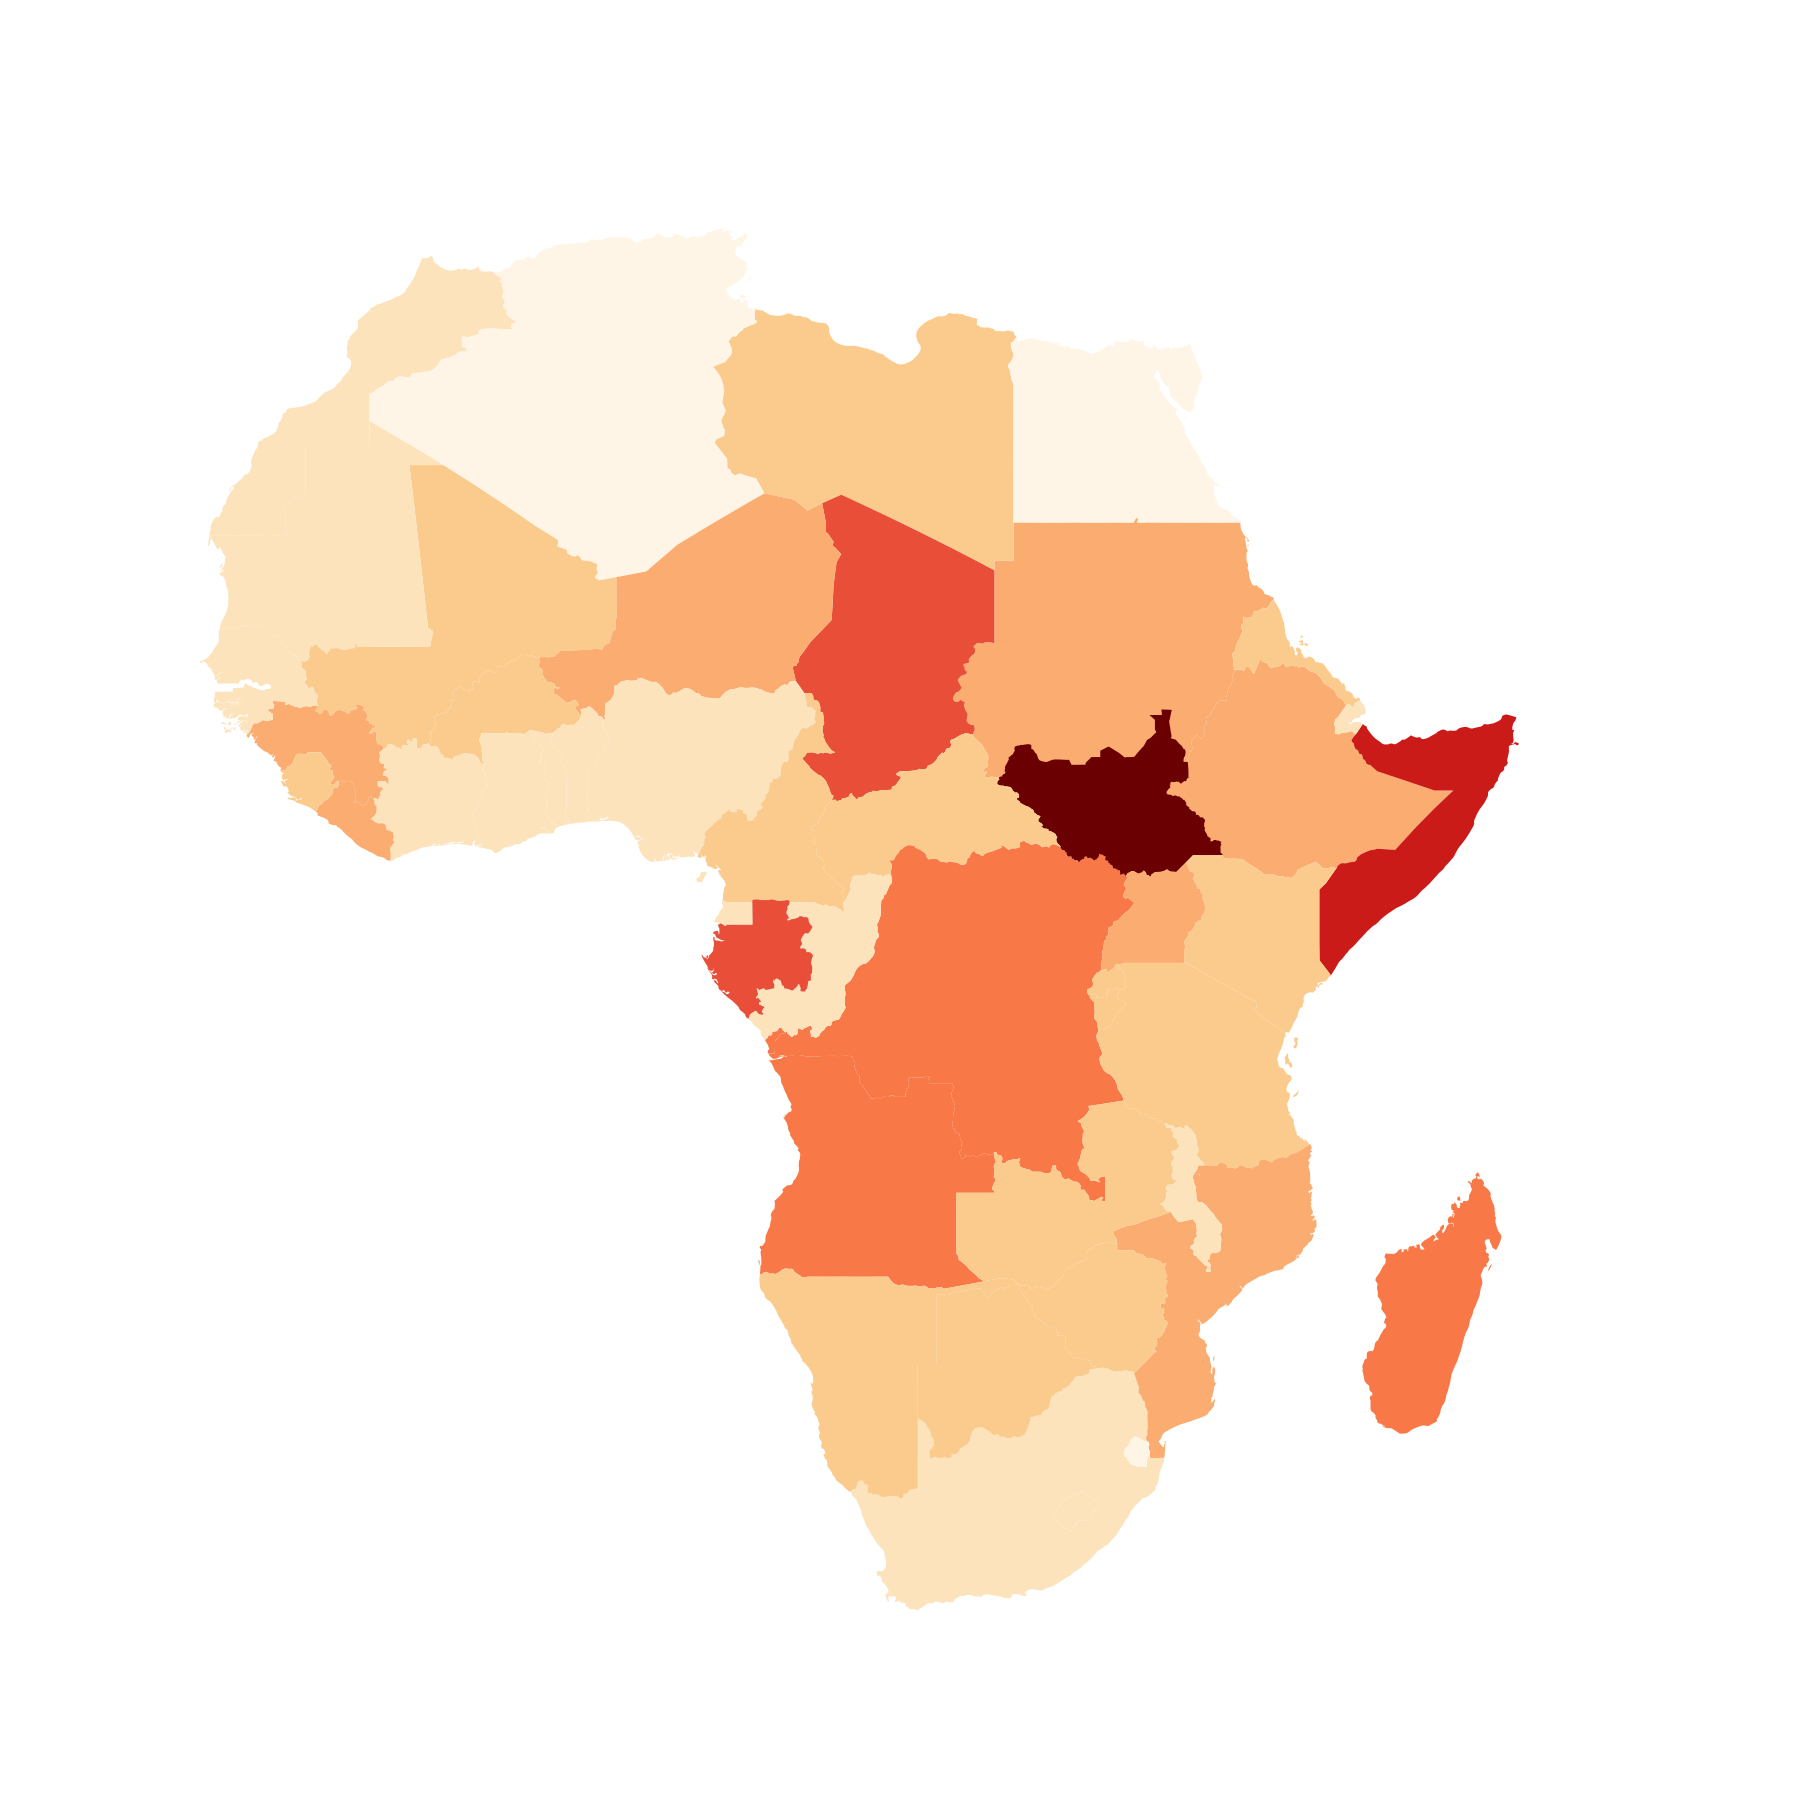
\includegraphics[width=0.6\textwidth,trim={1cm 4cm 1cm 3cm},clip]{../../Analysis/output/zeta_heatmaps/African_countries_zeta.png}

\label{fig:countries_by_welfare_gain}
\mysubcaption{Countries coloured according to their welfare gain under the optimal reallocation counterfactual. Scale from almost 7\% (dark red) to $<1\%$ (white) welfare gains. Gains are computed by comparing the population-weighted sum of utility levels over all grid cells in a country before and after the reallocation exercise.}
\end{figure}

Figure \ref{fig:countries_by_welfare_gain} displays all African countries and their hypothetical welfare gain. The three countries from above perform rather well in comparison. Some (mostly more developed) nations like South Africa (0.5\% welfare gains) or Tunisia (0.2\%) perform even better. Many countries are leaving much more on the table, like Somalia (4.8\%) or Chad (4.3\%). No African country, however, has a more ill advised road network than South Sudan. Its citizens stand to gain almost 6.7\% of overall welfare if just their roads were better placed. This might not come as a surprise, as the world's newest country has largely inherited a road network that was not conceived to sustain an independent nation, but rather connect it to its former capital up north. For the entire continent, optimal reallocation of national road systems would improve overall welfare by 1.15\%.

Forgone welfare gains can be conceived as an intuitive measure for overall network inefficiency. The closer hypothetical gains to zero (the lighter the country's colour), the more efficient the current allocation of roads. Vice-versa, if a country stands to gain a lot from reshuffling, then the current network is deemed more inefficient. On a simple cross-section, countries with less efficient networks are significantly correlated with more corruption ($p < 0.01$), less property rights ($p < 0.01$) and less 2010 log GDP ($p=0.07$). Note that these are merely descriptive correlations which are far from implying any form of causation.\footnote{Data from \cite{TheWorldBank_WorldBankAnnual_2017}. For corruption and property rights, data are only available for 35 countries and correlations are hence performed on this truncated sample. Interestingly, network efficiency is \emph{not} statistically associated with earlier independence years ($p=0.8$) or more artificial border designs ($p=0.3$) as reported by \cite{Alesina_ArtificialStates_2011}.}

While each country only stands to gain overall welfare from the reallocation procedure, individual locations might very well lose in the process. Intuitively, some regions might be equipped with far too many good roads such that the social planner takes these roads away to use someplace else. Comparing each grid cell's welfare before and after the major reshuffling can help to identify regions which are currently over or underprovided for. More formally, I define

\begin{equation}
  \Lambda_{i} = \frac{\textrm{Welfare under the optimal Infrastructure}_{i}}{\textrm{Welfare under the current Infrastructure}_{i}}
\end{equation}

% Figure
\begin{figure}[t]
\centering
\caption{Spatial Distribution of $\Lambda_{i}$ for Sample Countries}

\begin{subfigure}[c]{0.32\textwidth}
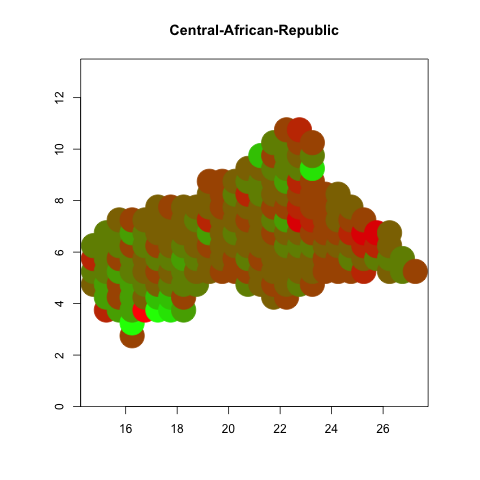
\includegraphics[width=\textwidth]{../../Analysis/output/zeta_heatmaps/Central-African-Republic_zeta.png}
\caption{Central African Republic}
\label{fig:Central African Republic_zeta}
\end{subfigure}
\begin{subfigure}[c]{0.32\textwidth}
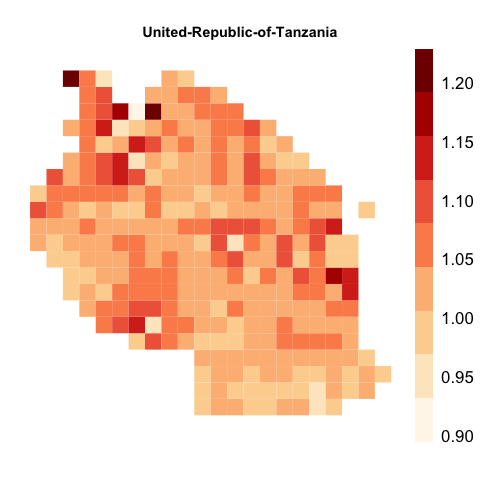
\includegraphics[width=\textwidth]{../../Analysis/output/zeta_heatmaps/United-Republic-of-Tanzania_zeta.png}
\caption{Tanzania}
\label{fig:Tanzania_zeta}
\end{subfigure}
\begin{subfigure}[c]{0.32\textwidth}
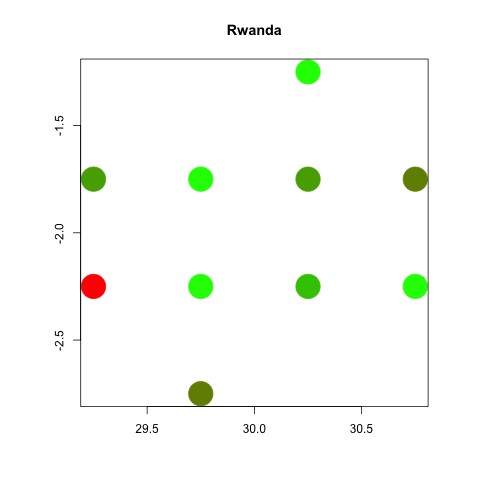
\includegraphics[width=\textwidth]{../../Analysis/output/zeta_heatmaps/Rwanda_zeta.png}
\caption{Rwanda}
\label{fig:Rwanda_zeta}
\end{subfigure}

\begin{subfigure}[c]{0.32\textwidth}
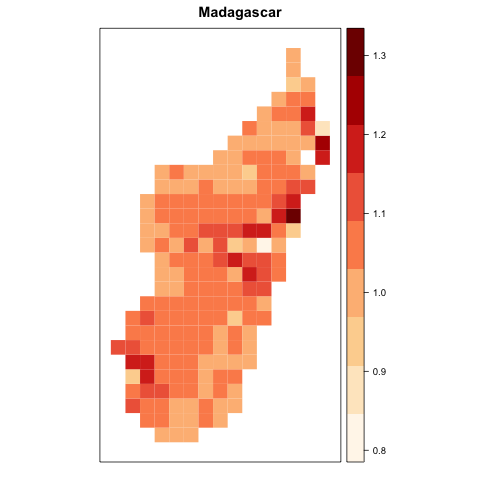
\includegraphics[width=\textwidth]{../../Analysis/output/zeta_heatmaps/Madagascar_zeta.png}
\caption{Madagascar}
\label{fig:Madagascar_zeta}
\end{subfigure}
\begin{subfigure}[c]{0.32\textwidth}
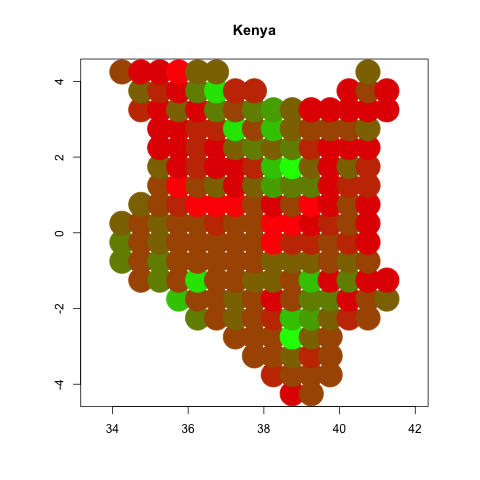
\includegraphics[width=\textwidth]{../../Analysis/output/zeta_heatmaps/Kenya_zeta.png}
\caption{Kenya}
\label{fig:Kenya_zeta}
\end{subfigure}
\begin{subfigure}[c]{0.32\textwidth}
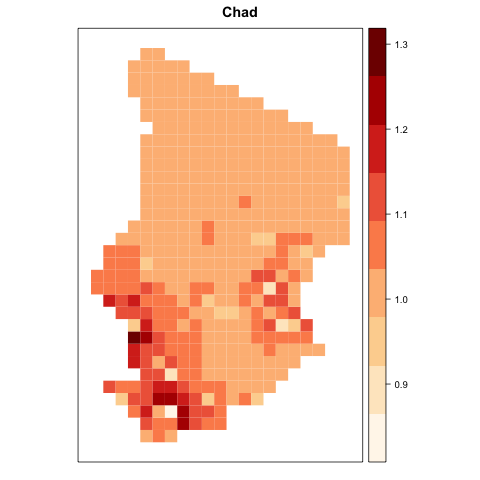
\includegraphics[width=\textwidth]{../../Analysis/output/zeta_heatmaps/Chad_zeta.png}
\caption{Chad}
\label{fig:Chad_zeta}
\end{subfigure}



\label{fig:zeta_countries}
\mysubcaption{Six African countries by their Local Infrastructure Discrimination Index $\Lambda_{i}$ on the grid cell level. Maps show each country as the 0.5 $\times$ 0.5 degree grid used for the network optimisation. For each map, darker shaded cells correspond to higher $\Lambda_{i}$ levels and hence more infrastructure discrimination compared to the optimal network. To better visualise within-country variation, colour scale slightly changes from country to country.}
\end{figure}
% End Figure

as the \emph{Local Infrastructure Discrimination Index} for grid cell $i$. Areas with high $\Lambda_{i}$ scores ($\Lambda_{i} > 1$) would be gaining under the optimal reallocation scenario and are hence under provided for in the network's current state. A score of $\Lambda_{i} < 1$ on the other hand, implies that a region is \emph{too} well off given its position in the network today and hence should be stripped off some of its infrastructure to increase overall welfare. Figure \ref{fig:zeta_countries} displays the spatial distribution of $\Lambda_{i}$ for six countries. The darker a grid cell's shade, the more it is disadvantaged by the inefficiencies of the current network. Figures \ref{fig:Central African Republic_zeta} -- \ref{fig:Rwanda_zeta} display what could already be inferred from the colouring of the nodes in Figure \ref{fig:Reallocations}: The Central African Republic has not enough fast roads in the south-west and too many in the east, Tanzania shows no clear spatial pattern, and Rwanda only engages in minor reshuffling. In Figures \ref{fig:Madagascar_zeta} -- \ref{fig:Chad_zeta} it, furthermore, becomes apparent that Madagascar's infrastructure network discriminates against the island's heartland (note how the coastal areas tend to be much lighter than the hinterland), Kenya would profit from connecting Nairobi to its surroundings, and Chad's south is discriminated against compared to the north.

In interpreting $\Lambda_{i}$, keep in mind that this is a measure of differences in \emph{welfare}. In this, it need not be a direct mapping of changes in actual infrastructure provision. Indeed, the highly non-linear nature of the optimal reallocation scenario can lead to situations in which a certain region substantially profits from the optimal policy, even though it is not directly granted additional roads. Local changes in welfare can instead be caused also by fortuitous peculiarities of geography -- maybe a neighbouring region emerges as a local trade hub, or the optimal network leads to improvements in the variety of goods, all without directly targeting each individual grid cell with additional roads. In my full dataset, changes in welfare $\Lambda_{i}$ are positively correlated with changes in infrastructure, yet the opposite is also true for some outliers.\footnote{Infrastructure changes computed as $^{\sum_{k \in N(i)}^{}I_{i,k}^{\textrm{opt}}} / _{\sum_{k \in N(i)}^{}I_{i,k}^{\textrm{empirical}}}$ correlate with $\Lambda_{i}$ at $p < 0.01$} In the remainder of this study, I will refer to high $\Lambda_{i}$ values as implying that a region is being awarded additional infrastructure from the social planner, even though the two need not necessarily be always equivalent.

% Figure
\begin{figure}
\centering
\caption{Spatial Distribution of $\Lambda_{i}$ for Entire Sample}
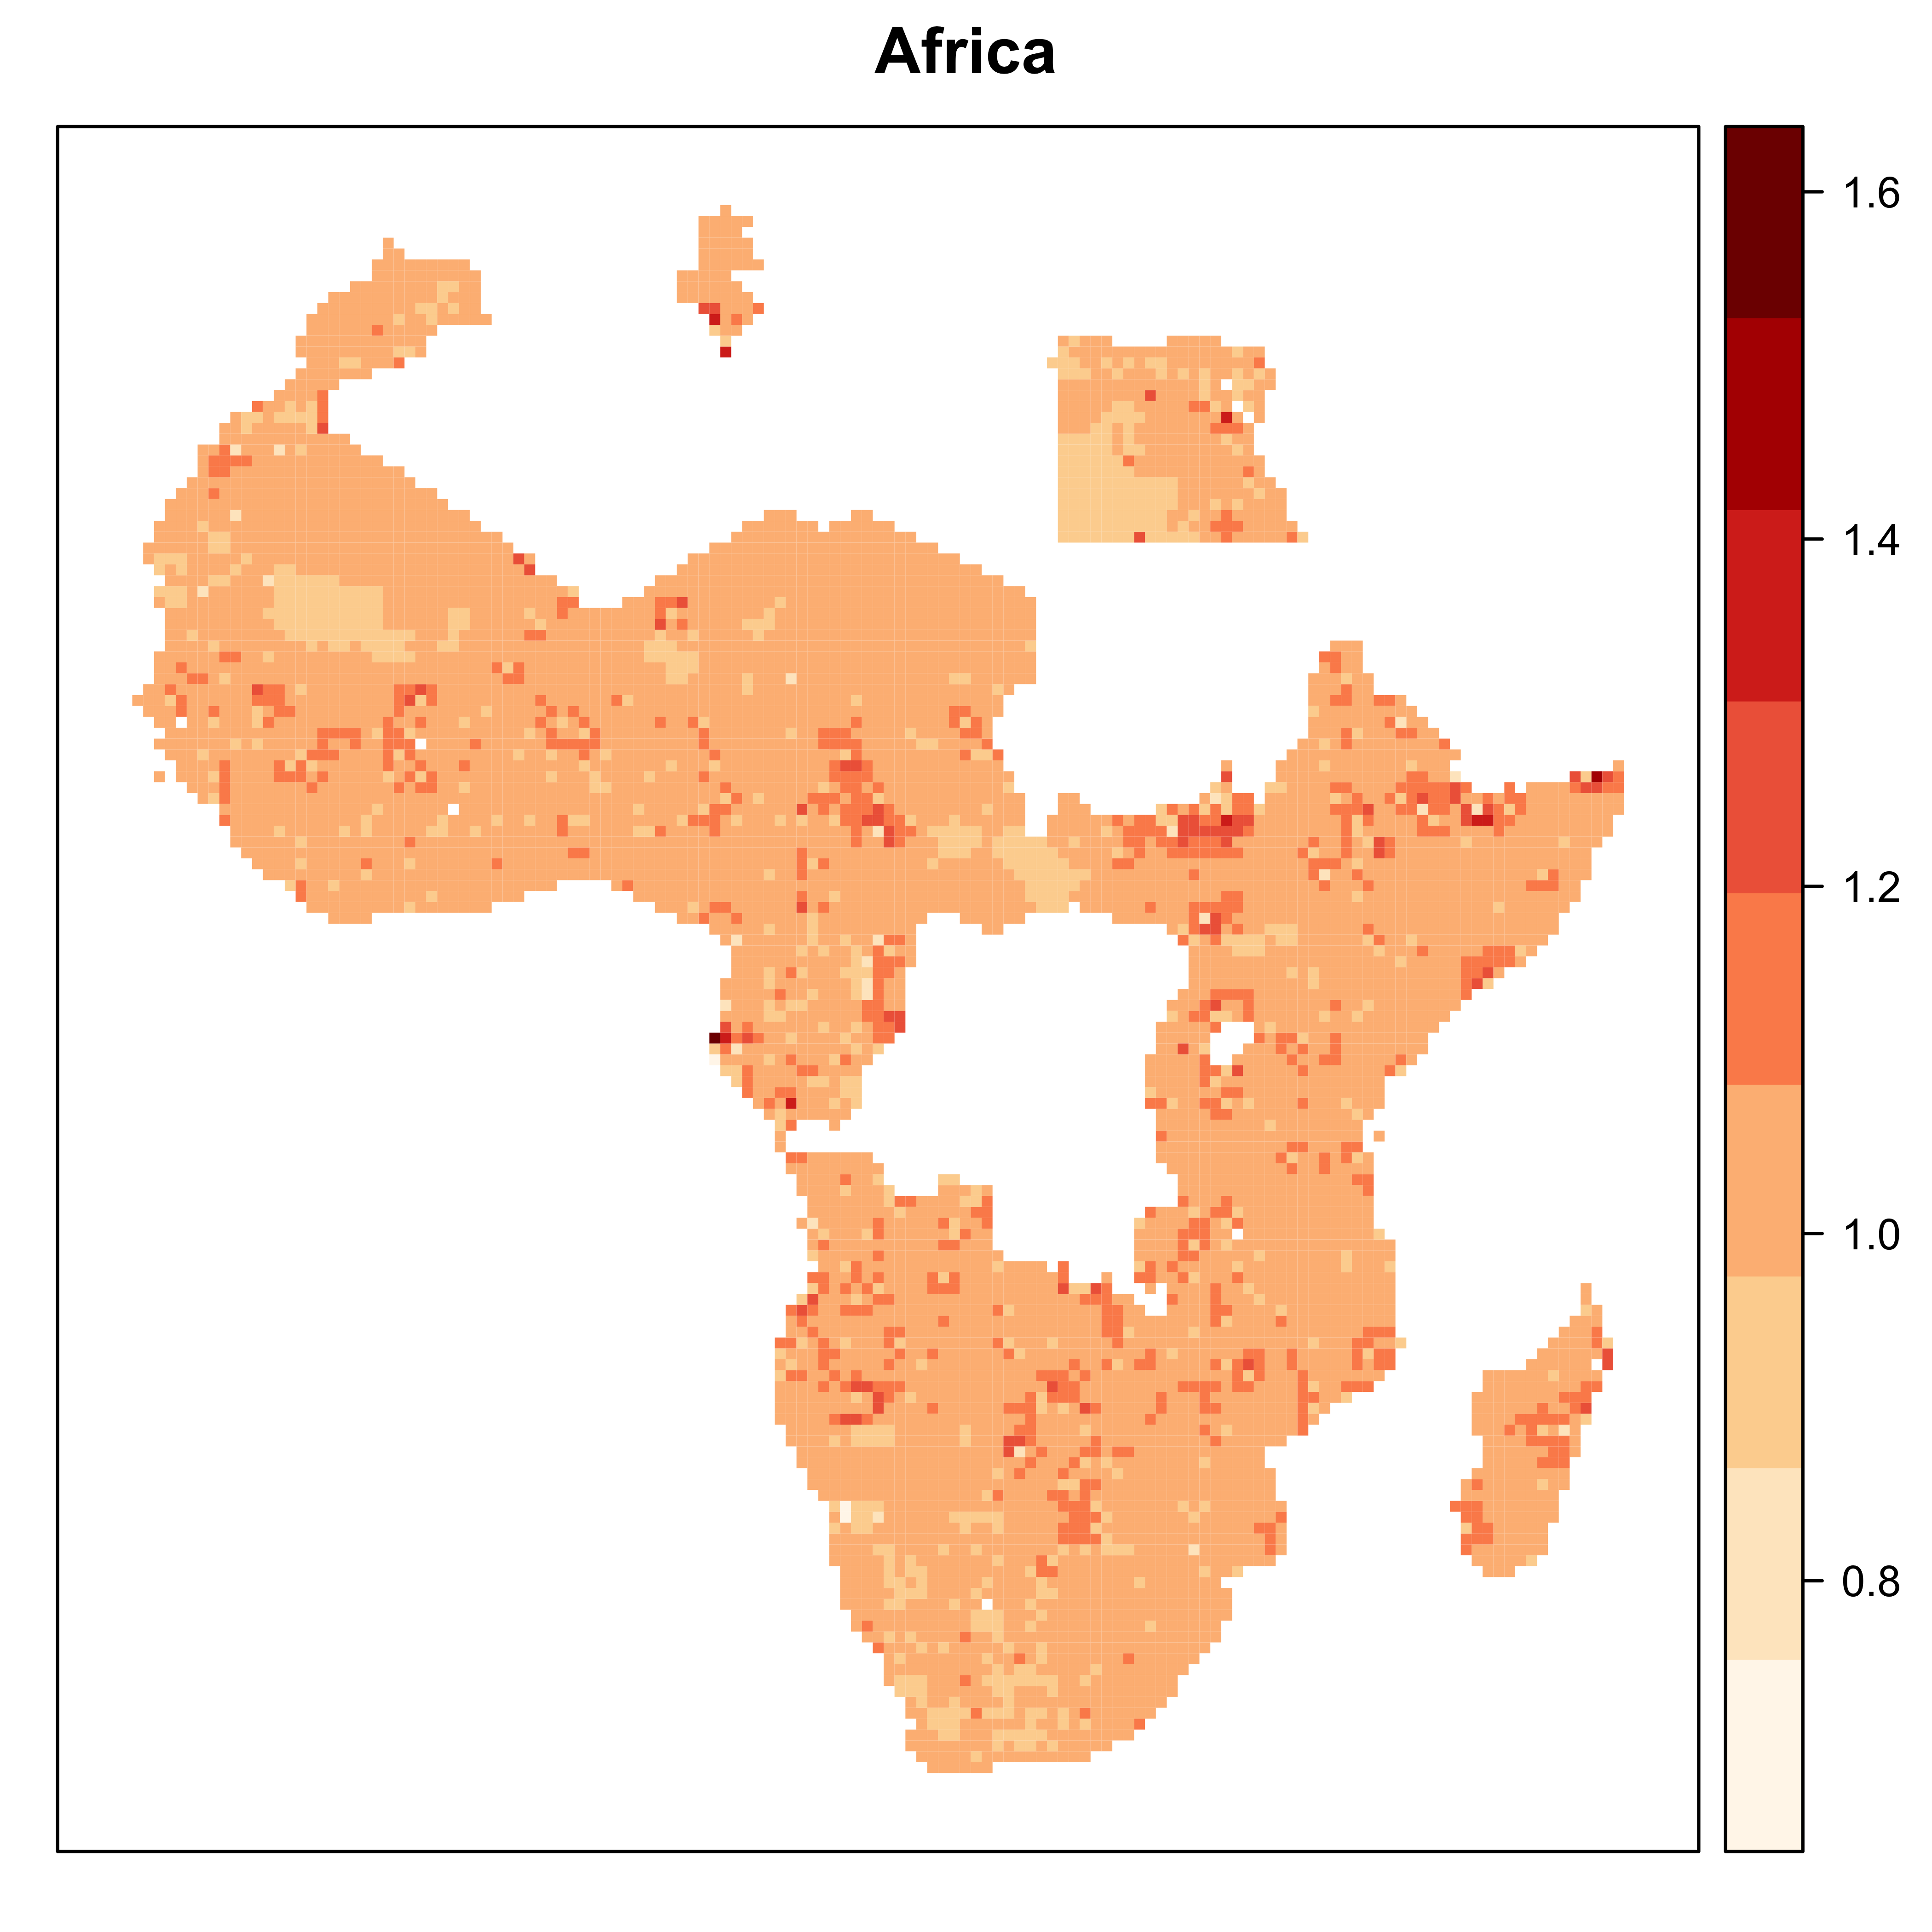
\includegraphics[width=0.65\textwidth,trim={1cm 4cm 1cm 5cm},clip]{../../Analysis/output/zeta_heatmaps/African_gridcells_zeta.png}

\label{fig:all_gridcells_by_zeta}
\mysubcaption{Africa as represented by 10,158 grid cells of 0.5 $\times$ 0.5 degrees. Cells coloured according to their Local Infrastructure Discrimination Index $\Lambda_{i}$. Darker cells would benefit from reallocating national infrastructure networks. Note that the hypothetical reallocation scenario is conducted on the country-level. Cells from different countries are hence not immediately comparable. Map's colouring follows an equal-interval rule such that every colour in the spectrum has an equal amount of members. This is to visualise the measure's variation but leads to unequal bracket-sizes for each colour.}
\end{figure}
% End Figure

Figure \ref{fig:all_gridcells_by_zeta}, lastly, displays the spatial variation of $\Lambda_{i}$ over all 10,000+ grid cells of the entire continent. When interpreting this map, note that grid cells are undergoing the reshuffling scenario solely within their respective country. National borders hence play a role and can at times even clearly be inferred from the printed map.\footnote{There are two reasons why I conduct the simulation procedure within countries and not over the entire African continent. One is computational; the requirements for numerically solving the model increase quadratically in the number of locations $\mathcal{I}$. The largest country in Africa (Algeria) is made up of almost 900 locations and already strains computing power quite heavily. Simulating all of Africa's 10,000+ locations at once is then almost unattainable with available technology. The second reason is interpretational; while lifting a country's roads from the ground and flexibly reshuffling them across the nation is already a fictitious scenario, it still operates within a government transport authority's locus of control. Regions disadvantaged by their own government can reasonably be considered discriminated against. This is less the case if one were to optimise over the entire continent. Without a central planning body for all of Africa, it is hard to interpret why a road in e.g. Tunisia should rather be moved into Namibia.}  Keeping this in mind, the map reveals substantial spatial variation in the index across the African continent. The luckiest region (in Namibia) stands to loose almost 30\% of total welfare if the fictitious social planner intervened and reshuffled roads away from it. On the other extreme of the spectrum, the residents of one grid cell in Gabon are missing out on a welfare hike of more than 50\%. On average, a grid cell gains 2.8 per cent of welfare, the median cell gains 1.7\%. Figure \ref{fig:APP:histogram_lambda} in the appendix plots the distribution of $\Lambda_{i}$, which roughly follows a normal distribution. In Figure \ref{fig:all_gridcells_by_zeta}, abandoned regions are clearly displaying spatial correlation with large neighbouring swaths of land collectively missing out on infrastructure improvements in certain countries. This begs the conclusion that countries do not just overlook single grid cells but rather live with vast stretches of disadvantaged regions. The index is evidently representing more than just haphazard noise. In the following sections, I analyse patterns behind this heterogeneity of infrastructure discrimination over space.
% End Chapter

\section{An Empirical Investigation into Africa's Trade Network Inefficiencies}
\label{chap:results}
% Chapter
Why are some African roads not in the right place to promote beneficial trade? To investigate which areas have too much or too little infrastructure, I employ the \emph{Local Infrastructure Discrimination Index} $\Lambda_{i}$ as dependent variable in a standard OLS regression setting. In the base specification, I estimate
\begin{equation}
  \Lambda_{i,c} = \beta v_{i,c} + \textbf{X}_{i,c}\gamma + \delta_{c} + \epsilon_{i,c}
  \label{eq:grid_ols}
\end{equation}
for a variety of different independent variables $v_{i,c}$ of grid cell $i$ in country $c$. $\delta_{c}$ denotes country fixed effects, $\textbf{X}_{i,c}'$ is a vector of controls, and $\beta$ is the coefficient of interest. The dependent variable $\Lambda_{i,c}$ roughly follows a normal distribution and I hence do not transform it. As apparent in Figure \ref{fig:all_gridcells_by_zeta}, local infrastructure discrimination displays autocorrelation over space causing the error term $\epsilon_{i,c}$ to not be distributed independently. To account for this problem, I follow \cite{Bester_Inferencedependentdata_2011} and construct a higher-level spatial grid of 3 degrees latitude by 3 degrees longitude and cluster standard errors within each of these higher-level grid cells. Errors are  allowed to covary within each cluster, but not between them. This technique draws its power from constructing clusters in the most arbitrary manner possible without relying on potentially endogenous partitions like national borders or administrative units \citep[see e.g.][]{Michaels_ResettingUrbanNetwork_2017}.\footnote{There are 332 such clusters. Since 3 degrees is evenly divisible by the observation-level grid cell size of 0.5 degrees, each cluster in principle fits 36 observations. The median cluster does indeed comprise 36 cells, but some border-regions fit fewer observations. On average, there are 31 observations in a cluster.}

Including country fixed effects is of particular importance, as $\Lambda_{i}$ is constructed by optimising trade flows within each country separately. Larger, wealthier, or more urbanised countries have more flexibility in reallocating their transport network. A grid cell in Egypt is hence not directly comparable to one in Sierra Leone.  Country fixed effects account for this underlying heterogeneity and make observations comparable internationally. The vector of controls $\textbf{X}_{i,c}'$ captures observable characteristics of each grid cell that plausibly account for some of the variation in $\Lambda_{i}$. \cite{Henderson_GlobalSpatialDistribution_2018} show that a surprisingly parsimonious set of geographical and agricultural covariates explains a substantial part of the global variation in economic activity. Making use of their data, I include in $\textbf{X}$ each grid cell's average altitude, average temperature and precipitation, land suitability for agriculture, length of the annual growing period, and an index for the stability of malaria transmission. I also include mutually exclusive (and collectively exhaustive) dummy variables classifying each grid cell into one of twelve predominant vegetation regions \citep[or \emph{Biomes}, see][]{Henderson_GlobalSpatialDistribution_2018}.\footnote{Only eight of the twelve vegetation patterns are actually present on the African continent, the other indicators (biomes 4, 6, 8, and 11) are dropped from consideration.} To flexibly control for any broad geographic trend over the entire continent, I additionally add fourth-order polynomials of both latitude and longitude for each grid cell. To take into account that some regions have a natural advantage in conducting trade, I also include indicators for whether a grid cell's centroid is within 25 kilometres of a natural harbour, big lake, or navigable river respectively \citep[again using data from][]{Henderson_GlobalSpatialDistribution_2018}. Lastly, to account for potential gravitational trade forces from abroad, I create and include a dummy for whether a cell is at the border of a country's network and hence has less than eight immediate neighbours.

I call the set of controls outlined so far \emph{``Geographic Controls''}. They are in principle unaffected by human decisions about the design of trade networks and therefore plausibly exogeneous. Another set of covariates, however, poses more difficulties. These are the variables that were already used to calibrate the optimal reallocation simulation from above, namely a cell's population, light output, ruggedness, and classification into urban and rural.\footnote{Recall that population and output were components of the planner's problem, ruggedness went into the cost of building new infrastructure $\delta^{I}_{i,k}$, and the urban/rural classification determined which good a cell produced.} I call these \emph{``Simulation Controls''}. It is crucial to be aware that $\Lambda_{i}$ is, among others, already a product of the intricate interplay between these factors. There is hence a danger for plain OLS to detect a spurious, mechanical relationship between them, potentially biasing results. On the other hand, not controlling for the spatial distribution of people and economic activity creates the risk of confounding estimates by means of omitted variable bias. To confront this dilemma, I always report estimates with and without the set of simulation controls. As I will demonstrate, results turn out to be largely similar between the two, hinting at the highly non-linear genesis of $\Lambda_{i}$.\footnote{Since they are partially determined by variables from the set of geographic controls, population and night lights can also be seen as \emph{``bad controls''} in the sense of \cite{Angrist_MostlyHarmlessEconometrics_2008}. They warn against controlling for any covariate that could also be interpreted as an outcome of some of the other regressors. Again, I counter this potential fallacy by always reporting estimates with and without the set of simulation controls.} Table \ref{tab:APP:basic_corrs} in the appendix prints basic correlations of my various control sets with the outcome $\Lambda_{i}$. On average, my model reallocates roads towards border cells, as well as colder and more malaria-prone areas, and takes infrastructure away from more illuminated grid cells. Ruggedness, population, the classification of urban and rural, or fourth-order geographic trends do not systematically predict variations in $\Lambda_{i}$.

My measure of network inefficiency only pertains to systems of goods trade. As discussed above, there are clearly other rational motivations for building roads, mainly facilitating the commute of people to large administrative hubs -- most immediately, a nation's capital. To ensure that my results are not driven by systematic ignorance of these not-for-trade roads, I re-estimate every model while excluding grid cells containing a country's capital. Unless otherwise reported, this leaves results virtually unchanged.

In this paper, I investigate three potential sources of network inefficiency in Africa: colonial era infrastructure investments, ethnic power relations, and foreign aid. Each individual setting faces different challenges to identification but they are all based on the framework outlined above. The following sections present empirical strategies and results for all three strands of inquiry.

\subsection{Colonial Infrastructure Investments}
At the Berlin Conference of 1884--1885, European powers unilaterally decided to split up the African continent into spheres of influence amongst themselves, setting off what is known as the \emph{Scramble for Africa}. The colonising powers rushed to secure areas of control, formed local administrative hierarchies, and set up extractive economies depriving the continent of its natural resources. The following decades went on to transform the continent in a multitude of dimensions. A large literature has investigated the long-run effects of colonial policies on contemporary comparative development in Africa, including institutional reforms \citep{Acemoglu_ColonialOriginsComparative_2001,Acemoglu_ReversalFortuneGeography_2002}, border design \citep{Michalopoulos_LongRunEffectsScramble_2016}, and human capital formation \citep{Wantchekon_EducationHumanCapital_2015}.

The colonial powers also transformed the landscape of many African regions by devising large scale infrastructure projects. Starting in the late 19th century, numerous railway lines were built to facilitate the transport of goods and troops through the vast newly appropriated territories. Between 1890 and 1960, British, French, Belgian, German, Italian, and Portuguese administrations all undertook efforts to permeate their colonies with more or less sophisticated railway networks \citep{Jedwab_PermanentEffectsTransportation_2016a}. There were two main motivations for this: supporting the extractive economies and ensuring military domination \citep{Jedwab_HistoryPathDependence_2017a}. On the one hand, rail tracks were used to transport crops and minerals from the fields and mines of the African heartland to the nearest harbour city from which they were shipped back to Europe. On the other hand, geopolitical considerations led the colonial governments to rapidly expand their network to showcase their military might and secure their spheres of influence.

In Nigeria, for example, the British colonial administration in the 1890s saw itself under increasing pressure to counter advances by the French into the northern parts of the country. In response, three major railway lines were built over the next two decades to connect the north with the southern coast \citep{Falola_historyNigeria_2008}. However, these were used not only for military purposes, but also to transport ground nuts, palm oil, and cocoa to the harbours in Lagos, Port Harcourt, and Calabar \citep{Ekundare_EconomicHistoryNigeria_1973}. Transporting goods between the various regions of the country had been relying on head porterage for centuries, rendering interregional trade in commodities all but impossible.\footnote{Until the construction of colonial railways, the only systematic interregional trade in many African countries had been the slave trade. Over five centuries leading up to the Berlin Conference about 18 million Africans were enslaved and traded out of the country, the majority by ship to the New World \citep{Nunn_LongtermEffectsAfrica_2008}.} Trips on the newly constructed lines were slow and arduous compared to modern standards, but nevertheless marked the first time goods and people could relatively easily travel between the different parts of the country \citep{Chaves_ReinventingWheelEconomic_2014}. As a result, Britain secured their strategic grip on Nigeria's north, extracted minerals and crops on a large scale, and saw export volumes skyrocket \citep{Falola_historyNigeria_2008,Woltjer_EconomicRationaleWest_2018}. Though they hardly ever directly benefited the local population, the construction of railroads could be seen as a transformative event for the Nigerian economy at the dawn of the 20$^{\textrm{th}}$ century.\footnote{Other case studies for Ghana \citep{Jedwab_PermanentEffectsTransportation_2016a}, Kenya \citep{Jedwab_HistoryPathDependence_2017a}, India \citep{Donaldson_RailroadsRajEstimating_2018}, or the US \citep{donaldson_railroads_2016,Swisher_ReassessingRailroadsGrowth_2017} describe similarly transformative impacts of railroad construction on the local economy at the time.}

Apart from boosting the development of trade and migration at the time, colonial railroads have also been found to have a persistent impact on the spatial organisation of economic activity today. \cite{Jedwab_PermanentEffectsTransportation_2016a} show how urbanisation started to centre around railway tracks in the decades following their construction. Even as most railway lines have fallen into disarray and road traffic has replaced trains as the most important means of transportation, economic activity today still clusters in places close to the former rail lines. \citeauthor{Jedwab_PermanentEffectsTransportation_2016a} see this as evidence that other spatial equilibria could have emerged, but placement of rail tracks facilitated the coordination on one of them.

Did the transport revolution coordinate the economy on an efficient spatial equilibrium? To investigate whether railways from the colonial period still have an impact on trade network inefficiency today, I overlay the 10,000+ grid cells of my data set with every railway line built by the colonial powers in Sub-Saharan Africa. Figure \ref{fig:Railroad_Map} prints in red 237 lines built between 1890 and the various independence dates. Data on railroad positioning comes from \cite{Jedwab_PermanentEffectsTransportation_2016a}, with the exception of South Africa, for which I manually digitise a map from \cite{Herranz-Loncan_publicbenefitRailways_2017}. No comparable data are available for Madagascar, Egypt, and the Maghreb countries, which also saw some colonial railway construction. As discussed below, findings are robust to excluding grid cells from these countries.

% Figure Maps of Rails
\begin{figure}
\centering
\caption{Colonial Railway Network}

\begin{subfigure}[c]{0.48\textwidth}
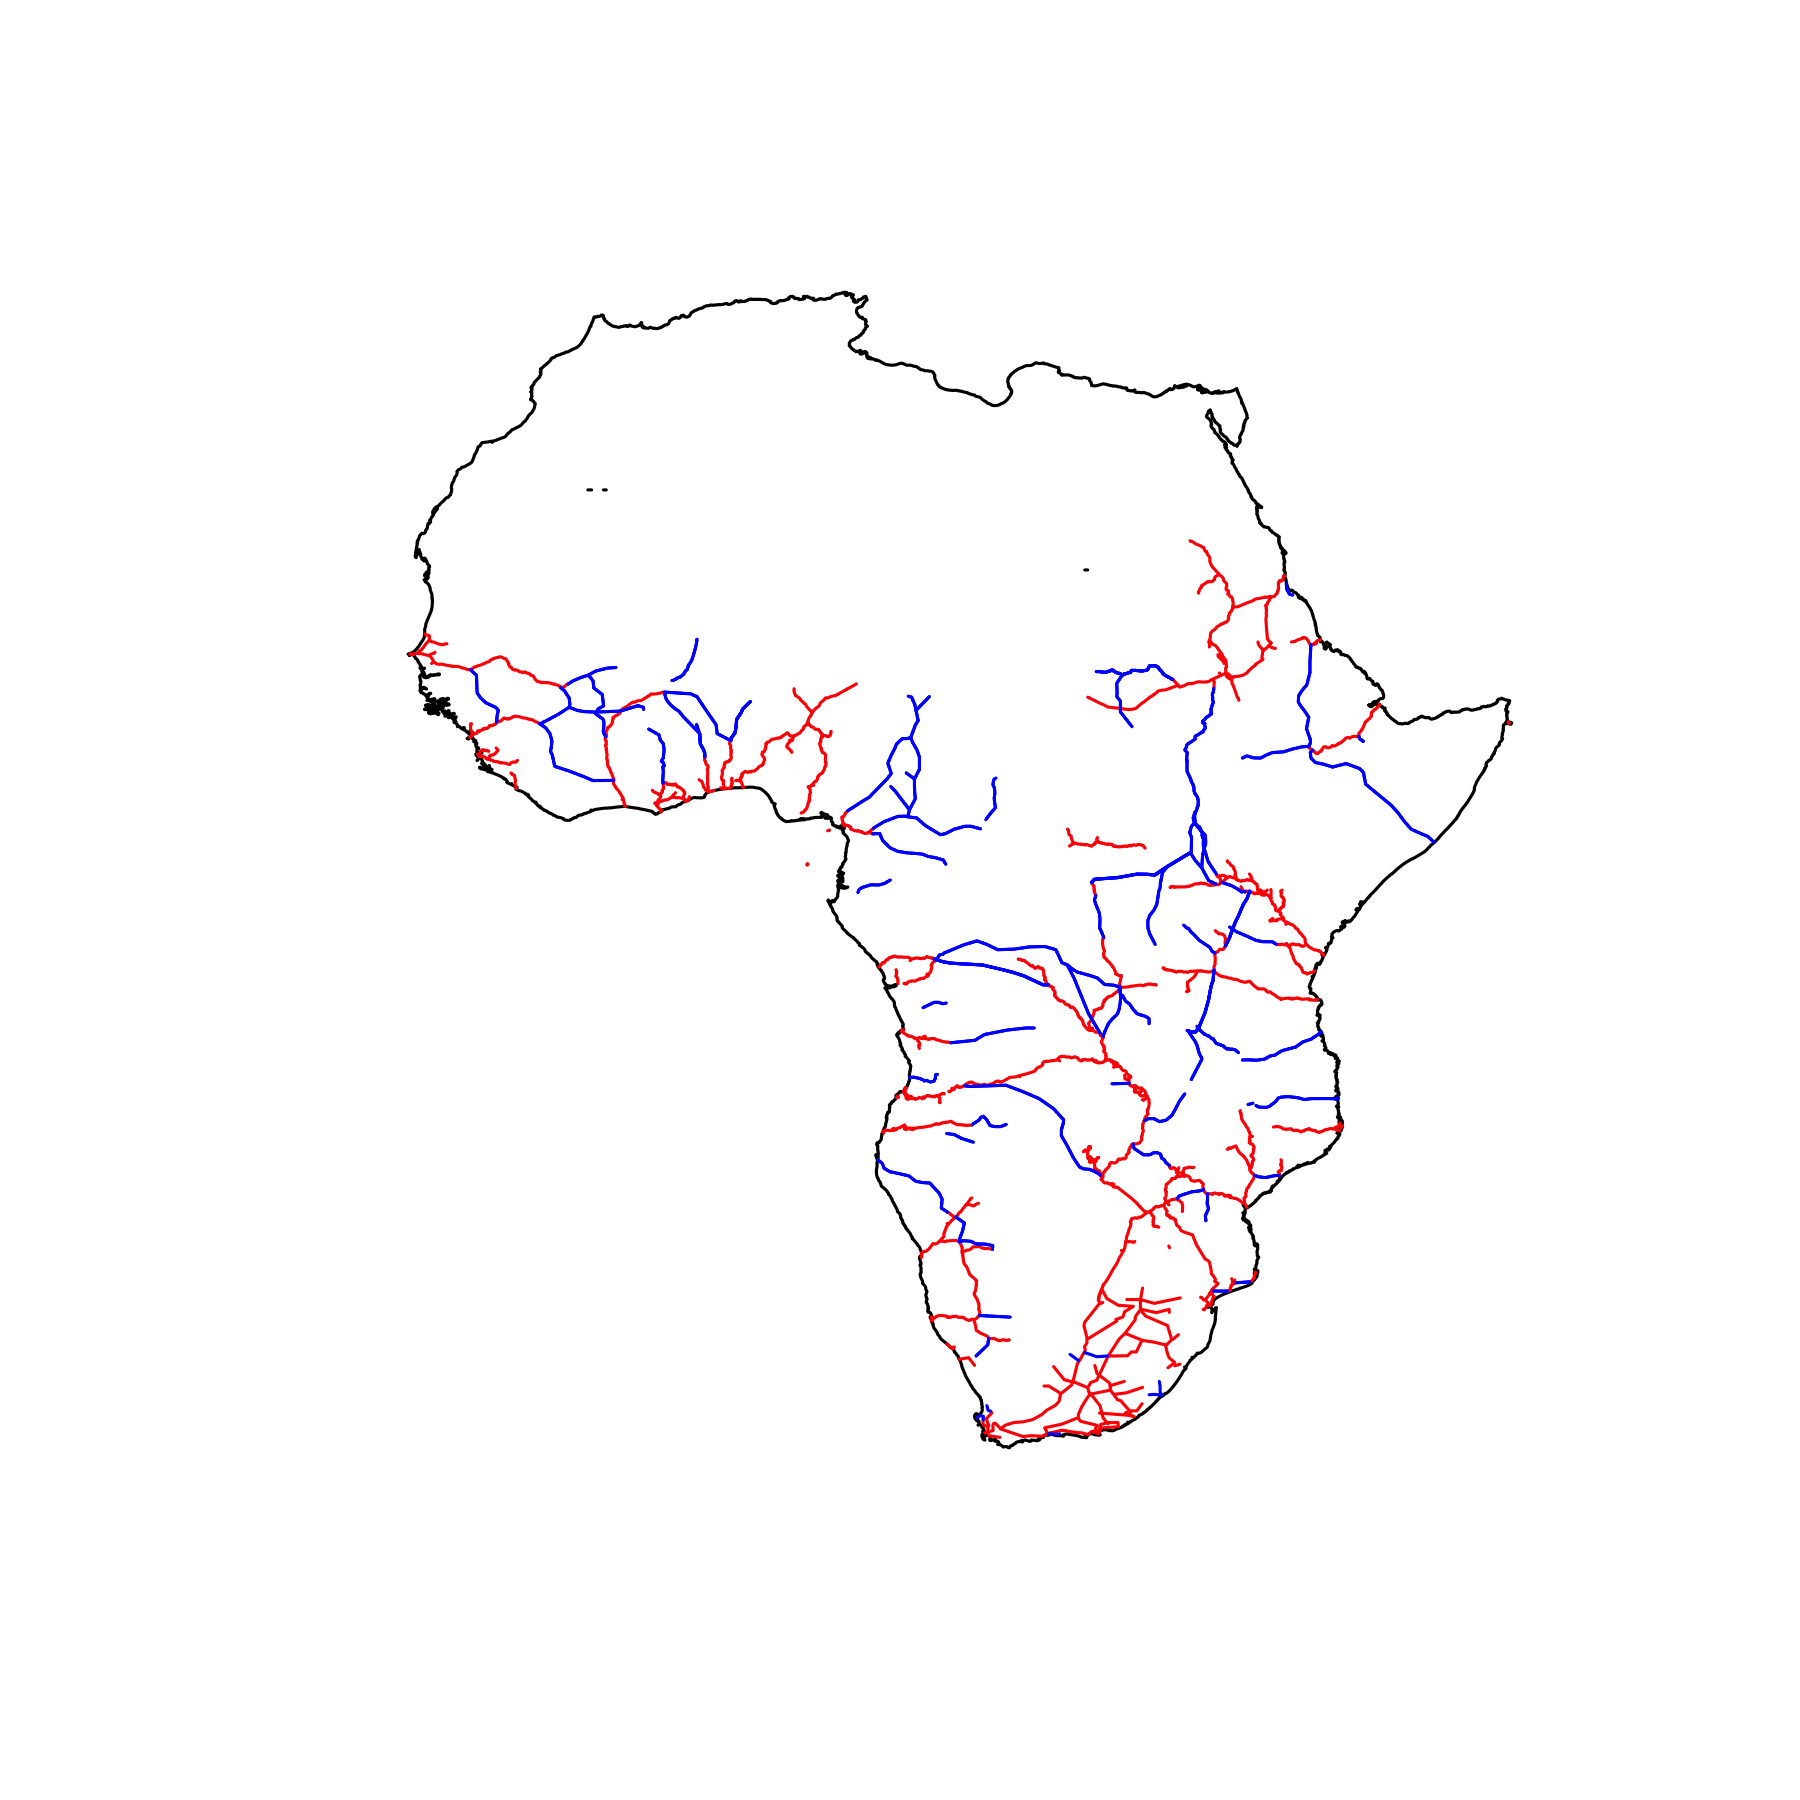
\includegraphics[width=\textwidth,trim={10cm 11cm 6cm 10cm},clip]{../../Analysis/output/other_maps/all_rails.png}
\caption{Colonial Rails (red) and Placebo Rails (blue)}
\label{fig:Railroad_Map}
\end{subfigure}
\begin{subfigure}[c]{0.48\textwidth}
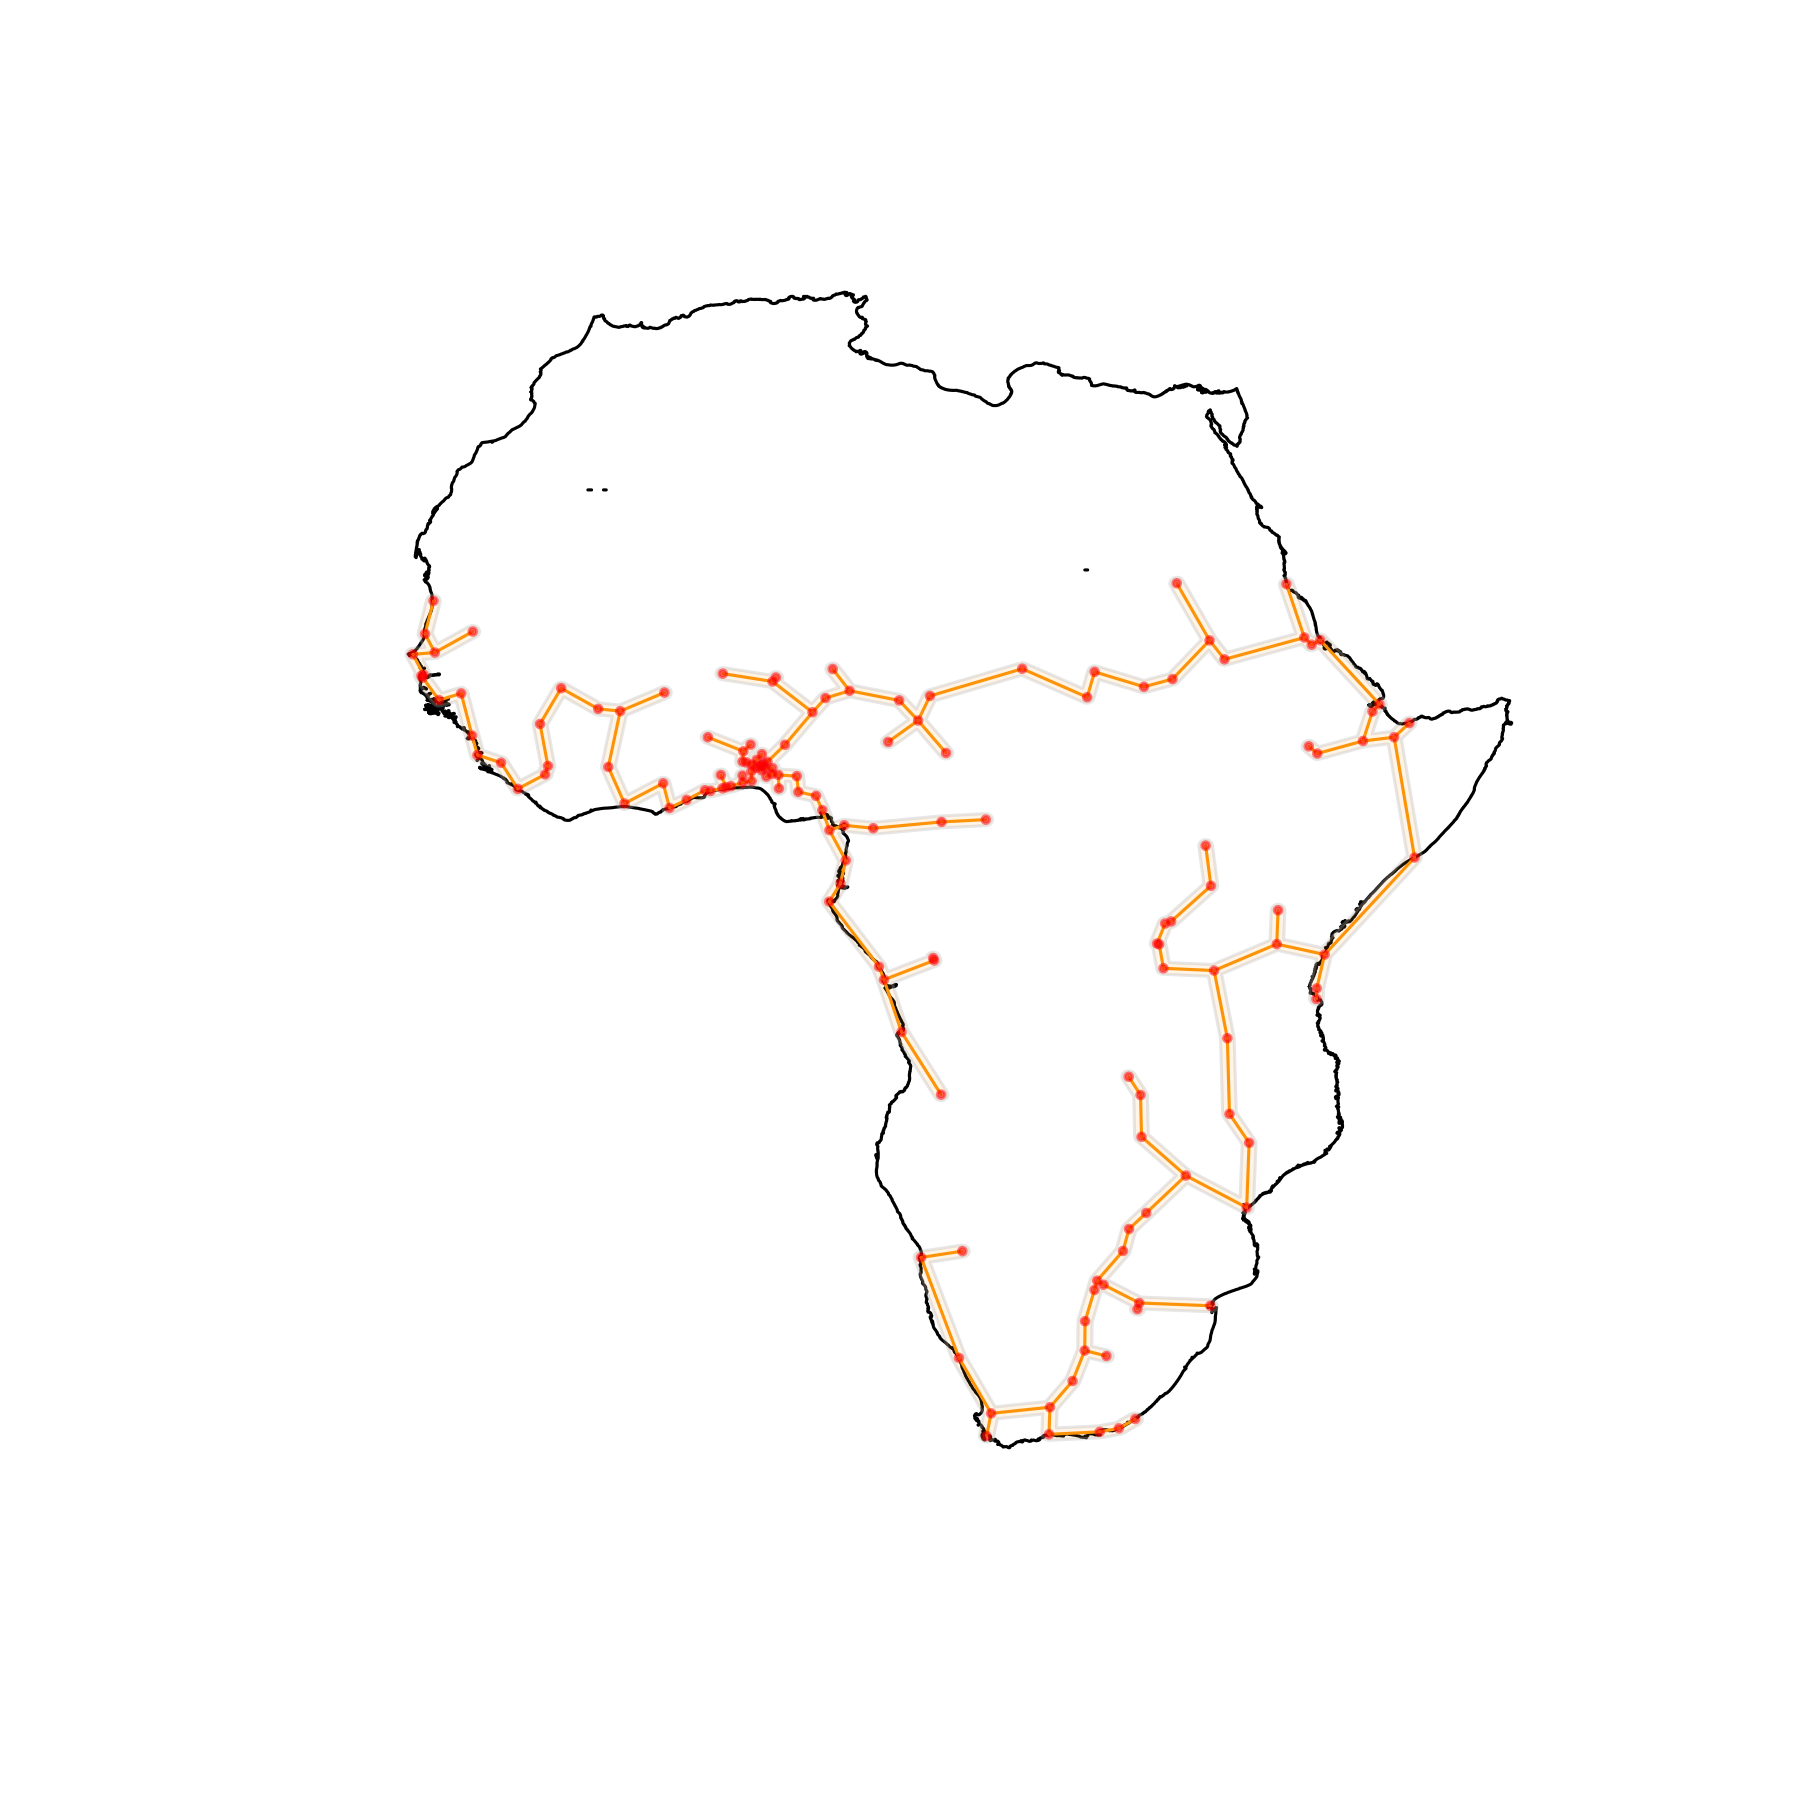
\includegraphics[width=\textwidth,trim={10cm 11cm 6cm 10cm},clip]{../../Analysis/output/other_maps/emst.png}
\caption{EMST Lines and Buffer}
\label{fig:EMST_Map}
\end{subfigure}

\label{fig:Rail Maps}
\mysubcaption{Maps displaying the network of railway lines and placebo railroads. Data from \cite{Jedwab_PermanentEffectsTransportation_2016a} and \cite{Herranz-Loncan_publicbenefitRailways_2017}. Subfigure (a) prints in red  railroads built by the colonial powers between 1890 and 1960. Lines that were initially planned but never actually built are printed in blue. Subfigure (b) prints the euclidean minimum spanning tree (EMST), connecting the initial urban network of 1900 (red dots) with the least amount of total rail kilometres \citep[see ][]{Jedwab_PermanentEffectsTransportation_2016a}. This is the rail system that would have minimised total infrastructure costs if the colonial powers had cooperated and jointly devised an ideal network. Subfigure (b) also prints a buffer of 40km around the EMST.}
\end{figure}
% End Figure

For every grid cell, I compute the total number of colonial railway kilometres crossing the cell. This serves as a tangible measure for the stock of physical transport capital invested into each region. The majority of cells (91\%) are not crossed by a colonial railway and hence have zero railroad kilometres. Those that are intersected by a line usually have between 20 and 60 railroad kilometres, while some important rail crossings or transport hubs have up to 100 kilometres of railroads (in a 55 by 55 kilometre cell nevertheless). This measure captures the intensive margin of colonial infrastructure investment. I also construct a measure of extensive margin railroad exposure by computing the distance from a cell's centroid to its closest rail line. Every railroad line comes with a classification of being constructed primarily for military purposes or mining purposes (or neither, or both), allowing for more nuanced further analysis. Lastly, to account for potential endogeneity concerns, I also compute the same statistics for a set of railway lines the colonisers planned, but never built. As \cite{Jedwab_PermanentEffectsTransportation_2016a} explain, these projects were not realised only for a series of arguably random historical events like unforeseeable cuts to financing, the outbreak of wars, or sudden retirements of administration officials. If any effects are to be attested to the construction of railroads during the colonial era, no impact should be found for such \emph{placebo} railroads. These tracks are printed in blue in Figure \ref{fig:Railroad_Map}.\footnote{Data for placebo lines also come from \cite{Jedwab_PermanentEffectsTransportation_2016a} and \cite{Herranz-Loncan_publicbenefitRailways_2017}.}

% Figure Table of RailKM_zeta
\begin{table}[t] \centering
  \caption{Colonial Railroads and Local Infrastructure Discrimination Index}
  \label{tab:RailKM_zeta}
  \resizebox{\textwidth}{!}{

  \begin{tabular}{@{\extracolsep{5pt}}lcccccccc}
  \\[-1.8ex]\hline
  \hline \\[-1.8ex]
   & \multicolumn{8}{c}{\textit{Dependent variable: Local Infrastructure Discrimination Index $\Lambda_{i}$}} \\
  \cline{2-9}
  \\[-1.8ex] & (1) & (2) & (3) & (4) & (5) & (6) & (7) & (8)\\
  \hline \\[-1.8ex]
   KM of Colonial Railroads & $-$0.0002$^{***}$ & $-$0.0001$^{***}$ & $-$0.0002$^{***}$ & $-$0.0002$^{***}$ &  &  &  &  \\
  & (0.0001) & (0.0001) & (0.0001) & (0.0001) &  &  &  &  \\
    & & & & & & & & \\
   KM of Colonial Placebo Railroads &  &  &  &  & 0.00004 & $-$0.0002 & $-$0.0002 & $-$0.0003 \\
  &  &  &  &  & (0.0003) & (0.0003) & (0.0003) & (0.0003) \\
    & & & & & & & & \\
  \hline \\[-1.8ex]
  Country FE &  & Yes & Yes & Yes &  & Yes & Yes & Yes \\
  Geographic controls &  &  & Yes & Yes &  &  & Yes & Yes \\
  Simulation controls &  &  &  & Yes &  &  &  & Yes \\
  Observations & 10,158 & 10,158 & 10,158 & 10,158 & 10,158 & 10,158 & 10,158 & 10,158 \\
  R$^{2}$ & 0.001 & 0.099 & 0.124 & 0.126 & 0.00000 & 0.098 & 0.122 & 0.124 \\
  \hline
  \hline \\[-1.8ex]
  \textit{Note:}  & \multicolumn{8}{r}{$^{*}$p$<$0.1; $^{**}$p$<$0.05; $^{***}$p$<$0.01} \\
  \end{tabular}

}

\mysubcaption{Results of estimation of equation \eqref{eq:grid_ols} on the sample of 0.5 $\times$ 0.5 degree grid cells for the entire African continent (excluding six small countries, see text). Dependent variable is the Local Infrastructure Discrimination Index $\Lambda_{i}$ for each grid cell. Columns (1)-(4) estimate the effect of colonial infrastructure investments as measured by the total number of colonial railroad kilometres crossing a cell. Starting with a simple univariate cross-section in (1), column (2) adds 49 country fixed effects. Column (3) adds geographic controls, consisting of altitude, temperature, average land suitability, malaria prevalence, yearly growing days, average precipitation, indicators for the 12 predominant agricultural biomes, indicators for whether a cell is within 25 KM of a natural harbour, navigable river, or lake, the fourth-order polynomial of latitude and longitude, and an indicator of whether the grid cell lies on the border of a country's network. Simulation controls are added in column (4) and are comprised of population, night lights, ruggedness, and a dummy for whether a cell is classified as urban. These indicators went into the original infrastructure reallocation simulation and are hence not orthogonal to $\Lambda$. Columns (5)--(8) repeat the estimations with railroads that were planned, but never built (``placebo railroads''). Results are robust to using only the subsample of 33 countries with colonial infrastructure investment as reported by \cite{Jedwab_PermanentEffectsTransportation_2016a}, plus South Africa (not reported). Results are also robust to excluding all grid cells containing a country's capital (not reported). Heteroskedasticity-robust standard errors are clustered on the 3 $\times$ 3 degree level and are shown in parentheses.}
\end{table}
% End Figure

Table \ref{tab:RailKM_zeta} displays results from OLS estimation of Equation \eqref{eq:grid_ols} with $\Lambda_{i}$ on the left hand side and total rail kilometres as explanatory variable $v_{i}$. Column (1) displays the plain cross-sectional relationship without controls and reveals a statistically significant negative association between the two variables. Grid cells with high colonial railroad investment have significantly lower infrastructure discrimination today. Recall that low values of $\Lambda_{i}$ correspond to regions losing welfare if the social planner were to optimally reallocate infrastructure. On a merely descriptive level, the negative estimate of column (1) hence implies that regions with colonial railroads crossing through them would on average see infrastructure (and welfare) redistributed to those areas without colonial investments. This plain correlational relationship is far from implying any form of causation. A score of other variables could instead be responsible for this observational association. To confront these reservations, columns (2) -- (4) gradually extend the set of observable controls. The point estimate and statistical significance of the persistence of railroads is robust to including country fixed effects, geographical controls, and simulation controls as described above. In the richest specification of column (4), every ten kilometres of colonial railway construction are associated with grid cells losing $0.2$ percentage points of welfare at the hand of areas without any investment.

The colonial authorities did not place railroads randomly. Decisions on where to invest in expensive transport infrastructure is rather subject to cost-benefit analyses, regional economic potential, and projections about which areas are expected to thrive. This poses a threat to identification as the construction of railroads does not constitute a perfect natural experiment. Rather, columns (1) -- (4) of Table \ref{tab:RailKM_zeta} estimate the joint effect of a region being selected as a site for railroad investment \emph{together} with the actual investment. If the selection process relies on unobservables characteristics that impact $\Lambda_{i}$ today, estimates will be biased.\footnote{One can make the case that, if anything, this bias might mask a much stronger effect in the same direction as in Table \ref{tab:RailKM_zeta}. If railroads were built in areas which were expected to do well in the future, these regions might be receiving more infrastructure from the social planner today. This would attenuate the negative effect in columns (1) -- (4). However, other potential directions for the bias are conceivable as well.} To isolate the effect of actual infrastructure investments, columns (5) -- (8) repeat the exercise for the set of placebo railroads. If these are assumed to have undergone the same planning process as actual railways, the regressions reveal the distorting power of site selection. None of the estimates are significantly different from zero, suggesting that the link in columns (1) -- (4) is a causal one. The construction of railways by the colonial powers cause affected regions to be too well off today. The results are virtually identical when using only the subsample of 34 countries for which data on colonial railroad placement are available, or excluding all grid cells containing a national capital (not reported).

The effects described in Table \ref{tab:RailKM_zeta} are small, yet remarkable. Across the African continent, areas that received large infrastructure investments a century ago are still \emph{too} well off given their position in the national trade network. In contrast, areas that were not crossed by tracks are inefficiently short on infrastructure today. To see that this is a non-trivial finding, note that, firstly, most of the colonial railway lines have been in disrepair for decades and thus do not immediately dictate trade flows today. Secondly, recall that the optimal network reallocation and construction of $\Lambda_{i}$ was based on roads and cars, not rails and trains. The implication is hence \emph{not} that colonial railway systems themselves are inadequate to efficiently sustain inter-regional trade today. Rather the transport revolution a century ago coordinated the entire economy into a certain spatial equilibrium, which persists even though it has become inefficient. African nations would benefit from moving to a better equilibrium, but are locked in the current state. The placement of colonial railroads set in motion a process of spatial sorting with people, output, and infrastructure clustering in locations which are suboptimal today. The social planner identifies this, seeks to overcome these misallocations, and move infrastructure away from regions once considered important by the colonisers. \citeauthor{Jedwab_PermanentEffectsTransportation_2016a} show that colonial investments helped the economy to coordinate on one of many spatial equilibria -- my findings suggest that this is not the optimal one.\footnote{Note that the spatial equilibrium induced by colonial railroads could have still been optimal \emph{at the time}. My argument solely concerns the persistent effects of investments a century ago on network efficiency \emph{today}.}

% Figure Table RailKM_mining_military
\begin{table}[t] \centering
  \caption{Heterogeneous Effects of Colonial Railroads}
  \label{tab:RailKM_mining_military}
  \resizebox{\textwidth}{!}{


  \begin{tabular}{@{\extracolsep{5pt}}lcccccccc}
  \\[-1.8ex]\hline
  \hline \\[-1.8ex]
   & \multicolumn{8}{c}{\textit{Dependent variable: Local Infrastructure Discrimination Index $\Lambda_{i}$}} \\
  \cline{2-9}
  \\[-1.8ex] & (1) & (2) & (3) & (4) & (5) & (6) & (7) & (8)\\
  \hline \\[-1.8ex]
   KM of Rails & $-$0.0002$^{***}$ & $-$0.0002$^{***}$ &  &  & $-$0.0002$^{**}$ & $-$0.0002$^{**}$ &  &  \\
   \hspace*{3mm} for Military Purposes & (0.0001) & (0.0001) &  &  & (0.0001) & (0.0001) &  &  \\
    & & & & & & & & \\
   KM of Rails  &  &  & $-$0.0001 & $-$0.0001 & $-$0.0001 & $-$0.0001 &  &  \\
  \hspace*{3mm} for Mining Purposes &  &  & (0.0001) & (0.0001) & (0.0001) & (0.0001) &  &  \\
    & & & & & & & & \\
    KM of Rails &  &  &  &  &  &  & $-$0.0003$^{***}$ &  \\
  \hspace*{3mm} within EMST Buffer &  &  &  &  &  &  & (0.0001) &  \\
     & & & & & & & & \\
    KM of Rails  &  &  &  &  &  &  &  & $-$0.0001$^{**}$ \\
  \hspace*{3mm} outside EMST Buffer &  &  &  &  &  &  &  & (0.0001) \\
     & & & & & & & & \\
  \hline \\[-1.8ex]
  Country FE & Yes & Yes & Yes & Yes & Yes & Yes & Yes & Yes \\
  Geographic controls & Yes & Yes & Yes & Yes & Yes & Yes & Yes & Yes \\
  Simulation controls &  & Yes &  & Yes &  & Yes & Yes & Yes \\
  Observations & 10,158 & 10,158 & 10,158 & 10,158 & 10,158 & 10,158 & 10,039 & 10,039 \\
  R$^{2}$ & 0.123 & 0.125 & 0.122 & 0.124 & 0.123 & 0.125 & 0.126 & 0.125 \\
  \hline
  \hline \\[-1.8ex]
  \textit{Note:}  & \multicolumn{8}{r}{$^{*}$p$<$0.1; $^{**}$p$<$0.05; $^{***}$p$<$0.01} \\
  \end{tabular}

}

\mysubcaption{Replication of estimations of Table \ref{tab:RailKM_zeta} in estimating effects of colonial railroads on the Local Infrastructure Discrimination Index $\Lambda$. Colonial rails are classified as built for military or mining purposes (or neither or both) by \cite{Jedwab_PermanentEffectsTransportation_2016a}. Columns (7)-(8) distinguish between railway kilometres within and outside the 40km-wide buffer around the euclidean minimum spanning tree (EMST) of the initial urban network. Sample in columns (7)-(8) excludes the 119 grid cells that comprise the nodes of the EMST, as proposed by \citeauthor{Jedwab_PermanentEffectsTransportation_2016a}. Geographic controls consist of altitude, temperature, average land suitability, malaria prevalence, yearly growing days, average precipitation, indicators for the 12 predominant agricultural biomes, indicators for whether a cell is within 25 KM of a natural harbour, navigable river, or lake, the fourth-order polynomial of latitude and longitude, and an indicator of whether the grid cell lies on the border of a country's network. Simulation controls are comprised of population, night lights, ruggedness, and a dummy for whether a cell is classified as urban. Results are robust to using only the subsample of 34 countries with colonial infrastructure investment, with only the estimate in column (8) estimated less precisely (but still $p<0.1$). Results are also robust to excluding all grid cells containing a country's capital (not reported). Heteroskedasticity-robust standard errors are clustered on the 3 $\times$ 3 degree level and are shown in parentheses.}
\end{table}
% End Figure

Which railways were responsible for coordinating African economies into a suboptimal spatial equilibrium? To further understand the forces behind this dynamic, I split the sample of colonial railways along their initial construction purpose. As discussed above, most tracks were built with military or mining considerations in mind. Similarly to the exercise above, I thus separately calculate the total number of mining and military railroad kilometres crossing a cell, respectively. Table \ref{tab:RailKM_mining_military} repeats the estimations from above for both subsets of railways. As can be inferred from columns (1) -- (6), the effect is exclusively driven by railways built for military purposes. The social planner seeks to take welfare away from regions which were crossed by lines built for strategic military domination. Railroads constructed to support the mining trade are not associated with areas too well off today. This distinction holds both when including the variables separately (columns 1 -- 4) or jointly (columns 5 -- 6).

This finding offers an intuitive understanding of how the current spatial distribution is inefficient. All colonial infrastructure investments spurred urbanisation close-by, regardless of their construction purpose. Since mining lines arguably cross areas that are still important trade routes today, the social planner sees no need to reorganise infrastructure away from them. Areas surrounding rails built with military motives in mind, however, have since lost their strategic importance. As the nature of military domination, state authority, and conflict have changed since the 19th century, there is no immediate value to clustering economic activity and infrastructure close to former military lines anymore. It is those sunk investments that skew the spatial equilibrium towards an inefficient equilibrium.

To further differentiate railroad lines by their strategic importance, I follow \cite{Jedwab_PermanentEffectsTransportation_2016a} and \cite{Faber_TradeIntegrationMarket_2014} and construct the euclidean minimum spanning tree (EMST) for the African urban network in 1900. This is the network that minimises total euclidean distance of edges while ensuring that all nodes are connected to each other. Following \citeauthor{Jedwab_PermanentEffectsTransportation_2016a}, I take as nodes all African cities with a population of over 10,000 people in 1900.\footnote{This amounts to 119 nodes. 105 of these are reported by \cite{Jedwab_PermanentEffectsTransportation_2016a}, 14 are in South Africa and from a map in \cite{Herranz-Loncan_publicbenefitRailways_2017}.} Figure \ref{fig:EMST_Map} prints the cities and the tree connecting them. I then construct a 40 kilometre buffer around the EMST lines and split all colonial railways by whether or not they are located within this buffer.\footnote{The choice of 40 kilometres is arbitrary and directly follows \cite{Jedwab_PermanentEffectsTransportation_2016a}.} Intuitively, rails within the buffer have more strategic military importance than those outside it. Railroads built to support regional trade do not necessarily have to be on the straight line between major cities -- lines with the aim of quickly transporting troops do.

Columns (7) -- (8) of Table \ref{tab:RailKM_mining_military} estimate the heterogeneous effects of both kinds of railway kilometres. Following \citeauthor{Jedwab_PermanentEffectsTransportation_2016a}, I drop grid cells containing one of the 119 nodes spanning the EMST. Results are inconclusive. While railroad kilometres inside the buffer around the EMST are strongly associated with areas being too well off today, the same holds to a lesser degree to those outside of it. The estimate for rails close to the EMST is three times as large as the one for rails far away, however both are significantly smaller than zero. This leads to the conclusion that all colonial railways clustered economic activity in inefficient locations, only those built for strategic purposes did so even more. The social planner would like to reorganise infrastructure away from all former railway areas, but she would start at those constructed for geopolitical reasons.

% Figure Table RailBlocks_zeta
\begin{table}[t] \centering
  \caption{General Equilibrium Effects of Colonial Railroads}
  \label{tab:RailBlocks_zeta}
  \resizebox{\textwidth}{!}{


  \begin{tabular}{@{\extracolsep{5pt}}lcccccccc}
  \\[-1.8ex]\hline
  \hline \\[-1.8ex]
   & \multicolumn{8}{c}{\textit{Dependent variable: Local Infrastructure Discrimination Index $\Lambda_{i}$}} \\
   \cline{2-9}
     \\[-1.8ex]
   & \multicolumn{6}{c}{\small Full Sample} & \multicolumn{2}{c}{\small Restricted Sample} \\
  \cline{2-7} \cline{8-9}
  \\[-1.8ex] & (1) & (2) & (3) & (4) & (5) & (6) & (7) & (8)\\
  \hline \\[-1.8ex]
   $<10$ KM to Colonial Railroad & $-$0.013$^{***}$ & $-$0.015$^{***}$ & $-$0.017$^{***}$ &  &  &  & $-$0.014$^{***}$ &  \\
    & (0.003) & (0.004) & (0.004) &  &  &  & (0.004) &  \\
    & & & & & & & & \\
   $10-20$ KM to Colonial Railroad & $-$0.013$^{***}$ & $-$0.016$^{***}$ & $-$0.017$^{***}$ &  &  &  & $-$0.015$^{***}$ &  \\
  & (0.003) & (0.004) & (0.004) &  &  &  & (0.004) &  \\
    & & & & & & & & \\
   $20-30$ KM to Colonial Railroad & $-$0.002 & $-$0.004 & $-$0.005 &  &  &  & $-$0.005 &  \\
  & (0.004) & (0.004) & (0.004) &  &  &  & (0.004) &  \\
    & & & & & & & & \\
   $30-40$ KM to Colonial Railroad & 0.010$^{**}$ & 0.008$^{*}$ & 0.007 &  &  &  & 0.007 &  \\
  & (0.005) & (0.005) & (0.005) &  &  &  & (0.005) &  \\
    & & & & & & & & \\
   $<10$ KM to Colonial Placebo Railroad &  &  &  & $-$0.005 & $-$0.006 & $-$0.006 &  & $-$0.007$^{*}$ \\
  &  &  &  & (0.004) & (0.004) & (0.004) &  & (0.004) \\
    & & & & & & & & \\
   $10-20$ KM to Colonial Placebo Railroad &  &  &  & $-$0.003 & $-$0.004 & $-$0.005 &  & $-$0.005 \\
  &  &  &  & (0.005) & (0.005) & (0.005) &  & (0.005) \\
    & & & & & & & & \\
   $20-30$ KM to Colonial Placebo Railroad &  &  &  & $-$0.001 & $-$0.001 & $-$0.001 &  & $-$0.004 \\
  &  &  &  & (0.004) & (0.004) & (0.004) &  & (0.004) \\
    & & & & & & & & \\
   $30-40$ KM to Colonial Placebo Railroad &  &  &  & 0.007 & 0.006 & 0.005 &  & 0.003 \\
  &  &  &  & (0.004) & (0.004) & (0.004) &  & (0.004) \\
    & & & & & & & & \\
  \hline \\[-1.8ex]
  Country FE & Yes & Yes & Yes & Yes & Yes & Yes & Yes & Yes \\
  Geographic controls &  & Yes & Yes &  & Yes & Yes & Yes & Yes \\
  Simulation controls &  &  & Yes &  &  & Yes & Yes & Yes \\
  Observations & 10,158 & 10,158 & 10,158 & 10,158 & 10,158 & 10,158 & 6,362 & 6,362 \\
  R$^{2}$ & 0.101 & 0.126 & 0.129 & 0.099 & 0.123 & 0.125 & 0.121 & 0.115 \\
  \hline
  \hline \\[-1.8ex]
  \textit{Note:}  & \multicolumn{8}{r}{$^{*}$p$<$0.1; $^{**}$p$<$0.05; $^{***}$p$<$0.01} \\
  \end{tabular}

}

\mysubcaption{Effects of various distance-intervals on the Local Infrastructure Discrimination Index $\Lambda$. Explanatory covariates are dummy-variables indicating whether a cell's centroid is within X kilometres to its closest colonial railroad. Distance larger than 40 kilometres is the omitted category. Geographic controls consist of altitude, temperature, average land suitability, malaria prevalence, yearly growing days, average precipitation, indicators for the 12 predominant agricultural biomes, indicators for whether a cell is within 25 KM of a natural harbour, navigable river, or lake, the fourth-order polynomial of latitude and longitude, and an indicator of whether the grid cell lies on the border of a country's network. Simulation controls are comprised of population, night lights, ruggedness, and a dummy for whether a cell is classified as urban. Columns (1)-(3) examine the effect of actually built colonial railroads. Columns (4)-(6) repeat these calculations with railroads that were planned, but never built (``placebo railroads''). Columns (7)-(8) restrict the sample to the 32 countries on which data for colonial railways are available. Results are robust to excluding all grid cells containing a country's capital (not reported). Heteroskedasticity-robust standard errors are clustered on the 3 $\times$ 3 degree level and are shown in parentheses.}
\end{table}
% End Figure

So far, my empirical analysis has revolved around intensive margin effects of colonial railroads. Areas with more railways are stripped off more infrastructure by the social planner. But what about the extensive margin? Until how far away does the confounding effect of former train lines reach? Table \ref{tab:RailBlocks_zeta} displays results from regressing $\Lambda_{i}$ on a series of indicators denoting whether a grid cell's centroid is within certain distance intervals from its closest colonial rail line. Columns (1) -- (3) jointly estimate the effects of being within [0 -- 10], (10 -- 20], (20 -- 30], (30 -- 40], or (40+) kilometres from the closest passing railroad (with $(40+)$ being the omitted category). \cite{Jedwab_PermanentEffectsTransportation_2016a} find these intervals to be most significant in uncovering local reallocation effects. Apart from revealing the geographical extend to which colonial investments persist to skew spatial infrastructure systems today, these analyses can also help uncover general equilibrium effects. Are areas close to railroads better off at the expense of their immediate neighbours? Estimates from columns (1) -- (3) lend support to this claim. Grid cells with centroids less than 10 kilometres away from a passing railroad line are between $1.3$ and $1.7$ percentage points too well off compared to the omitted category. The estimate is significantly different from zero and robust to gradually introducing additional controls. The same dynamic also holds for cells within 20 kilometres of a passing line, and becomes undetectable further out. Moreover, one can even detect an adverse effect for cells between 30 and 40 kilometres away. Those cells would be granted additional welfare from redistributive efforts by the social planner. Though the estimate becomes increasingly imprecise and even insignificantly different from zero as further controls are introduced, the point estimate does not move by much. This is suggestive evidence that the confounding effect of colonial infrastructure policies is a locally contained. Areas blessed with a close-by railway line are still too well off today, which comes at the expense of their neighbouring regions just a few kilometres away.

To gain more confidence in the causal nature of this dynamic, columns (4) -- (6) again repeat the same exercise with placebo railroads. Of the twelve estimates produced, none is significantly different from zero. Columns (7) and (8) print results from estimating the same equation with the full set of controls, but restricting the sample to only grid cells in the 34 countries with data on colonial railway investment. In previous estimations, this restriction had virtually no effect on estimates' size, sign, and significance and hence was not explicitly reported. In the current case, however, truncating the sample by roughly a third produces a barely significant estimate for areas close to placebo railroads. All other results remain more or less the same. While this is certainly noteworthy, I believe this association to be merely spurious. In fact, by the law of large numbers, one would even statistically expect at least one of 16 placebo estimations to be within a p-value of less than $0.1$. The causal nature of local reallocation dynamics initiated by colonial infrastructure investments is hardly attenuated through this adverse finding.

In this section, I have shown how large scale transport infrastructure projects from the colonial era persist to skew the spatial composition of African trade networks towards a suboptimal state. Areas crossed by more colonial railway kilometres are too well off given their position in national trade systems today, even though these railroads were constructed over a century ago. Transport lines devised to meet military or strategic needs are associated with particularly strong effects. I also show that these projects set off local reallocation dynamics through which areas close to a line benefit at the expense of their neighbours. My results contribute to the plethora of studies examining the persistent impact of detrimental colonial policies on current development in Africa. However, recent history is hardly the only cause for heterogeneous development on the continent. In the following sections, I investigate two very different channels through which Africa's trade network might potentially be confounded: ethnic relations and foreign aid.

\subsection{Ethnic Relations}
An ominous legacy of the colonial era is the design of Africa's national borders. Drawn without much regard for local circumstances and with European rather than African interests in mind, many territories amalgamated various previously unrelated tribes and ethnicities under the umbrella of one nationality. After independence, most borders persisted and today African nations are among the most ethnically diverse in the world \citep{Alesina_Ethnicinequality_2016}.

A well established literature has investigated the impacts of ethnic diversity and identity on international comparative development \citep{Easterly_AfricaGrowthTragedy_1997,Alesina_EthnicDiversityEconomic_2005,gennaioli_modern_2007,Alesina_Ethnicinequality_2016}. More recently, a series of new studies has begun to shine light on the causes and effects of ethnicity-level heterogeneity within African countries. Ethnic homelands and tribes have been shown to be better developed when they are represented in national leadership \citep{Franck_DoesLeaderEthnicity_2012}, have more centralised deep rooted institutional systems \citep{Michalopoulos_PreColonialEthnicInstitutions_2013}, or simply are not split in two by artificial national border designs \citep{Michalopoulos_LongRunEffectsScramble_2016}.

The political economy of public good provision along ethnic lines presents an interesting case for the spatial imbalances in my dataset. Are ethnic homelands with less political clout systematically discriminated against in the provision of trade infrastructure? Is the substantial variation in infrastructure discrimination caused by government authorities channeling more transport investments towards members of their own ethnic group, even though other areas are more in need of better roads? Are African trade networks inefficient because of ethnic favouritism? If this were the case, the ethnicity-blind social planner would intervene and shuffle infrastructure away from favoured groups to achieve overall efficiency.

To analyse spatial patterns in the Local Infrastructure Discrimination Index $\Lambda$ over ethnic homelands, I follow \cite{Michalopoulos_PreColonialEthnicInstitutions_2013,Michalopoulos_NationalInstitutionsSubnational_2014,Michalopoulos_LongRunEffectsScramble_2016} and intersect an ethnolinguistic map of pre-colonial homelands from \cite{Murdock_Africaitspeoples_1959} with current national borders. Ethnicities present in more than one country count as multiple observations.\footnote{Ethnicity data are available for every country but Western Sahara.} Of the 835 inhabited homelands identified by \citeauthor{Murdock_Africaitspeoples_1959}, 314 are split in two or more parts by the current national borders, creating 1,212 ethnicity-country observations. I spatially aggregate my grid cell measure of network inefficiency $\Lambda_{i}$ onto the ethnicity-country level by assigning each grid cell an ethnicity based on its centroid location and weighing grid cells by their respective population.\footnote{Recall that on the grid cell level $\Lambda_{i}$ was defined as \begin{equation*}
  \Lambda_{i} = \frac{\textrm{Welfare under the optimal Infrastructure}_{i}}{\textrm{Welfare under the current Infrastructure}_{i}} = \frac{L_{i}u_{i}^{\textrm{optimal Infrastructure}}}{L_{i}u_{i}^{\textrm{current Infrastructure}}}
\end{equation*} To aggregate this onto the ethnic homeland level, I sum over all grid cells $i$ in homeland $h$ \begin{equation*}
  \Lambda_{h} = \frac{\sum_{i \in h}^{} L_{i}u_{i}^{\textrm{optimal Infrastructure}}}{\sum_{i \in h}^{}L_{i}u_{i}^{\textrm{current Infrastructure}}}
\end{equation*}} 280 ethnic homelands are too small to overlay with any grid cell centroid, leaving me with 932 observations. Figure \ref{fig:ethn_maps} presents the spatial variation of the Local Infrastructure Discrimination Index $\Lambda_{h}$ on the ethnicity-country level. The homeland which would benefit most from national reshuffling of roads is the tiny Tunisian part of the Ghadames homeland. This area was identified as an oil basin in the 1990s, stands to gain more than 40\% of welfare from reallocating national roads, and hence arguably presents an outlier \citep{Echikh_Geologyhydrocarbonoccurrences_1998}. Other ethnicities that are discriminated against mostly by the current network are the Kababish in Sudan (25\%), the Bata in Cameroon (24\%), or the Aushi in Congo-Kinshasa (23\%). The most disproportionally advantaged ethnic homelands in Africa are those of the Mober in Nigeria (who stand to lose 8\% of welfare if optimal networks were imposed) and the Sanga (7\%) and Kreish (11\%) of the Central African Republic.

% Figure Ethnicity Map
\begin{figure}
\centering
\caption{$\Lambda_{h}$ over Ethnic Homelands}

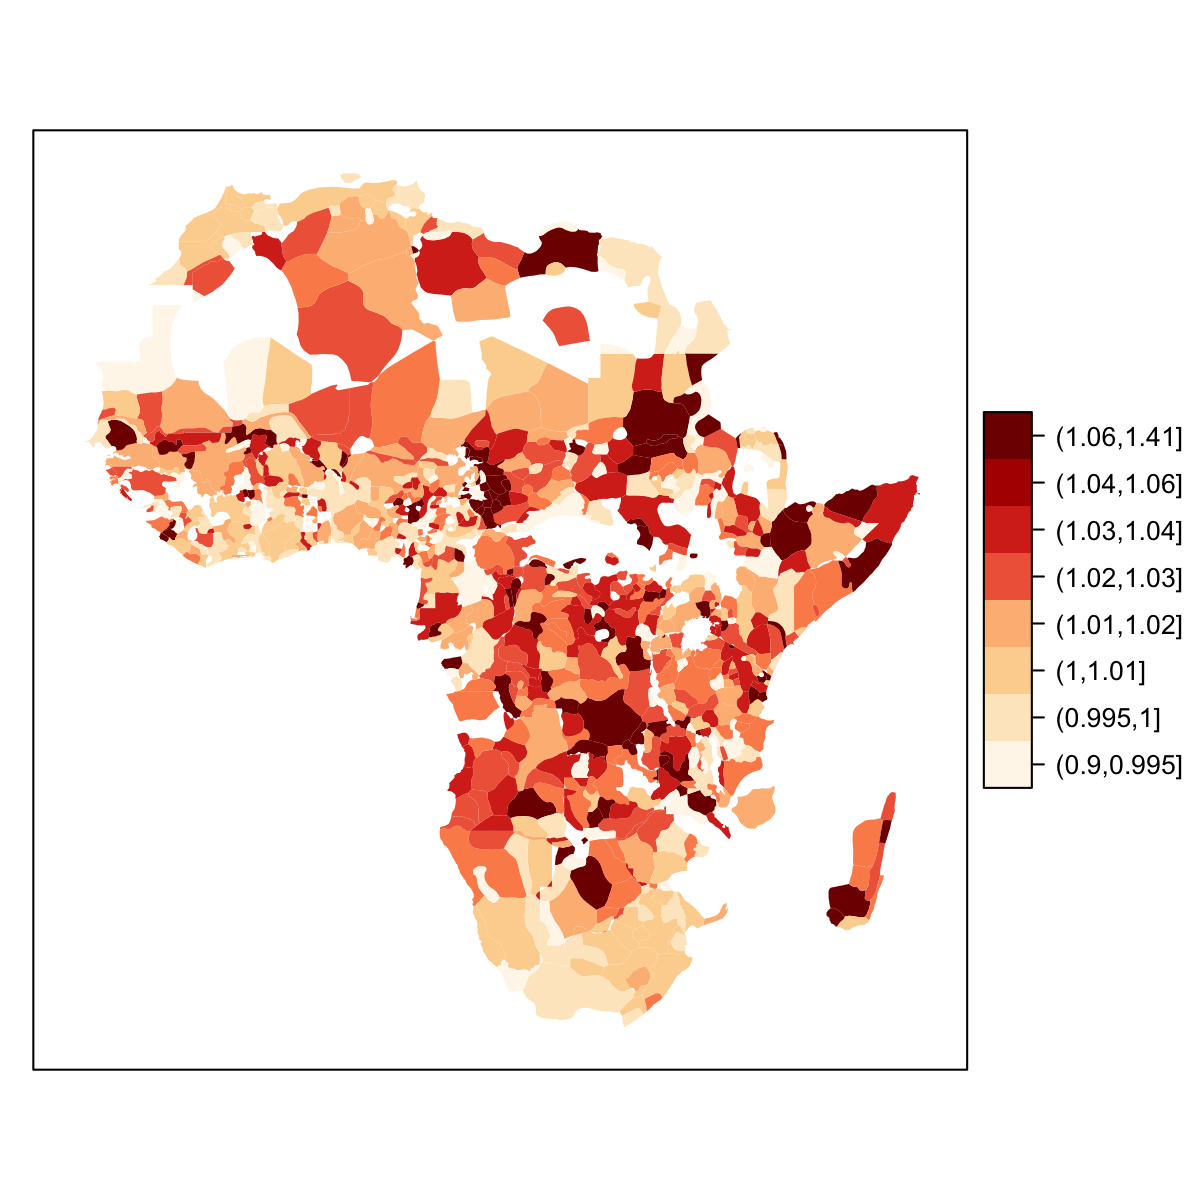
\includegraphics[width=0.65\textwidth,trim={1cm 4cm 0cm 4.5cm},clip]{../../Analysis/output/other_maps/ethnicity_zeta.png}


\label{fig:ethn_maps}
\mysubcaption{Spatial distribution of Local Infrastructure Discrimination Index $\Lambda_{h}$, aggregated over ethnic homelands. Unit of observation is pre-colonial homelands as initially defined in an ethnolinguistic map by \cite{Murdock_Africaitspeoples_1959} intersected by current political borders  \citep[following][]{Michalopoulos_LongRunEffectsScramble_2016}. $\Lambda_{h}$ is from grid cell level and weighted by population. Maps's colouring follows an equal-interval rule such that every colour in the spectrum has an equal amount of members. This is to visualise the measure's variation but leads to unequal bracket-sizes for each colour.}
\end{figure}
% End Figure

Using \citeauthor{Murdock_Africaitspeoples_1959}'s map on pre-colonial ethnolinguistic characteristics to identify current locations of ethnic homelands is not unproblematic. Firstly, the map originally appeared in small print in the appendix of \citeauthor{Murdock_Africaitspeoples_1959}'s book and was only later vectorised. When digitally scaling it up, the borders between homelands will naturally be subject to measurement error and imprecision \citep{Michalopoulos_PreColonialEthnicInstitutions_2013}. This should not be of much concern for the present study, as my underlying dataset on network inefficiency itself already only comes at a resolution of roughly 55 by 55 kilometres. The imprecise drawing of an otherwise detailed map arguably does not add much noise to my already noisy dataset (bearing in mind that the smallest homelands, which are most likely to be affected by drawing imprecision are automatically dropped from my dataset by way of constructing $\Lambda_{h}$, see above). Secondly, as \cite{Michalopoulos_PreColonialEthnicInstitutions_2013} point out, a map from 1959, reflecting homelands from the pre-colonial era, might not be an accurate representation of the current ethnic topography on the continent. It is reasonable to assume that people will have migrated away from their original ethnic homeland in a way that is endogenous to many of the (mainly development) variables I consider in this study. \cite{Nunn_SlaveTradeOrigins_2011} find that a majority of the continent's population still live in their ancestors' ethnic homelands, partially assuaging this concern. Moreover, I use \citeauthor{Murdock_Africaitspeoples_1959}'s map merely as a level of aggregation in order to gauge ethnic discrimination. Even if substantial migration patterns had taken place, it is still worthwhile to investigate whether governments treat homelands differentially based on their historic ethnic attribution.\footnote{Other than \cite{Michalopoulos_PreColonialEthnicInstitutions_2013,Michalopoulos_LongRunEffectsScramble_2016}, I do not make use of any of the auxiliary ethnolinguistic data provided in \citeauthor{Murdock_Africaitspeoples_1959}'s book. The definition of ethnic homelands is exclusively used to obtain an appropriate level of aggregation, not to characterise economic, societal, or institutional differences between them.} A final concern is that homelands are coded as non-overlapping, mutually exclusive regions. This conception does not leave room for diverse areas with multiple coexisting ethnicities. While this might be accurate for most rural areas, it is an untenably strong assumption for big, primal cities. Especially the capital city naturally attracts migrants from all parts of a country (and beyond), regardless of its immediately surrounding homeland. To counter this challenge, I follow \cite{Alesina_Ethnicinequality_2016} and exclude all ethnic homelands containing a country's capital city as a robustness check. As discussed below, this mostly does not alter results.

I investigate two patterns of infrastructure discrimination along ethnic lines, namely the preferential treatment of groups sharing the ethnic homeland with the national leader (\emph{ethnic favouritism}) and the negative treatment of groups excluded from the government (\emph{ethnic discrimination}). I begin with the latter. To measure ethnic discrimination, I rely on four measures of political relationships between ethnicities. Firstly, I make use of the Ethnic Power Relations (EPR) database by \cite{Vogt_IntegratingDataEthnicity_2015}, which globally identifies ``politically relevant ethnic groups and their access to state power'' \citep[p. 1328]{Vogt_IntegratingDataEthnicity_2015} over the past seven decades. Not every ethnic homeland inhabits a group that is ``politically relevant'', significantly truncating the sample by 46\%.\footnote{Merging EPR observations with ethnic homelands is non-trivial. Thankfully, I am able to rely on the conversion established by \cite{Michalopoulos_LongRunEffectsScramble_2016}.} EPR reports a yearly time series of political discrimination for every group in the sample. In particular, a group is coded as discriminated against by the central government if there is ``active, intentional, and targeted discrimination by the state against group members in the domain of public politics'' \citep[p. 1331]{Vogt_IntegratingDataEthnicity_2015}. As my dataset comes in the form of a simple cross-section without a time dimension, I follow \cite{Michalopoulos_LongRunEffectsScramble_2016} and analyse effects of a dummy variable taking on the value one if a group has experienced discrimination in at least one year between 1960 and 2010. I use this measure to investigate whether infrastructure discrimination covaries with political discrimination. Do groups which are actively discriminated in their political participation also see less than optimal trade investments in their homelands? Secondly, I broaden the definition of ethnic discrimination and more generally look at groups which are excluded from the central government. As defined by EPR, this classification entails all groups that are discriminated against (from above), plus groups that are defined as either powerless or self-excluded \citep[p. 1331]{Vogt_IntegratingDataEthnicity_2015}.\footnote{I again rely on the transformation by \cite{Michalopoulos_LongRunEffectsScramble_2016} who code an indicator as one if the ethnic group has experienced exclusion from the government at any point between 1960 and 2010.} Broadening the conception of ethnic discrimination allows for a more nuanced analysis of how non-access to power can influence network inefficiency. Thirdly, I analyse the effects of an EPR indicator denoting whether an ethnicity was part of a civil war with an explicitly ethnic dimension at some point between 1960 and 2010. The construction of this indicator is identical to the dummies described above and is obtained from \cite{Michalopoulos_LongRunEffectsScramble_2016}. As a more indirect measure for ethnic discrimination, I finally analyse whether ethnicities which were split in two or more parts by the arbitrary border drawings of the colonial powers get less than optimal infrastructure investment. \cite{Michalopoulos_LongRunEffectsScramble_2016} show that ethnic homelands of which ten or more per cent are in more than one country are significantly more prone to violence, have less political clout, and report less overall well-being.

To analyse patterns of infrastructure discrimination on the ethnic homeland level, I estimate a slightly different version of Equation \eqref{eq:grid_ols}
\begin{equation}
  \Lambda_{h,c} = \beta v_{h,c} + \textbf{X}_{h,c}\gamma + \delta_{c} + \epsilon_{h,c}
  \label{eq:ethn_ols}
\end{equation}
where $\Lambda_{h,c}$ is the Local Infrastructure Discrimination Index for homeland $h$ in country $c$, $\textbf{X}'_{h,c}$ and $\delta_{c}$ again denote controls and country fixed effects respectively, $v_{h,c}$ are the explanatory covariates discussed above, and $\beta$ is the coefficient of interest. The number of ethnicity observations (about 900) is significantly smaller than the number of grid cells. In order to avoid overfitting, I slightly truncate the set of controls $\textbf{X}'_{h,c}$. I replace the latitude and longitude polynomials, the classification into urban or rural, as well as dummies indicating proximity to a natural harbour, river, lake, and national border with two continuous measures of distance to the nearest border and distance to the coast. As homelands are much more irregularly shaped than grid cells, I also include the natural logarithm of each homelands' area \citep[as in][]{Michalopoulos_LongRunEffectsScramble_2016}. Apart from these adjustments, $\textbf{X}'_{h,c}$ entails all geographical and simulation controls of the models on the grid cell level. As many ethnicities appear more than once, the error term will reasonably be autocorrelated beyond the country-level. $\epsilon_{h,c}$ is hence plausibly not independent even across countries. To account for this, I follow \cite{Michalopoulos_LongRunEffectsScramble_2016} and double-cluster standard errors at both the country level as well as the ethnic family level using the mechanism proposed by \cite{Cameron_RobustInferenceMultiway_2011}.

% Figure Table Ethnic Discrimination
\begin{table}[t] \centering
  \caption{Null Effect of Ethnic Discrimination}
  \label{tab:Ethn_discrimination}
  \resizebox{\textwidth}{!}{


  \begin{tabular}{@{\extracolsep{5pt}}lcccccccc}
  \\[-1.8ex]\hline
  \hline \\[-1.8ex]
   & \multicolumn{8}{c}{\textit{Dependent variable: Local Infrastructure Discrimination Index $\Lambda_{h}$}} \\
  \cline{2-9}
  \\[-1.8ex] & (1) & (2) & (3) & (4) & (5) & (6) & (7) & (8)\\
  \hline \\[-1.8ex]
   Ethnicity discriminated against 1960--2010 & $-$0.001 & $-$0.001 &  &  &  &  &  &  \\
    \hspace*{3mm} \small (SE) & (0.008) & (0.007) &  &  &  &  &  &  \\
    \hspace*{3mm} \footnotesize \textit{[MDE]} & \textit{\footnotesize [0.021]} & \textit{\footnotesize [0.021]} &  &  &  &  &  &  \\
    & & & & & & & & \\
   Ethnicity excluded from the &  &  & $-$0.006 & $-$0.005 &  &  &  &  \\
    \hspace*{3mm} central government 1960--2010 &  &  & (0.005) & (0.005) &  &  &  &  \\
    &  &  & \textit{\footnotesize [0.014]} & \textit{\footnotesize [0.014]} &  &  &  &  \\
    & & & & & & & & \\
   Ethnicity involved in an &  &  &  &  & 0.002 & 0.002 &  &  \\
    \hspace*{3mm}  ethnic war 1960--2010 &  &  &  &  & (0.008) & (0.008) &  &  \\
    &  &  &  &  & \textit{\footnotesize [0.022]} & \textit{\footnotesize [0.022]} &  &  \\
    & & & & & & & & \\
   Ethnicity split by colonial borders &  &  &  &  &  &  & $-$0.002 & $-$0.002 \\
   &  &  &  &  &  &  & (0.004) & (0.004) \\
    &  &  &  &  &  &  & \textit{\footnotesize [0.011]} & \textit{\footnotesize [0.012]} \\
    & & & & & & & & \\
  \hline \\[-1.8ex]
  Country FE & Yes & Yes & Yes & Yes & Yes & Yes & Yes & Yes \\
  Geographic controls & Yes & Yes & Yes & Yes & Yes & Yes & Yes & Yes \\
  Simulation controls &  & Yes &  & Yes &  & Yes &  & Yes \\
  Observations & 496 & 496 & 496 & 496 & 496 & 496 & 932 & 932 \\
  R$^{2}$ & 0.156 & 0.166 & 0.158 & 0.168 & 0.156 & 0.167 & 0.164 & 0.167 \\
  \hline
  \hline \\[-1.8ex]
  \textit{Note:}  & \multicolumn{8}{r}{$^{*}$p$<$0.1; $^{**}$p$<$0.05; $^{***}$p$<$0.01} \\
  \end{tabular}

}

\mysubcaption{Statistically insignificant effects of various indicators of ethnic discrimination on the Local Infrastructure Discrimination Index $\Lambda_{h}$. The sample comprises ethnic homelands, projected on current national borders. Independent variable in columns (1)--(2) is a dummy variable indicating if an ethnicity has experienced discrimination from the government at some point between 1960-2010. In columns (3)--(4), independent variable is a dummy indicating if an ethnicity has been excluded from the central government at some point between 1960-2010. (5)--(6) analyse impacts of ethnicities being involved in a major ethnic war at some point between 1960--2010. All data gathered by \cite{Vogt_IntegratingDataEthnicity_2015} and obtained in transformed form from \cite{Michalopoulos_LongRunEffectsScramble_2016}. Explanatory variable in (7) and (8) is an indicator of ethnicities being split by national borders, defined as having at least 10 per cent of their homeland in more than one country \citep[from][]{Michalopoulos_LongRunEffectsScramble_2016}. Data for regressions in  (1)--(6) only exist for politically relevant ethnic groups, truncating the sample by 46\%. All observations exclude Western Sahara, for which no ethnic homeland data exist. Geographic controls consist of altitude, temperature, average land suitability, malaria prevalence, yearly growing days, average precipitation, indicators for the 12 predominant agricultural biomes, distances to the nearest coast and border, and the natural logarithm of the homeland area.  Simulation controls are comprised of population, night lights, and ruggedness. Results are robust to excluding homelands containing a country's capital (not reported). Heteroskedasticity-robust standard errors are double-clustered on the country level and the ethnic-family level and are reported in parentheses. All columns also report minimum detectable effect sizes (MDEs) in brackets. This is the smallest effect that would have still been detectable with 80\% power at 5\% significance \citep{Haushofer_ShorttermImpactUnconditional_2016}.}
\end{table}
% End Figure

Table \ref{tab:Ethn_discrimination} reports results of estimating Equation \eqref{eq:ethn_ols} for each of the four indicators of ethnic discrimination as independent variable. As before, the table prints estimates both with and without the set of simulation controls (consisting of population, night lights, and ruggedness). No estimate is significantly different from zero, implying that the null hypothesis of no linear relation between $v_{h}$ and $\Lambda_{h}$ cannot be rejected. There is no evidence suggesting that inefficiencies of the national trade network systematically covary with ethnicities that are historically discriminated against (columns 1--2), excluded from the government (3--4), involved in an ethnic war (5--6), or split by arbitrary colonial borders (7--8). Together, these results do not support the contention that discriminated ethnic groups are systematically disadvantaged in the design of national trade networks. After the social planner has reshuffled a country's roads, historically victimised groups are not better off than they were before. These (null) findings do not change when (a) excluding homelands containing a nation's capital, (b) including ethnic family fixed effects (c) controlling for pre-colonial differences in societal structure between ethnicities, namely complexity of hierarchies, the existence of compact settlement structures, and existence of a class system \citep{Michalopoulos_PreColonialEthnicInstitutions_2013}, (d) using a more lenient definition of split homelands whereby only 5\% of the territory has to be in more than one country (instead of 10\%), (e) clustering standard errors along merely (either) one dimension, and (f) excluding all geographic controls. All estimates hardly move and remain statistically indistinguishable from zero (not reported).

With null results, it can be a challenge to attribute the finding to there actually not being any underlying relationship in the data, or the study merely being underpowered to detect a reasonably sizeable effect. Especially, estimations in columns (1) -- (6) are performed on a substantially truncated sample compared to previous regressions and are hence prone to suffer from lack of statistical power. To gain an understanding for which of the two explanations is likely to account for the results at hand, I follow a recent contribution by \cite{Haushofer_ShorttermImpactUnconditional_2016} and calculate the \emph{Minimum Detectable Effect Size} (MDE) for each estimate. This is the smallest estimate that would have still been detectable with 80\% power at the 5\% significance level. As \cite{Haushofer_ShorttermImpactUnconditional_2016} demonstrate, the MDE can be computed as
\begin{equation*}
  \textrm{MDE} = (t_{1-\kappa}+t_{0.5\alpha}) \times SE(\hat{\beta})
\end{equation*}
where $SE(\hat{\beta})$ is the standard error of the estimated coefficient, and $t_{1-\kappa}=0.84$ and $t_{0.5\alpha}=1.96$ denote the values of the t-statistic required to achieve 80\% power and 5\% significance, respectively. This trivially simplifies to $\textrm{MDE} = 2.8 \times SE(\hat{\beta})$. I use this measure to gauge which order of magnitude my statistical tests are generally capable of detecting. If the MDE is very large, the underlying impact on $\Lambda_{h}$ would have to be substantial in order to even be noticed. Table \ref{tab:Ethn_discrimination} displays MDEs in brackets under each estimate's standard error. MDEs of ethnic discrimination and involvement in an ethnic war (columns 1--2 and 5--6) are slightly larger than $0.02$. This implies that victimising an ethnicity would have to lead to at least a 2\% increase (or reduction) in the Local Infrastructure Discrimination Index $\Lambda_{h}$ -- slightly larger effect sizes than being very close to a colonial railway (see Table \ref{tab:RailBlocks_zeta}). Considering the importance of ethnic power relations on subregional development in Africa, I regard this as a reasonably fine resolution. Minimum detectable effect sizes for ethnicities excluded from the government (columns 3--4) or split by colonial borders (7--8) are even smaller. The statistical tests are hence powered to detect even subtler effects. This leads to the conclusion that the reported null effects of Table \ref{tab:Ethn_discrimination} are not just an artefact of underpowered tests, but rather bolster the contention that active ethnic victimisation and trade network inefficiency are not systematically linked.

I also analyse the reverse effects of ethnic favouritism. Are ethnicities systematically better off when the country's leader was born in their homeland? Existing studies have shown that the rise to power of a new national leader leads to temporarily more consumption and output in the leader's birth region \citep{Hodler_RegionalFavoritism_2014} and ethnic homeland \citep{DeLuca_Ethnicfavoritismaxiom_2018}. During the leader's time in office, birth region and ethnic homelands also benefit from more foreign aid being channeled their way \citep{Dreher_AiddemandAfrican_2016}. \cite{Burgess_ValueDemocracyEvidence_2015} use a panel of public road expenditure in Kenyan districts over time and find that areas sharing the ethnicity of the current leader receive almost twice as much infrastructure spending and up to five times as many newly constructed road kilometres than the rest of the country. Remarkably, this ethnic bias attenuates in periods of democratic rule, providing evidence for the efficacy of inclusive political institutions in constraining patronage.

To investigate whether ethnic favouritism accounts for imbalances in trade infrastructure provision over space, I make use of a dataset of African national leaders provided by \cite{Dreher_AiddemandAfrican_2016}. The data entail information about the birth region and time in office of 117 heads of state holding power in 44 African countries dating back to 1969.\footnote{No data on national leaders are reported for Algeria, Western Sahara, South Sudan, Somalia, and Djibouti. Even for countries with data, coverage is not comprehensive as the dataset excludes leaders born abroad or with unknown birthplaces. 93.6\% of homelands never sent anyone to the highest office in the country. For those that did, tenures last from merely one year (the Zerma in Niger) to 42 years (the Duma in Gabon, homeland of long-term head of state Omar Bongo).} Using Open Street Map, I obtain coordinates for birthplaces and spatially merge them with my dataset on ethnic homelands. I then use this information to calculate for each ethnic group the total number of years someone born in the respective homeland has held high office. This allows me to analyse whether a homeland's over provision with transport infrastructure covaries with personal ties to national power.

Table \ref{tab:favoritism} investigates effects of ethnic and regional favouritism. Panel A, columns (1) through (5) estimate Equation \eqref{eq:ethn_ols} on the full sample of ethnic homelands intersected with current national borders. In (1) and (2), the explanatory variable is the total number of years someone born in the ethnic homeland was holding national power. The covariate enters with a significant and negative coefficient, implying that for each year one of their members was in power, an ethnic homeland is about 0.04 percentage points too well off given their relative position in the country's trade network. If the social planner were to intervene, she would strip the homeland with ethnic ties to power from some infrastructure and reallocate it towards areas with no such ties. The effect size is small -- with the median leader staying in power for nine years, ethnic favouritism distorts network efficiency in the order of magnitude of less than half a percentage point. Nevertheless, it provides further evidence for many of the recent findings on ethnic favouritism \citep{DeLuca_Ethnicfavoritismaxiom_2018}.


% Figure Table favoritism
\begin{table}[!t] \centering
  \caption{Ethnic and Regional Favoritism}
  \label{tab:favoritism}
  \resizebox{\textwidth}{!}{


  \begin{tabular}{@{\extracolsep{5pt}}lcccccccc}
  \\[-1.8ex]\hline
  \hline \\[-1.8ex]
   & \multicolumn{8}{c}{\textit{Dependent variable: Local Infrastructure Discrimination Index $\Lambda_{h}$}} \\
  \cline{2-9} \\[-1.8ex]
& \multicolumn{5}{c}{Full Sample} & \multicolumn{3}{c}{Excluding Capitals} \\
  \cline{2-6}   \cline{7-9}
  \\[-1.8ex] & (1) & (2) & (3) & (4) & (5) & (6) & (7) & (8)\\
  \hline \\[-1.8ex]
  \multicolumn{9}{l}{\textit{Panel A: Ethnicities}} \\
   Years in Power & $-$0.0004$^{**}$ & $-$0.0004$^{**}$ & $-$0.001$^{**}$ &  &  & $-$0.0003$^{*}$ & $-$0.0005$^{***}$ &  \\
  & (0.0002) & (0.0002) & (0.0003) &  &  & (0.0002) & (0.0002) &  \\
    & & & & & & & & \\
   Years in Power $\times$ Democracy  &  &  & 0.0004 &  &  &  & 0.0003 &  \\
  &  &  & (0.0003) &  &  &  & (0.0003) &  \\
    & & & & & & & & \\
   In Power Dummy &  &  &  & $-$0.007$^{*}$ & $-$0.008$^{**}$ &  &  & $-$0.007$^{*}$ \\
  &  &  &  & (0.004) & (0.004) &  &  & (0.004) \\
    & & & & & & & & \\
    Country FE & Yes & Yes & Yes & Yes & Yes & Yes & Yes & Yes \\
    Geographic controls & Yes & Yes & Yes & Yes & Yes & Yes & Yes & Yes \\
    Simulation controls &  & Yes & Yes &  & Yes & Yes & Yes & Yes \\
    Observations & 932 & 932 & 932 & 932 & 932 & 895 & 895 & 895 \\
    R$^{2}$ & 0.165 & 0.169 & 0.169 & 0.165 & 0.169 & 0.177 & 0.177 & 0.177 \\
   \hline \\[-1.8ex]
\multicolumn{9}{l}{\textit{Panel B: Grid Cells}} \\
  Years in Power & $-$0.001$^{***}$ & $-$0.001$^{***}$ & $-$0.001$^{***}$ &  &  & $-$0.001$^{***}$ & $-$0.001$^{**}$ &  \\
   & (0.0003) & (0.0002) & (0.0004) &  &  & (0.0003) & (0.0004) &  \\
   & & & & & & & & \\
  Years in Power $\times$ Democracy &  &  & $-$0.0001 &  &  &  & $-$0.0002 &  \\
   &  &  & (0.001) &  &  &  & (0.001) &  \\
   & & & & & & & & \\
  In Power Dummy &  &  &  & $-$0.024$^{***}$ & $-$0.025$^{***}$ &  &  & $-$0.026$^{***}$ \\
   &  &  &  & (0.006) & (0.006) &  &  & (0.007) \\
   & & & & & & & & \\

 Country FE & Yes & Yes & Yes & Yes & Yes & Yes & Yes & Yes \\
 Geographic controls & Yes & Yes & Yes & Yes & Yes & Yes & Yes & Yes \\
 Simulation controls &  & Yes & Yes &  & Yes & Yes & Yes & Yes \\
 Observations & 10,066 & 10,066 & 10,066 & 10,066 & 10,066 & 10,019 & 10,019 & 10,019 \\
 R$^{2}$ & 0.124 & 0.125 & 0.125 & 0.124 & 0.126 & 0.128 & 0.128 & 0.128 \\
 \hline
 \hline \\[-1.8ex]
 \textit{Note:}  & \multicolumn{8}{r}{$^{*}$p$<$0.1; $^{**}$p$<$0.05; $^{***}$p$<$0.01} \\
 \end{tabular}

}

\mysubcaption{Persistent impacts of holding power on Local Infrastructure Discrimination Index $\Lambda$ in leaders' homelands and birthplaces. Panel A estimates Equation \eqref{eq:ethn_ols} on the sample of ethnic homelands split by current national borders. Independent variable in columns (1)--(3) is the number of years since 1969 someone born in the homeland was the country's leader. Column (3) adds an interaction with a dummy indicating if the homeland is in a democratic country. In (4)--(5), the independent variable is a dummy indicating whether the homeland ever held power. Columns (6)--(8) replicate the regressions while excluding observations containing a country's capital. Panel B estimate Equation \eqref{eq:grid_ols} for similar models on the grid cell level. Data for leaders' birthplaces from \cite{Dreher_AiddemandAfrican_2016}, countries' democracy classification from \cite{Marshall_PolityProjectCenter_2015}. All observations exclude Western Sahara, for which no ethnic homeland data exist. Geographic controls consist of altitude, temperature, average land suitability, malaria prevalence, yearly growing days, average precipitation, indicators for the 12 predominant agricultural biomes. For ethnic homelands also distances to the nearest coast and border, and the natural logarithm of the homeland area. For grid cells also indicators for whether a cell is within 25 KM of a natural harbour, navigable river, or lake, the fourth-order polynomial of latitude and longitude, and an indicator of whether the grid cell lies on the border of a country's network. Simulation controls are comprised of population, night lights, ruggedness, and whether a cell is classified urban (for grid cells). Heteroskedasticity-robust standard errors are (double-)clustered on the country level (and the ethnic-family level for homelands) and are reported in parentheses.}
\end{table}
% End Figure


\cite{DeLuca_Ethnicfavoritismaxiom_2018}, \cite{Hodler_RegionalFavoritism_2014}, and \cite{Burgess_ValueDemocracyEvidence_2015} have hypothesised that ethnic favouritism is less prevalent in more democratic countries, especially on the African continent. To test for similar patterns in my setting, I follow \citeauthor{DeLuca_Ethnicfavoritismaxiom_2018} and interact total years in power with a variable capturing democratic institutional quality, as reported by \cite{Marshall_PolityProjectCenter_2015}. The variable comes from the Polity4 project and ranks each country on a scale from -10 (authoritarian) to 10 (democratic). I transform this score to a dummy equalling one if a country had a positive rating in 2016. Column (3) reports results of estimating equation \eqref{eq:ethn_ols} including an interaction term.\footnote{The equation to be estimated is \begin{equation*}
  \Lambda_{h,c} = \beta_{1} YearsInPower_{h,c} + \beta_{2} YearsInPower_{h,c}\times Democracy_{h,c} + \textbf{X}_{h,c}\gamma + \delta_{c} + \epsilon_{h,c}
\end{equation*} with the country fixed effect capturing any ex-ante difference between countries' score in $Democracy_{h,c}$.} The coefficient for the number of years in power is strongly attenuated, yet remains significant at the 5\% level. Contrarily, the interaction term enters with an estimate not significantly different from zero. Countries that were democratic in 2016 are not performing better or worse in curtailing ethnic favouritism.

After having analysed intensive margin effects of the number of years in power, columns (4) and (5) extend the inquiry to the extensive margin. The explanatory variable is now a dummy equalling one if an ethnic homeland has ever had someone represent them as head of state (regardless of how long). The coefficient enters significantly and negatively, implying that ethnic favouritism is not constrained to a few long-term national leaders.

The regressions of Table \ref{tab:favoritism} are not perfectly identified. While I do control for an extensive set of auxiliary variables, unobservable differences between homelands might still simultaneously impact both their infrastructure provision, as well as their chances of sending some of their own to be national leader. This bias is particularly evident for national capitals: leaders disproportionally are born in the capital, and capitals also have significantly better infrastructure provision. To try to account for this confound, I re-estimate columns (2), (3), and (5) while excluding all homelands which include a nation's capital. Results are printed in columns (6) -- (8) and are not qualitatively different from the full sample estimates. Significance becomes slightly weaker in (6) and (8), yet slightly stronger in (7). The effect thus prevails even in homelands not geographically connected to the places of power.

Regional favouritism, the notion that a leader would disproportionally channel government resources towards his or her birthplace (rather than ethnic group), has been a competing hypothesis to favouritism on ethnic grounds. I explore this potential source of network inefficiency in Panel B of Table \ref{tab:favoritism}. Again using the dataset by \cite{Dreher_AiddemandAfrican_2016}, I identify birthplaces of national leaders and assign them to individual grid cells. The 10,000+ cells are on average much smaller than ethnic homelands and hence allow to detect preferential treatment on a much more confined regional scale. The exposition of columns (1) through (8) immediately follows Panel A, yet the set of controls is slightly altered to match the grid cell level strategy of the rest of this study.\footnote{As with all regressions on the grid cell level, Equation \eqref{eq:grid_ols} is estimated, full geographic and simulation controls are included, and standard errors are clustered solely along the country dimension.} Results are similar to Panel A, yet much stronger. Per year someone born in a given grid cell held the country's highest office, the cell has 0.1 percentage points too much welfare compared to the social optimum (columns 1--2). The premium of ever sending someone to the highest office is estimated at 2.5 percentage points (column 5) -- an effect equivalent to the difference between a cell without any colonial railroads and the cell with the highest total amount of railway kilometres in Africa. These estimates do not change when allowing for differentiation by democratic institutions (column 3) or excluding all grid cells containing a capital (6--8). Taken at face value, the results strongly suggest the presence of regional favouritism distorting the spatial optimum of African trade networks.

As alluded to above, the estimations of Table \ref{tab:favoritism} are notoriously afflicted with endogeneity concerns. Even after controlling for many immediate confounds like population, economic activity, geographical characteristics, or country fixed effects, one cannot rule out that areas producing a national leader are still substantially different along unobservables. Hard-to-quantify idiosyncrasies like an area being a historical party stronghold or having been of strategic importance in a military coup which produced a new head of state might lead to disproportionally many leaders from a certain region, while also explaining differential infrastructure investments into the area. Incapable of conducting a large scale experiment and randomly allocating leadership positions to arbitrary members of society, most of the well-identified studies on ethnic or regional favouritism solve the endogeneity problem by introducing a time dimension. \cite{DeLuca_Ethnicfavoritismaxiom_2018}, \cite{Burgess_ValueDemocracyEvidence_2015}, and \cite{Hodler_RegionalFavoritism_2014} all fit panel equations with region fixed effects, accounting for any ex-ante differences between areas. They hence isolate the effect of preferential treatment \emph{while in office}. Since my dataset comes as a mere cross-section, I can only investigate effects of favouritism which might have occurred \emph{at any time in the past}.\footnote{There have been studies attempting to isolate the relationship without a time dimension. \cite{Soumahoro_LeadershipfavouritismAfrica_2015} regresses current night lights on past leadership tenures without a panel and finds a very strong effect. These results have been deemed vastly too large by the subsequent literature which had the luxury of including time fixed effects. I interpret this as further evidence for heterogeneity along unobservables, potentially confounding a simple cross section and affecting my results.} While this data limitation clearly dilutes the robustness of my findings, it is worth bearing in mind that my outcome variable has a different interpretation to most of the studies above. Existing research designs analyse variations in flow variables like annual night lights or government expenditures, yet my measure of network inefficiency is a stock variable. As infrastructure is highly persistent, $\Lambda$ encapsulates information about innumerable transport investment decisions made in the past. If a leader was in power for only a short period in the 1990s, but used the time in office to heavily cater to his or her birth region, one would still expect to see traces of this behaviour in the current infrastructure discrimination index. Regressing current network outcomes on past leadership tenures is hence worthwhile. As I cannot fully rule out the confounding power of unobservables, however, the results of Table \ref{tab:favoritism} should be taken with a grain of salt.\footnote{I can quantify the distorting power unobservables would need to have in order to wash away the entire effect with the technique proposed by \cite{Altonji_SelectionObservedUnobserved_2005}. Using the result without simulation controls in column (1), Panel B, Table \ref{tab:favoritism} as restricted sample estimate $\widehat{\beta^{R}}$ and the one with simulation controls (column 2) as full sample estimate $\widehat{\beta^{F}}$, I can gauge how many times more I would have to introduce a control set equally powerful in order to attenuate all of the detected relationship. With the derivation by \cite{Nunn_SlaveTradeOrigins_2011}, this is easily computed as $\widehat{\beta^{F}}/(\widehat{\beta^{R}}-\widehat{\beta^{F}})$. With the given estimates in Table \ref{tab:favoritism}, I obtain a measure of 124.9. In other words, I would have to be unaware of unobservables 125 times as powerful as the additional controls added in column (2) -- night lights, population, urban characteristics, and ruggedness -- in order to falsely detect an effect where there is none. As these are fundamental determinants of economic activity, it is unlikely that unobservables of similar magnitude still exist. While this might sound promising, it is worth noting that the literature has recently warned against relying too much on such tests, especially in environments with much unexplained variation and low $R^{2}$ values \citep[see][]{Oster_UnobservableSelectionCoefficient_2018}.}

Ethnic and regional favouritism are not mutually exclusive. A leader can channel government resources towards inefficient infrastructure projects in both his or her ethnic homeland, as well as distinct birth region. Indeed, by way of constructing the indicators, a leader's birthplace is always contained within his or her ethnic homeland, complicating efforts to distinguish between the two effects. As a first attempt, I also construct a measure of network inefficiency on the homeland level \emph{excluding} the one grid cell in which a leader was born. I obtain this by cutting each rectangular birthplace cell out of the much bigger homeland areas and aggregating over this newly constructed polygon, as proposed by \cite{DeLuca_Ethnicfavoritismaxiom_2018}. When replicating Panel A of Table \ref{tab:favoritism} with this newly created measure as dependent variable, all estimates turn insignificant (see appendix, Table \ref{tab:APP:favoritism_sans}). While this might naïvely be interpreted as evidence that favouritism does not extend beyond small birth regions, one has to again be cautious of censoring the dependent variable in such a way. If birth regions are inherently different, cutting them out biases estimates on the remaining sample. With the existing data, I am unable to clearly attribute the effects to one of the two explanations.

In this section, I have investigated how ethnic relations skew trade networks towards a sub-optimal state. While I did not find any evidence suggesting that vulnerable and victimised groups are systematically disadvantaged by the current trade system, I descriptively showed that the reverse is true -- ethnicities and regions which have one of their members hold national power are too well off given their relative position in the network. I have presented evidence that this premium exists for both large ethnic homelands and locally confined birth places and is not attenuated in democratic governments. Further research is needed to clearly distinguish between the two.

\subsection{Foreign Aid}
Africa is the primary target of international aid. In 2017, no other world region was awarded more development disbursements from The World Bank -- indeed, African countries received more aid than Europe, Central Asia, Latin America, and the Caribbean combined \citep{TheWorldBank_WorldBankAnnual_2017}. Of almost 12 billion US dollars worth of lending commitments, the biggest share was awarded to projects aimed at improving transportation infrastructure.\footnote{The transport sector made up 18\% of total IBRD and IDA lending to African nations, followed by water and sanitation (14\%), energy and extractives (14\%), and public administration (12\%) \citep{TheWorldBank_WorldBankAnnual_2017}.} The World Bank is not alone -- in the past decade, non-traditional players have entered and disrupted the international development aid system \citep{Dreher_Rogueaidempirical_2015}. Most notably, China has emerged as a significant donor nation, funding development projects in at least 50 African countries since the turn of the millennium \citep{Strange_TrackingUnderreportedFinancial_2017}.

Despite the vast amount of resources involved, foreign aid has not yet been unequivocally proven to be linked with positive economic outcomes in recipient countries. An influential literature has long debated whether aid leads to economic growth on the country level \citep{Burnside_AidPoliciesGrowth_2000,Easterly_AidPoliciesGrowth_2004,Rajan_Aidgrowthwhat_2008}. Plagued with data shortcomings and identification challenges, the discourse remained inconclusive for years, up to a point where frustrated researchers were even calling into question the very merit of the entire research agenda \citep{Clemens_CountingChickenswhen_2012,Clemens_NewRoleWorld_2016}. New advances in geo-referenced data availability \citep{Dreher_Aidgrowthregional_2015,Dreher_AidChinaGrowth_2017} and instrumentation techniques \citep{Nunn_USFoodAid_2014,Clemens_CountingChickenswhen_2012} have since reignited the literature on the effects of foreign aid.

How do development aid projects relate to my measure of inefficient trade networks? Since the United Nations summarise international aid efforts as aiming to 'leave no one behind' \citep{Briggs_LeavingNoOne_2018} and The World Bank pledges to eradicate extreme poverty \citep{Clemens_NewRoleWorld_2016}, one could expect international aid projects to disproportionally target areas that are discriminated against. Places that have less than they deserve should receive more attention from development agencies. For transport projects in particular, international donor organisations could be expected to play a role similar to the social planner in my infrastructure reallocation exercise. If a region has more roads than socially optimal, The World Bank should ideally devise new infrastructure projects elsewhere. To this end, it is worthwhile to investigate to what extent foreign transport aid achieves to promote overall network efficiency on the African continent.

The prime challenge to address when conducting empirical investigations into the spatial distribution of development assistance is obvious threats to identification. Decisions on where to place a foreign aid project are notoriously \emph{not} exogeneous. Large foreign lending lines are allocated to potential project sites based on expectations about maximum impact in furthering development objectives. In this, fund placement is inherently non-random. The World Bank, for example, accountable to its donors and member countries, operates large monitoring, evaluation, and research departments with the objective to take unwanted arbitrariness out of the aid allocation process \citep{Banerjee_EvaluationWorldBank_2006}. While certainly laudable and necessary, this complicates isolating causal effects of spatial differences in aid placement. The direction of the arising bias is ex-ante ambiguous. Areas which receive development assistance might be in particularly exigent need, rendering them incomparable to areas that do not receive much aid. Then again, donor institutions might also seek to target regions which are expected to grow anyway in order to accelerate the process. There are two strategies to deal with this empirical challenge. On the one hand, a large literature has relied on instrumentation techniques in attempts to isolate plausibly exogeneous parts of the spatial variation in aid. Research designs have harnessed idiosyncrasies in bilateral relations between donor and recipient countries \citep{Rajan_Aidgrowthwhat_2008}, exogeneous shocks to domestic commodity production in donor nations \citep{Nunn_USFoodAid_2014,Dreher_AidChinaGrowth_2017}, or the crossing of plausibly arbitrary thresholds for aid eligibility \citep{Galiani_effectaidgrowth_2017}. A second approach, however, is to just acknowledge the underlying endogeneity of aid placement and even render it the object of inquiry. This \emph{aid targeting} research agenda does not aim to identify causal effects of development assistance, but merely seeks to evaluate who gets what based on a vector of observable characteristics. Contributions to this literature have investigated political considerations \citep[e.g.][]{Dreher_Rogueaidempirical_2015}, long run persistence \citep{Alpino_LightingPathInfluence_2017}, or fund embezzlements \citep{Dreher_AiddemandAfrican_2016} as potential confounds of optimal targeting.

To investigate whether international development aid is quantitatively associated to my measure of trade network inefficiency, I make use of two recently established datasets of geo-referenced aid flows to Africa. Firstly,  \cite{AidData_WorldBankGeocoded_2017} in cooperation with The World Bank, tracks over 5,600 lending lines from The World Bank to African nations and reports precise coordinates of over 60,000 projects financed through these funds, totalling more than 300 billion US dollars. The sample comprises all projects approved between 1996--2014. As \cite{Strandow_UCDPAidDataCodebook_2011} describe, attributing projects to locations relies on a double-blind coding procedure of various World Bank documents. Secondly, I explore patterns from a  similar database on Chinese aid projects by \cite{Strange_TrackingUnderreportedFinancial_2017}. The motivations behind China's involvement in Africa are opaque and data on aid flows are much less transparent than from traditional donors, rendering precise, geo-referenced attribution much more cumbersome. \citeauthor{Strange_TrackingUnderreportedFinancial_2017} resort to reports from numerous local and international media outlets to track official and unofficial financing lines to over 1,500 projects worth 73 billion US dollars in the period 2000--2011. As \citeauthor{Strange_TrackingUnderreportedFinancial_2017} point out, media reports are often based on initial press releases and do not necessarily follow up on the eventual disbursement of every promised dollar. In that, the dataset is likely to capture Chinese funding \emph{commitments} rather than actual \emph{disbursements}. Insofar as donors usually commit to more than they eventually deliver, these figures present an upper bound of realised development assistance. Furthermore, while \cite{AidData_WorldBankGeocoded_2017} claim their dataset on World Bank projects to be exhaustive, the dataset on Chinese aid will naturally miss some unofficial flows, as significant parts of Chinese involvement remain untracked.

% Figure Maps of Aid
\begin{figure}[t]
\centering
\caption{Spatial Distribution of Development Aid Projects to African Nations}

\begin{subfigure}[c]{0.48\textwidth}
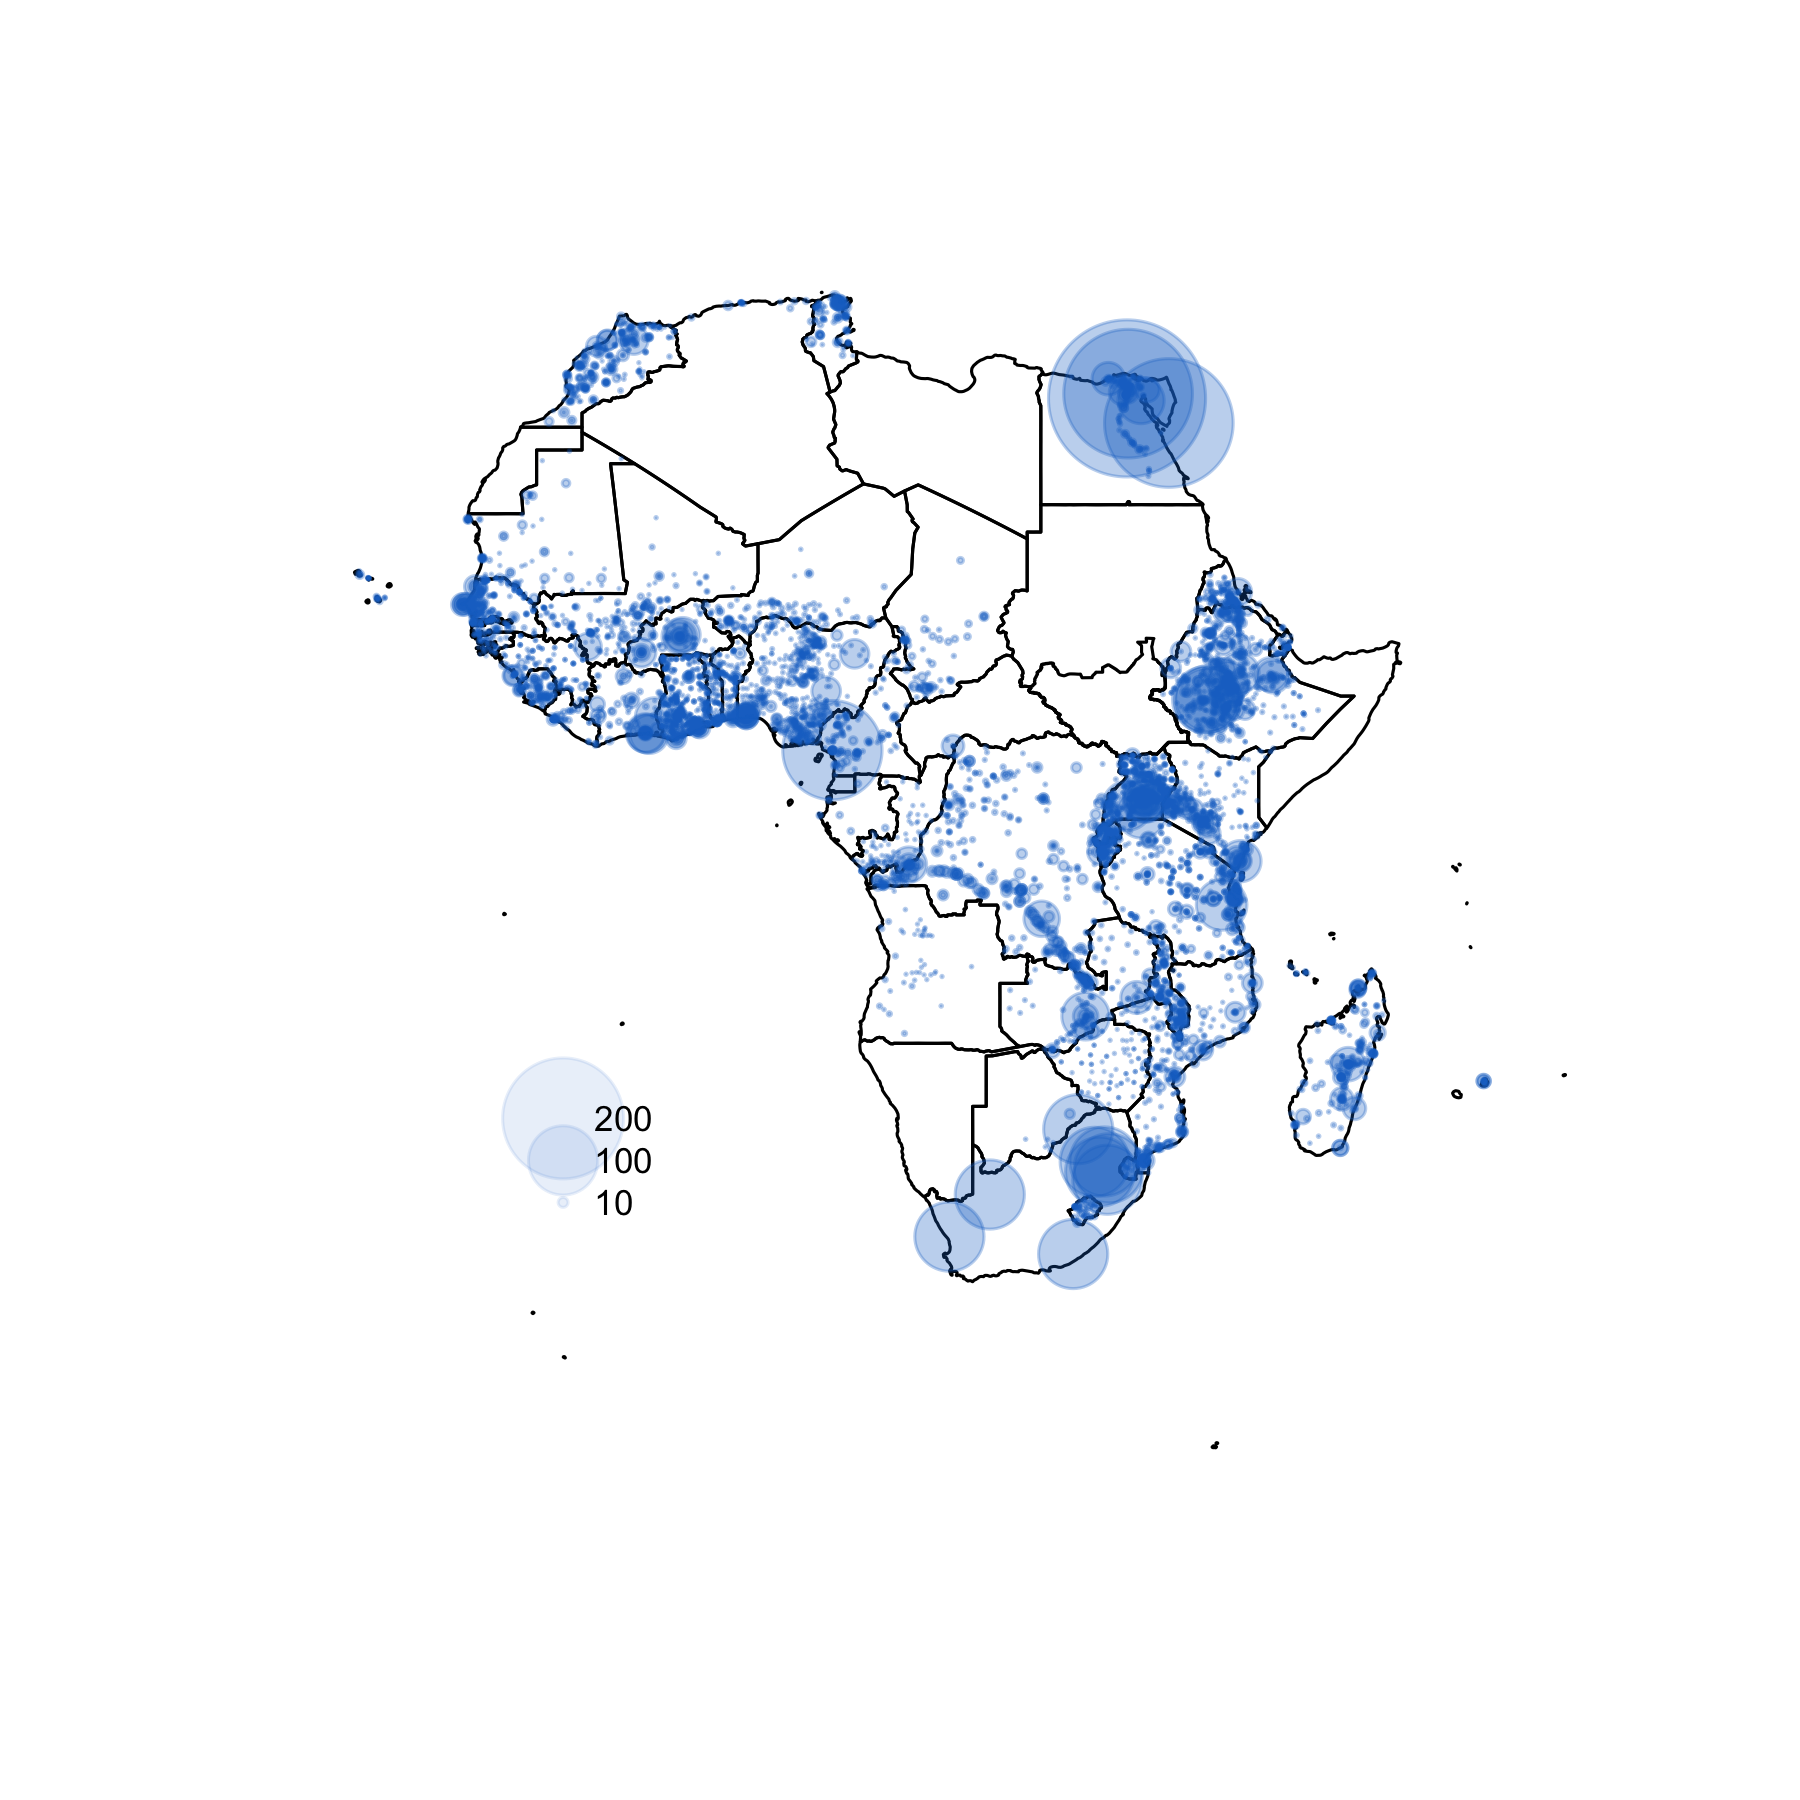
\includegraphics[width=\textwidth,trim={15cm 16cm 10cm 8cm},clip]{../../Analysis/output/other_maps/aid_wb.png}
\caption{World Bank Aid}
\label{fig:WB_aid_map}
\end{subfigure}
\begin{subfigure}[c]{0.48\textwidth}
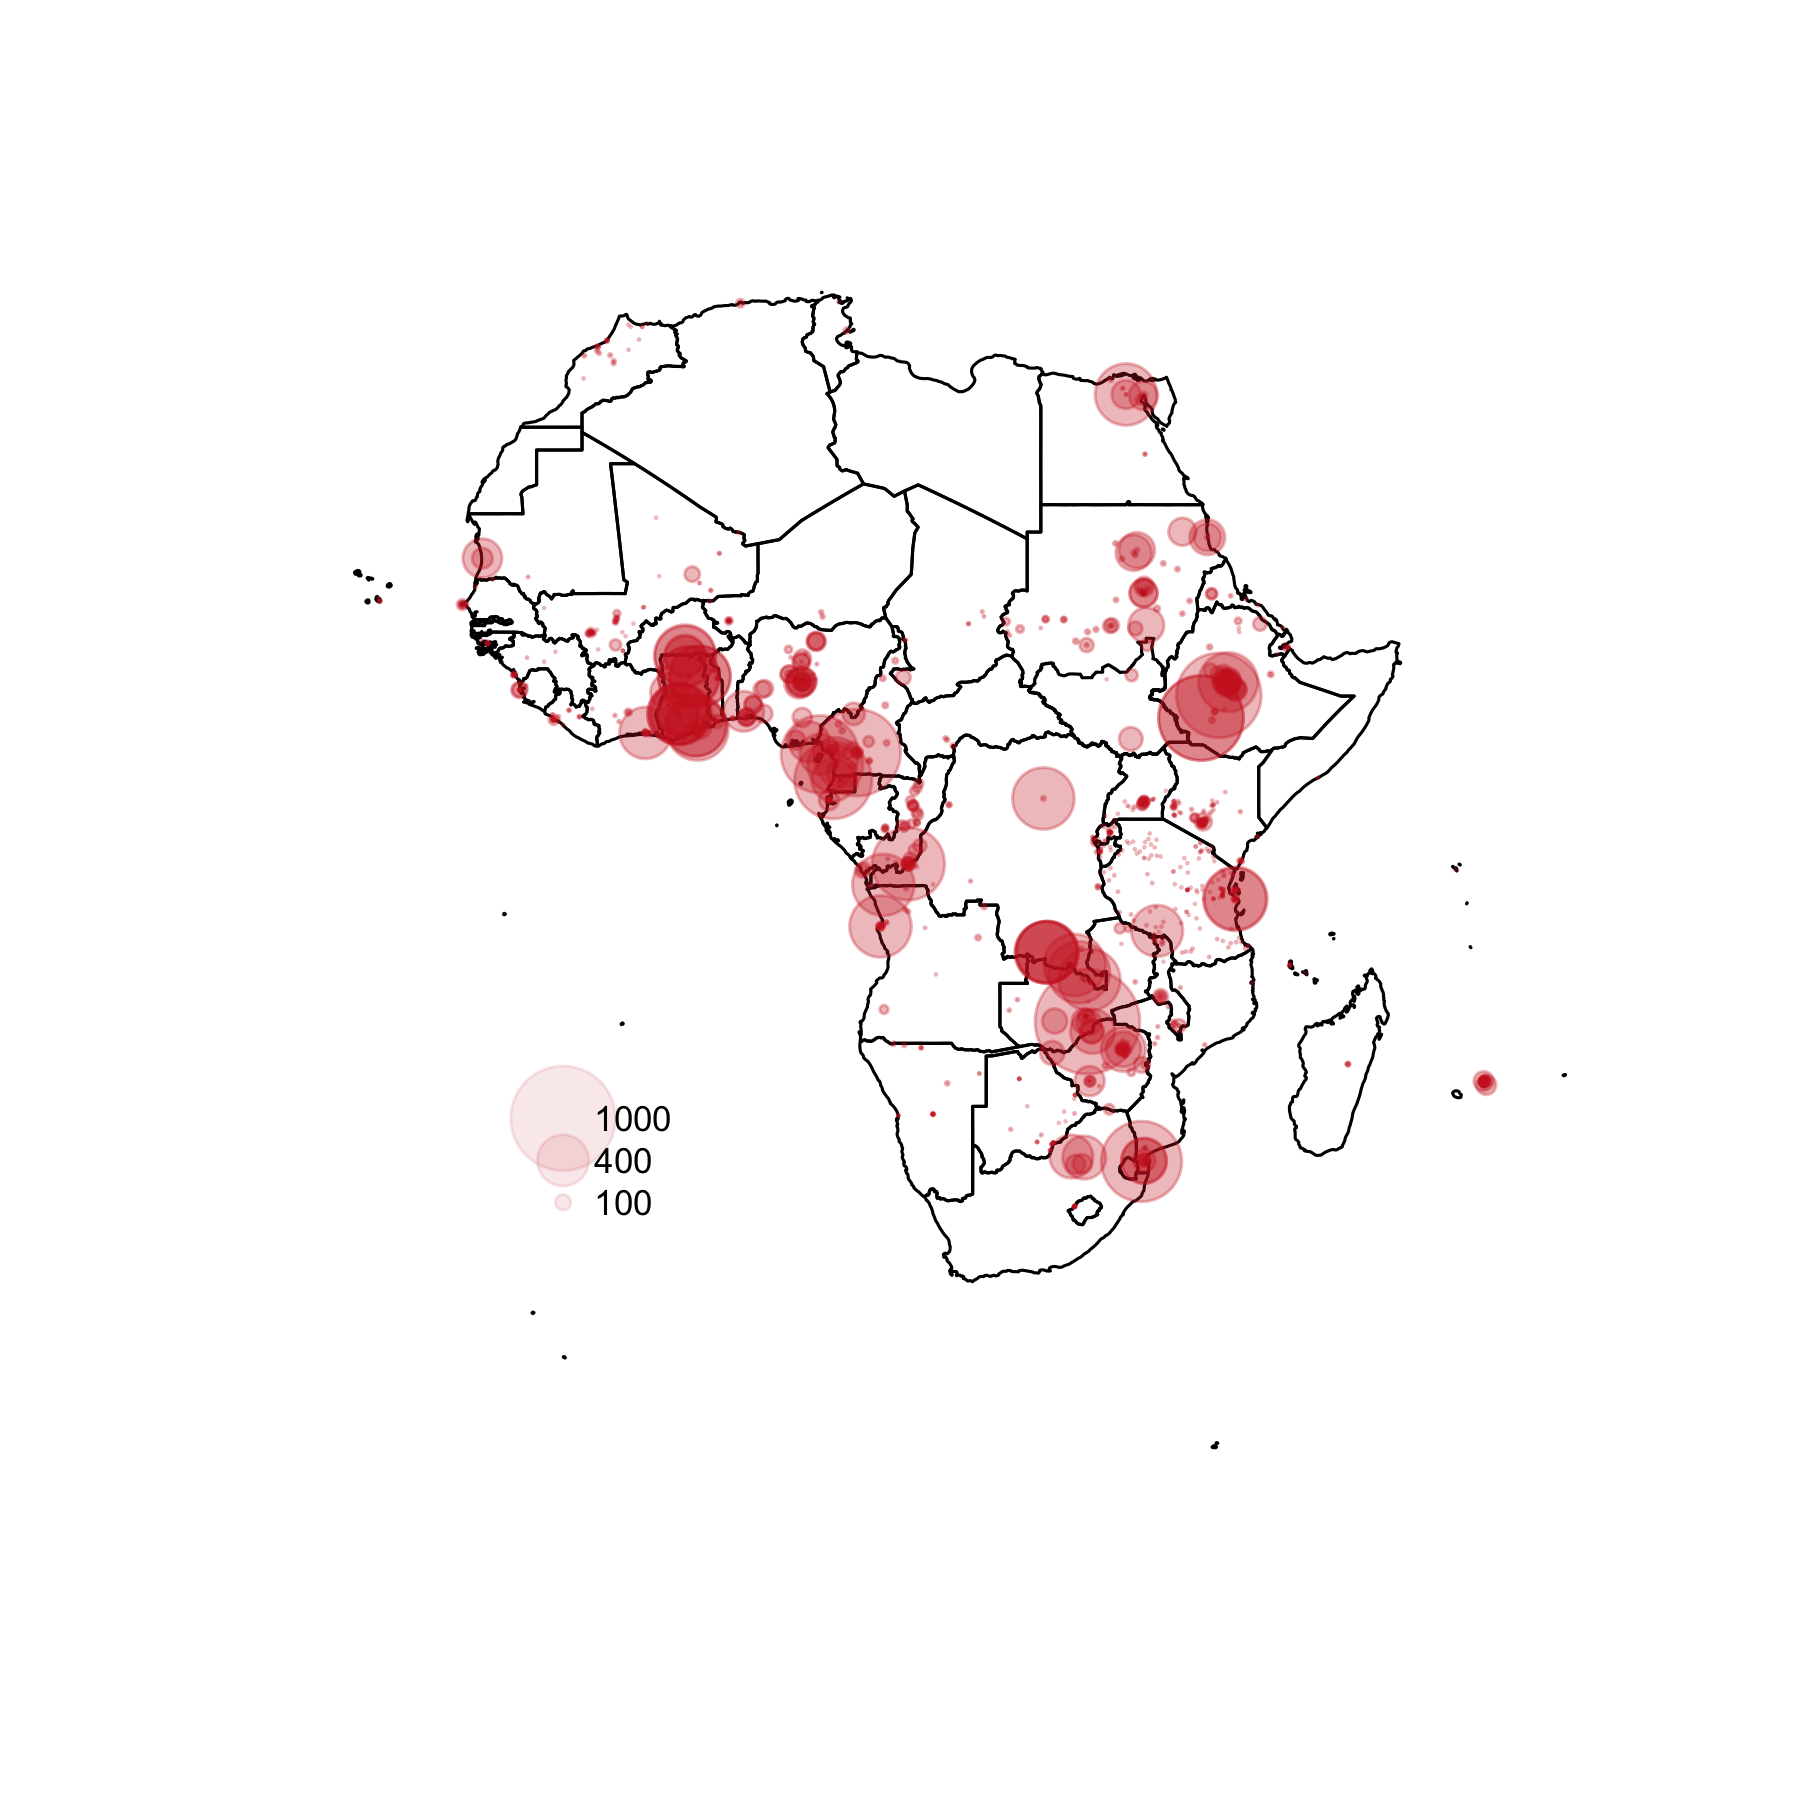
\includegraphics[width=\textwidth,trim={15cm 16cm 10cm 8cm},clip]{../../Analysis/output/other_maps/aid_China.png}
\caption{Chinese Aid}
\label{fig:China_aid_map}
\end{subfigure}

\label{fig:Aid_maps}
\mysubcaption{Foreign aid projects funded by The World Bank \eqref{fig:WB_aid_map} and China \eqref{fig:China_aid_map}. Each dot represents one project site with radius proportional to the logarithm of total disbursements flowing to each site. World Bank data comprise all projects approved between 1996--2014. Chinese data include tracked projects between 2000--2011. Map only depicts projects coded with sufficient precision to not be excluded (see text). If a project has multiple sites, total disbursements are assumed evenly distributed between locations. Data from \cite{AidData_WorldBankGeocoded_2017} and \cite{Strange_TrackingUnderreportedFinancial_2017}. Legend denotes disbursement values in million 2011 US dollars. Note that the legends have different scales.}
\end{figure}
% End Figure

For the purpose of this study, I exclude aid projects with no clear-cut geographical target like unconditional lending lines to the central government or assistance for political parties. I also exclude flows with unknown or only vague information on eventual project location.\footnote{Specifically, I exclude all projects with a precision code of more than 3 -- this corresponds to projects only identified at province-level or above. The remaining entries are geo-coded either exactly (61\%), within a 25 kilometre radius (4\%), or with municipality-level precision (35\%) \citep{Strandow_UCDPAidDataCodebook_2011}.} I also ignore projects which were still under construction or otherwise not fully completed by the end of 2017 (when I was scanning the Open Street Map database for road data). Together, these steps truncate the World Bank sample by 35\% and the China sample by 52\%. In Figure \ref{fig:Aid_maps}, I map the spatial distribution of aid projects from both remaining samples. Each circle represents a project site, with radius proportional to (log) US dollar disbursement value.\footnote{All disbursements are adjusted to 2011 US dollars. For projects with multiple sites, I assume total disbursement value to be split evenly between sites.} Inspecting Subfigure \ref{fig:WB_aid_map}, a remarkable degree of geographical clustering of World Bank aid provision becomes apparent. Some countries like Namibia, Somalia, or both Sudans have not received any local World Bank development assistance, while efforts to speed up civil war recovery have made Uganda and Rwanda primary targets for Bank funding. Chinese assistance in \ref{fig:China_aid_map} is naturally more sparse, yet on average comprised of more voluminous projects. Furthermore, China also achieves fairly comprehensive coverage of almost all African subregions. As \cite{Strange_TrackingUnderreportedFinancial_2017} point out, the only ominous omissions from the Chinese aid portfolio pertain to Burkina Faso and Swaziland, countries that officially recognise the Republic of Taiwan.

In order to analyse spatial relationships between foreign aid and my measure of local network inefficiency, I aggregate the total value of aid disbursements from the remaining 10,786 World Bank projects and 1,420 Chinese projects onto the grid cell level. Of the 10,158 grid cells of my sample, more than 21\% have received some form of assistance from either source. On average, these cells receive aid volumes of more than 30 million US dollars. The area receiving the most total World Bank funding is the grid cell containing Uganda's capital Kampala, which saw more than 380 million US dollars flowing its way. The Bank has funded the area with a vast power sector development project spanning four sites in the cell, which was finished in 2011. A large environmental effort for sustainable development in the Lake Victoria region also falls in this grid cell. The biggest beneficiary of Chinese development assistance is a grid cell in the south of Congo-Kinshasa, where Chinese funds of almost 5 billion US dollars helped construct a vast copper mining infrastructure, including four mines and an extensive railway and road system to connect the sites to the global market.\footnote{As \cite{Strange_TrackingUnderreportedFinancial_2017} report, financing was realised as a loan agreement on concessionary repayment terms. This megaproject was initially even devised at up to 9 billion USD, however the IMF voiced concerns about the mounting debt of the DRC and the deal was scaled down. In Subfigure \ref{fig:China_aid_map}, other projects at first glance seem to be bigger. However, note that this copper project is showing up as multiple sites at very close distance from each other in the dataset. On the map, they overlap.}

Do donor institutions identify places most in need of additional infrastructure? I employ various indicators of aid provision in the standard grid cell level framework based on Equation \eqref{eq:grid_ols}. I rely on two measures to quantify the prevalence of foreign aid: the total value of aid disbursements to a grid cell in 2011 US dollars and the number of distinct project sites within a given cell. This distinction is useful to capture effects on both intensive and extensive margins. As \cite{Dreher_Aidgrowthregional_2015} point out, extensive margin effects might be driven by the presence of development advisory and consultancy services, which go beyond the mere volume of a given project. I analyse World Bank and Chinese funds separately to account for the different methodologies used to create the two databases. I also put additional emphasis on infrastructure by separately analysing variation in funds going only to infrastructure projects in the transportation sector.

Table \ref{tab:Aid_Baseline} reports results. Panel A investigates the spatial distribution of World Bank assistance. The estimates reveal seemingly opposing objectives between the Bank and the social planner. Recall that if the objectives were aligned, World Bank aid would go into regions which also stand to gain under the efficient reallocation exercise. In other words, funds should flow towards areas that are discriminated against and have high $\Lambda_{i}$ values. Instead, the opposite seems to be true. Negative estimates in columns (1) and (2) reveal that grid cells receiving more World Bank assistance score lower on the Local Infrastructure Discrimination Index $\Lambda_{i}$. These are areas the social planner identifies as overly privileged. Indeed, every additional million US dollar flowing into an area is associated with the grid cell being about $0.04$ percentage points too well off, even after adjusting for geography, population, and economic activity, and only analysing within-country variation (column 2). Were the social planner to intervene and reallocate infrastructure, she would systematically take roads and welfare away from cells which received more World Bank funding. Columns (3) and (4) zoom in on this dynamic and only analyse funds going to 2,949 transport infrastructure projects. This is to rule out that the effects of (1)--(2) are driven by other types of World Bank assistance. Results are qualitatively similar, yet much stronger. The average transport infrastructure project size of around 3 million US dollars goes to grid cells which stand to lose $0.3$ percentage points of welfare under the reallocation exercise. Similar effects hold on the extensive margin reported in columns (5)--(8). More project sites are associated with regions judged too well off by the social planner, regardless of whether the focus lies on assistance in general (5--6), or more specifically transportation infrastructure projects (7--8).

% Figure Table Aid Baseline
\begin{table}[!t] \centering
  \caption{Foreign Aid Projects}
  \label{tab:Aid_Baseline}
  \resizebox{\textwidth}{!}{


  \begin{tabular}{@{\extracolsep{5pt}}lcccccccc}
  \\[-1.8ex]\hline
  \hline \\[-1.8ex]
   & \multicolumn{8}{c}{\textit{Dependent variable: Local Infrastructure Discrimination Index $\Lambda_{i}$}} \\
  \cline{2-9}
  \\[-1.8ex] & (1) & (2) & (3) & (4) & (5) & (6) & (7) & (8)\\
  \hline \\[-1.8ex]
  \multicolumn{9}{l}{\textit{Panel A: Worldbank Projects}} \\
  \\[-1.8ex]
  Total disbursements & $-$0.0003$^{***}$ & $-$0.0004$^{***}$ &  &  &  &  &  &  \\
  \hspace*{3mm} in million 2011 US dollars & (0.0001) & (0.0001) &  &  &  &  &  &  \\
   & & & & & & & & \\
  Transport-sector disbursements &  &  & $-$0.001$^{***}$ & $-$0.001$^{***}$ &  &  &  &  \\
   \hspace*{3mm} in million 2011 US dollars &  &  & (0.0002) & (0.0002) &  &  &  &  \\
   & & & & & & & & \\
  Number of projects &  &  &  &  & $-$0.002$^{***}$ & $-$0.003$^{***}$ &  &  \\
   &  &  &  &  & (0.0004) & (0.0004) &  &  \\
   & & & & & & & & \\
  Number of transport projects  &  &  &  &  &  &  & $-$0.003$^{***}$ & $-$0.004$^{***}$ \\
   &  &  &  &  &  &  & (0.001) & (0.001) \\
   & & & & & & & & \\
\\[-1.8ex]
 Country FE & Yes & Yes & Yes & Yes & Yes & Yes & Yes & Yes \\
 Geographic controls & Yes & Yes & Yes & Yes & Yes & Yes & Yes & Yes \\
 Simulation controls &  & Yes &  & Yes &  & Yes &  & Yes \\
 Observations & 10,158 & 10,158 & 10,158 & 10,158 & 10,158 & 10,158 & 10,158 & 10,158 \\
 R$^{2}$ & 0.125 & 0.128 & 0.125 & 0.127 & 0.127 & 0.131 & 0.126 & 0.129 \\
   \hline \\[-1.8ex]

\multicolumn{9}{l}{\textit{Panel B: Chinese Development Projects}} \\
\\[-1.8ex]
Total commitments & $-$0.0001$^{***}$ & $-$0.0001$^{***}$ &  &  &  &  &  &  \\
 \hspace*{3mm} in million 2011 US dollars & (0.00004) & (0.00004) &  &  &  &  &  &  \\
 & & & & & & & & \\
Transport-sector commitments &  &  & $-$0.0003$^{**}$ & $-$0.0003$^{**}$ &  &  &  &  \\
 \hspace*{3mm} in million 2011 US dollars &  &  & (0.0001) & (0.0001) &  &  &  &  \\
 & & & & & & & & \\
Number of projects &  &  &  &  & $-$0.003$^{***}$ & $-$0.004$^{***}$ &  &  \\
 &  &  &  &  & (0.001) & (0.001) &  &  \\
 & & & & & & & & \\
Number of transport projects &  &  &  &  &  &  & $-$0.013$^{***}$ & $-$0.014$^{***}$ \\
 &  &  &  &  &  &  & (0.004) & (0.005) \\
 & & & & & & & & \\
 \\[-1.8ex]
Country FE & Yes & Yes & Yes & Yes & Yes & Yes & Yes & Yes \\
Geographic controls & Yes & Yes & Yes & Yes & Yes & Yes & Yes & Yes \\
Simulation controls &  & Yes &  & Yes &  & Yes &  & Yes \\
Observations & 10,158 & 10,158 & 10,158 & 10,158 & 10,158 & 10,158 & 10,158 & 10,158 \\
R$^{2}$ & 0.123 & 0.125 & 0.123 & 0.125 & 0.124 & 0.126 & 0.123 & 0.125 \\
 \hline
 \hline \\[-1.8ex]
 \textit{Note:}  & \multicolumn{8}{r}{$^{*}$p$<$0.1; $^{**}$p$<$0.05; $^{***}$p$<$0.01} \\
 \end{tabular}


}

\mysubcaption{Grid cell level estimations of Equation \eqref{eq:grid_ols} with Local Infrastructure Discrimination $\Lambda_{i}$ as dependent variable and different measures of foreign aid flows into grid cells as explanatory covariates. Panel A investigates World Bank assistance. Columns (1)--(2) analyse total disbursement value from World Bank projects approved from 1996--2014 in 2011 US dollars, which were completed by 2017. (3)--(4) only use a subset of projects in the transport sector. (5)--(8) use the same data but focus on the number of distinct project sites within each grid cell. Panel B repeats the same estimations, but with data on Chinese aid projects between 2000--2011. Geographic controls consist of altitude, temperature, average land suitability, malaria prevalence, yearly growing days, average precipitation, indicators for the 12 predominant agricultural biomes, indicators for whether a cell is within 25 KM of a natural harbour, navigable river, or lake, the fourth-order polynomial of latitude and longitude, and an indicator of whether the grid cell lies on the border of a country's network. Simulation controls are comprised of population, night lights, ruggedness, and a dummy for whether a cell is classified as urban. Data from \cite{AidData_WorldBankGeocoded_2017} and \cite{Strange_TrackingUnderreportedFinancial_2017}. Chinese aid data are more likely to reflect commitments rather than actual disbursements. Heteroskedasticity-robust standard errors are clustered on the 3 $\times$ 3 degree level and are shown in parentheses.}
\end{table}
% End Figure

Panel B replicates the estimations with data from the Chinese aid sample. Results are very similar, yet two differences in magnitude stand out. Firstly, the association of Chinese money with network inefficiency is smaller, but also significantly different from zero (columns 1--2). Chinese assistance systematically flows into privileged cells, with point estimates of the association ranging between a quarter and a third of the World Bank results in Panel A. Again, the relationship is more pronounced for aid flows towards projects in the transport sector (columns 3--4).\footnote{Small sample effects could tarnish these estimates. Of the 1,420 initial Chinese projects, 274 are transport investments, of which only 66 have been completed by 2017. While these projects are very voluminous (on average receiving almost 38 million US dollars), one should be cautious to attach heavy out-of-sample signficance to these results.} Secondly, on the extensive margin, more Chinese projects are similarly associated with higher trade network imbalances. For each new development site financed by China in a certain cell, the social planner intervenes and allocates 0.4 percentage points of welfare away from the cell (columns 5--6). For transport-sector projects only, the estimate grows to 1.4 percentage points -- almost a quarter standard deviation in $\Lambda_{i}$ per project (7--8). These results are substantially larger than the respective World Bank estimates, which does not come as a surprise as Chinese projects in the database are on average much more voluminous (and capture commitments rather than potentially lower disbursement sums).

Results from Panel A are fully robust to following \cite{Dreher_Aidgrowthregional_2015} and taking the natural logarithm of aid disbursements (plus a small number to include places without aid) as dependent variable, or removing the upper $1^{\textrm{st}}$-percentile of aid receiving cells. Results also stay unchanged when excluding grid cells containing a nation's capital or excluding grid cells containing a national leader's birthplace (not reported).\footnote{\cite{Dreher_AiddemandAfrican_2016} show how African leaders divert aid funds towards their hometowns, making the exclusion of such places a valid robustness check.} Findings from Panel B are also unchanged by all of these additional specifications, with the exception of the relationship between transport sector aid volumes and network inefficiency when excluding capitals. This estimate remains negative, yet narrowly loses its distinction from zero at the 10\% significance level ($p = 0.106$). This could be interpreted as suggestive evidence of Chinese aid placement being more sensitive to political concerns, as transport projects into the capital seem to be less capable of supporting efficient national trade and hence pursue a different objective.\footnote{Again, note the small sample size of completed Chinese transport projects potentially tarnishing these results.} All other robustness checks leave the descriptive patterns from Table \ref{tab:Aid_Baseline} unchanged.

These relationships should by no means be interpreted as clear causal effects. They do not serve as satisfying evidence for the claim that Africa's trade networks are inefficient \emph{because} foreign donors invested into the wrong places. Since the placement of aid projects is not random, numerous other channels could account for the patterns depicted in Table \ref{tab:Aid_Baseline}. One immediate confound could be reverse causation: it is plausible to believe that more connected places are more visible to aid agencies determining where to support a new development project. A distant region in a remote pocket of the country might simply not feature as prominently in the decision-making process within the donor institution as some well-known place in a well-connected part of the county. Another potential confound slightly exonerates the aid agencies and is caused by how $\Lambda$ is constructed. In the reallocation exercise, the social planner looks for areas which have too much infrastructure given, among others, their economic output. Hence, there might be a tendency within the planner's calculations to strip poorly performing areas off their superfluous roads. If The World Bank seeks to specifically target these exigent areas, the relationship in Table \ref{tab:Aid_Baseline} could be engendered by omitted variable bias and actually reflect a noble motive.\footnote{The available model-level evidence does not support this contention. The curvature parameter $\alpha$ in the social planner's objective function leads to an overall smoothing of utility levels over space. The reallocation exercise sees poor areas generally gaining welfare and vice-versa. Funding places which would be stripped off welfare by the social planner is hence not generally equivalent to funding the poor.}

How to resolve these issues? In this chapter, I abstain from attempting to clearly isolate causal effects of aid provision on transport network inefficiency. The aid effectiveness literature at large is still divided over how best to confront its ominous endogeneity challenge \citep{Clemens_CountingChickenswhen_2012}. The few convincing instruments the discourse has produced rely on plausibly exogeneous variation of aid provision \emph{over time} \citep{Nunn_USFoodAid_2014,Dreher_AidChinaGrowth_2017,Galiani_effectaidgrowth_2017} and are hence not applicable given the cross-sectional nature of my data. A recent study by \cite{Alpino_LightingPathInfluence_2017} presents suggestive evidence that the locations of historical Christian mission stations in Africa predict spatial patterns in aid provision today. Borrowing the methodology from \cite{Castello-Climent_HigherEducationProsperity_2017} and data from \cite{Nunn_ReligiousConversionColonial_2010}, I make a tentative attempt at using Catholic and Protestant missionaries as a spatial instrument for current aid provision, and find significant estimates in line with the findings from Table \ref{tab:Aid_Baseline} -- though the results are somewhat sensitive to the set of controls included. Due to the highly explorative nature of this identification strategy, I relegate results to the appendix (see Table \ref{tab:APP:Aid_IV}) and instead continue to focus on the descriptive patterns uncovered by the data.

At first glance, the descriptive association between network inefficiency and foreign aid reflects poorly on the allocation of expensive development policies pursued by major international donors. However, though the evidence in Table \ref{tab:Aid_Baseline} may seem damning, it might nevertheless be the result of very legitimate transport investment decisions. One vindication for the observed pattern could come at hand of the distinctively discrete nature of transformative infrastructure projects. To modernise and economise an overstrained road system, The World Bank (or China, for that matter) is often faced with the choice between devising a large and necessary project like a new highway or modern bridge, or not investing at all. Building the bridge might be a momentous intervention into the regional network, but considering the alternative of cutting investment plans all together, it might be the right decision to go ahead. There is no such thing as half a bridge. The social planner in my model, however, treats infrastructure not as a discrete, but a continuous variable. She constantly seeks to smooth out even the slightest imbalances in the country's trade network. The relationship in Table \ref{tab:Aid_Baseline} could hence plausibly be caused by donor institutions devising effective infrastructure projects, which by means of their discrete nature always slightly overcorrect previous imbalances. This in turn leads the social planner to again readjust their impact. An extension of my trade model with fixed costs to new projects or discrete infrastructure realisations could combat this bias (yet might almost certainly prevent the model from having a tractable closed form solution).

The donor's investment strategies might also be exonerated by way of assuming increasing returns to scale. If The World Bank believes in an environment with multiple equilibria, where small initial investments set in motion a dynamic of spillover externalities, labour migration, and follow-up investments, it is often the right decision to fund projects in places that will not immediately harness their full capabilities \citep{Krugman_HistoryExpectations_1991,Krugman_IncreasingReturnsEconomic_1991,Krugman_UrbanConcentrationRole_1996,Fujita_spatialeconomycities_1999,Duranton_PlaceBasedPoliciesDevelopment_2017}. These investments will necessarily appear inefficient in promoting optimal trade \emph{today}, yet spur transformative development \emph{tomorrow}. Considering Africa's urgent need for sustainable urbanisation, building roads to empty places that do not need them \emph{yet}, will pay dividends in the future. For example, The World Bank has long pursued urbanisation programs revolving around providing basic infrastructure to otherwise empty greenfield areas. These ``Sites and Services'' projects in developing countries were meant to provide the initial spark for subsequent co-investments by local residents leading to a virtuous cycle of sustainable urbanisation. Recent long-run evidence from Tanzania shows that such projects can be very successful \citep{Michaels_PlanningAheadBetter_2018}. It takes time for these policies to reach their full potential. My model, however, does not feature a dynamic component -- the social planner only sees roads built into empty lands and swiftly reallocates them. Without labor mobility, production externalities, or future expectations, my model is rendered incapable to fully grasp the scope of well thought-out World Bank infrastructure policies. In a final robustness check, I try to test for this by only looking at transport projects completed before 2002. This (arbitrarily chosen) cutoff would allow the local economy more than 15 years to adjust to the new investment and potentially reap the benefits from increasing returns. Replicating the estimations of Table \ref{tab:Aid_Baseline} and in line with this hypothesis, I find no significantly different from zero effects of total World Bank transport aid disbursements before 2002 on current network inefficiency (see appendix, Table \ref{tab:APP:old_projects}). The social planner does \emph{not} reallocate roads away from those cells that received more infrastructure funding 15+ years ago. However, the estimated coefficient on the number of projects (the extensive margin) remains significant and negative, offering no easy conclusion. Either my simulations have revealed how The World Bank and China systematically make bad infrastructure investment decisions, or these very policies offer insights into the limitations of my model. Embedding the reallocation exercise in a New Economic Geography framework of increasing returns and labour mobility might be a valuable extension to better evaluate specific place-based policies.

\section{Conclusion}
\label{chap:conclusion}

In this study, I have identified spatial inefficiencies in Africa's trade network. I first constructed a comprehensive economic topography of the entire continent, bringing together data from a variety of sources like satellites, census bureaus, and open source online routing services. I then presented a simple two-sector endowment network trade model and simulated the flow of goods through the internal geography formed by 10,000 African regions and almost 75,000 network connections. Harnessing the recent theoretical contribution by \cite{Fajgelbaum_OptimalTransportNetworks_2017}, I proceeded to endogenize the transport network in order to derive the unique optimally reorganised road network for every country in Africa.

In the second part of this study, I compared each country's current network to its hypothetically optimal one. I ranked countries by overall network efficiency and presented a fine-resolution spatial dataset quantifying which sub-national areas are disadvantaged by the status quo. I empirically investigated patterns of trade network imbalances over space and linked inefficiencies to persistent lock-in effects caused by colonial infrastructure investments and differential treatment on the basis of ethnic and regional favouritism. I found no effect of ethnic discrimination. I also documented how development assistance by The World Bank and China has not targeted the regions identified as most in need of additional investment.

In contributing a comprehensive spatial measure on the differential provision of a primary public good covering an entire continent, my study provides the quantitative foundation for many more research questions pertaining to inequality over space. Future research designs could employ my dataset to analyse regional roots of conflict, political activism, social mobility, or subjective overall wellbeing. Another interesting avenue for inquiry could be to investigate whether infrastructure inefficiency spatially covaries with the provision of other public goods like education, health, or security.

If it gained a time dimension, my dataset could also be employed in a range of dynamic research designs. Data on historical night lights and population totals are readily available, maps of road networks from the past would only need to be digitised. By introducing a dynamic component, my measure of local infrastructure discrimination would not only be able to identify cross-sectional imbalances over space, but could also be employed to analyse long and short-run effects of shocks to the infrastructure system. How did individual megaprojects tilt the spatial distribution of infrastructure inefficiency, and what are the impacts of civil wars or natural disasters on overall connectedness in Africa's trade system? Furthermore, this paper primarily focussed on changes in welfare across locations. The model, however, produces a plethora of other auxiliary data, like price levels, trade flows, and consumption patterns for all 10,000+ grid cells. Analysing spatial patterns of this additional model output might yield more nuanced insights into the dynamics at play.

If one were to add an additional layer to my model, introducing labor mobility is easily identified as the most promising extension. Allowing people to move within the network graph to places of higher opportunity could help identify areas of urban lock-in and predict beneficial sprawling effects of transport policies. It could also offer insights into the spatial misallocation of labor and other production inputs and help design networks that achieve more efficient factor matching to increase total factor productivity.

My approach can also be applied to other spatial contexts. Firstly, simulating optimal trade networks in other continents can be a worthwhile extension. My study focussed on differences \emph{within} Africa, and did not allow for statements about variations between world regions. While my multi-dimensional model should certainly not be employed in naïve attempts to capture a superficial ``Africa Dummy'', comparing the networks derived in this study to similar first-bests in Western Europe, Southeast Asia, or elsewhere could further the understanding of geographical and cultural determinants of comparative network design. Secondly, a variant of my approach can also be employed in much smaller urban settings. Since the trade of goods within cities is limited, any such attempt should primarily focus on the transport of people. Which city on Earth has the best (public) transport system? And why are some neighbourhoods systematically cut off from the network? Answering these questions in an urban context can provide valuable insights for policymakers and researchers concerned with unprecedented urbanisation rates in the 21$^{\textrm{st}}$ century.

Identifying spatial inefficiencies and understanding their historical, cultural, and political roots can be the first step in outlining effective place-based policies. Equipped with an unparalleled availability of spatial data and computing power, policymakers in Africa and around the world should feel empowered to combat local imbalances and design powerful interventions to better connect millions.

%-------------------------------------------------

\newpage
\begin{spacing}{0.7}

    \setlength{\bibsep}{2.5pt plus 1.5ex}
    \bibliography{Spatial_Bib}

\end{spacing}

%-------------------------------------------------
% Apppendix
%-------------------------------------------------



  \newpage


  \renewcommand{\thesubsection}{\Alph{subsection}}
  \addcontentsline{toc}{section}{Appendix}
  \appendix
  \addtocontents{toc}{\protect\setcounter{tocdepth}{0}}
  \renewcommand{\thefigure}{A.\arabic{figure}}
  \setcounter{figure}{0}
  \renewcommand{\thetable}{A.\arabic{table}}
  \setcounter{table}{0}
  \renewcommand{\theequation}{A.\arabic{equation}}
  \setcounter{equation}{0}
  \renewcommand{\thefootnote}{A.\arabic{footnote}}
  \setcounter{footnote}{0}


  \section*{Appendix}
\begin{spacing}{1.3}
  \subsection{Numerically Solving the Planner's Problem}
  \label{chapter:APP:math}


The full planner's problem on page \pageref{planner_problem} consists of a very large number of choice variables and hence requires vast computation efforts when solved directly. Fortunately, \cite{Fajgelbaum_OptimalTransportNetworks_2017} provide guidance on how to transform this \emph{primal} problem into its much simpler \emph{dual} representation. The following section illustrates how to use their derivation to numerically solve my version of the model.

Consider first the full Lagrangian of the primal planner's problem
\begin{equation}
  \begin{aligned}
    \mathcal{L} ={} & \sum_{i}^{} L_{i}u(c_{i}) - \sum_{i}^{}\lambda^{C}_{i}\bigg[L_{i}c_{i} - \bigg( \sum_{n=1}^{N} (C_{i}^{n})^{\frac{\sigma-1}{\sigma}}\bigg)^{\frac{\sigma}{\sigma-1}} \bigg] \\
  & - \sum_{i}^{}\sum_{n}^{}\lambda^{P}_{i,n}\bigg[ C_{i}^{n} + \sum_{k\in N(i)}^{}Q_{i,k}^{n}(1+\tau_{i,k}^{n}(Q_{i,k}^{n}, I_{i,k})) - Y_{i}^{n} - \sum_{j\in N(i)}^{}Q_{j,i}^{n} \bigg] \\
  & - \lambda^{I}\bigg[\sum_{i}^{}\sum_{k\in N(i)}^{}\delta^{i}_{i,k}I_{i,k} - K \bigg] - \sum_{i}^{}\sum_{k \in N(i)}^{}\zeta^{S}_{i,k}\bigg[ I_{i,k} - I_{k,i} \bigg] \\
  & + \sum_{i}^{}\sum_{k \in N(i)}^{}\sum_{n}^{} \zeta^{Q}_{i,k,n}Q_{i,k}^{n} + \sum_{i}^{}\sum_{n}^{} \zeta^{C}_{i,n}C_{i}^{n} + \sum_{i}^{}\sum_{n}^{} \zeta^{c}_{i}c_{i} - \sum_{i}^{}\sum_{k \in N(i)}^{} \zeta^{I}_{i,k}\bigg[4-I_{i,k}\bigg]
  \end{aligned}
\end{equation}

This is a function of the choice variables $(C_{i}^{n}, Q_{i,k}^{n}, c_{i}, I_{i,k})$ in all dimensions $\langle i,k,n \rangle$ and the Lagrange multipliers $(\bm{\lambda^{C}}, \bm{\lambda^{P}}, \bm{\lambda^{I}}, \bm{\zeta^{Q}}, \bm{\zeta^{C}}, \bm{\zeta^{c}}, \bm{\zeta^{I}})$ also in $\langle i,k,n \rangle$. Standard optimisation yields first-order conditions which can be collapsed to the following set of equations
\begin{equation}
    \label{eq:foc}
  \begin{aligned}
    c_{i} & = \bigg( \frac{1}{\alpha} \Big( \sum_{n'}^{} (\lambda^{P}_{i,n'})^{1-\sigma}\Big)^{\frac{1}{1-\sigma}}\bigg)^{\frac{1}{\alpha-1}} \\
    C_{i}^{n} & = \Bigg[ \frac{\lambda^{P}_{i,n}}{(\sum_{n'}^{} (\lambda^{P}_{i,n'})^{1-\sigma})^{\frac{1}{1-\sigma}}} \Bigg]^{-\sigma}L_{i}c_{i} \\
    Q_{i,k}^{n} & = \Bigg[\frac{1}{1+\beta} \frac{I_{i,k}^{\gamma}}{\delta_{i,k}^{\tau}} \textrm{max}\Big\{\frac{\lambda^{P}_{k,n}}{\lambda^{P}_{i,n}}-1,0\Big\}\Bigg]^{\frac{1}{\beta}} \\
    I_{i,k} & = \textrm{max}\Bigg\{\Bigg[ \frac{\kappa}{\lambda^{I}(\delta^{I}_{i,k} + \delta^{I}_{k,i})} \bigg( \sum_{n}^{} \textrm{max}\Big\{ (\delta^{\tau}_{i,k})^{-\frac{1}{\beta}} \lambda^{P}_{i,n} \Big( \frac{\lambda^{P}_{k,n}}{\lambda^{P}_{i,n}}-1 \Big)^{\frac{1+\beta}{\beta}} , 0\Big\} \\
    & \qquad + \sum_{n}^{} \textrm{max}\Big\{ (\delta^{\tau}_{k,i})^{-\frac{1}{\beta}} \lambda^{P}_{k,n} \Big( \frac{\lambda^{P}_{i,n}}{\lambda^{P}_{k,n}}-1 \Big)^{\frac{1+\beta}{\beta}} , 0\Big\} \bigg) \Bigg]^{\frac{\beta}{\beta-\gamma}}, 4\Bigg\}
  \end{aligned}
\end{equation}
These directly follow the more general framework outlined in the technical appendix of \citeauthor{Fajgelbaum_OptimalTransportNetworks_2017} applied to my version of the model. In the final equation denoting optimal infrastructure supply, $\kappa = \gamma(1+\beta)^{-\frac{1+\beta}{\beta}}$, and the multiplier $\lambda^{I}$ is such that adherence to the \emph{Network Building Constraint} is ensured. Note that there is a typo in the original authors' paper which prints one of the exponents as $(\delta^{\tau}_{i,k})^{\frac{1}{\beta}}$ when it should be $(\delta^{\tau}_{i,k})^{-\frac{1}{\beta}}$. Through these algebraic manipulations, I have expressed all choice variables as functions of merely the Lagrange parameters $\bm{\lambda^{P}}$ over dimensions $\langle i,k,n \rangle$. I can hence recast the entire Lagrangian in much simpler form as
\begin{equation}
  \label{eq:dual}
  \begin{aligned}
    & \mathcal{L}(\bm{\lambda}, x(\bm{\lambda})) = \sum_{i}^{} L_{i}u(c_{i}(\bm{\lambda})) \\
  & \qquad - \sum_{i}^{}\sum_{n}^{}\lambda^{P}_{i,n}\bigg[ C_{i}^{n}(\bm{\lambda}) + \sum_{k\in N(i)}^{}Q_{i,k}^{n}(\bm{\lambda})(1+\tau_{i,k}^{n}(Q_{i,k}(\bm{\lambda})^{n}, I_{i,k}(\bm{\lambda}))) - Y_{i}^{n} - \sum_{j\in N(i)}^{}Q_{j,i}^{n}(\bm{\lambda}) \bigg]
  \end{aligned}
\end{equation}
where $x(\bm{\lambda})$ denote the choice variables as functions of the Lagrange parameters as derived above. \citeauthor{Fajgelbaum_OptimalTransportNetworks_2017} note that thanks to complementary slackness, all other constraints can be readily dropped from consideration and only the \emph{Balanced Flows Constraint} remains part of the problem.

As \citeauthor{Fajgelbaum_OptimalTransportNetworks_2017} further explain, the dual of this problem can now be conceived as the minimisation of
\begin{equation*}
  \!\min_{\substack{\bm{\lambda} \geq 0}}\mathcal{L}(\bm{\lambda}, x(\bm{\lambda}))
\end{equation*}
which is an optimisation problem over merely $\left\lVert\bm{\lambda^{P}}\right\rVert = I \times N$ variables. \citeauthor{Fajgelbaum_OptimalTransportNetworks_2017} interpret $\bm{\lambda^{P}}$ as a field of prices varying over goods and locations. I am left only to minimise equation \eqref{eq:dual} to obtain the price-field $\bm{\lambda^{P}}$. I implement constrained optimisations within the \texttt{fmincon} environment in \textsc{Matlab} and achieve fairly fast convergence. Solving for smaller networks (like Rwanda or Djibouti) is a matter of seconds, yet the largest countries (Algeria, Angola, DRC, and Sudan) each take about a day of computation time (on a five-year old device, nonetheless). Plugging the derived $\bm{\lambda^{P}}$ parameters into the various FOCs in \eqref{eq:foc} yields the optimal transport network $I_{i,k}$, trade flows between locations $Q_{i,k}^{n}$, and consumption patterns $C_{i}^{n}$ and $c_{i}$.

\vfill
  \subsection{Additional Figures and Tables}


  % Figure Maps of Aid
  \begin{figure}[!h]
  \centering
  \caption{Histogram of $\Lambda_{i}$}

  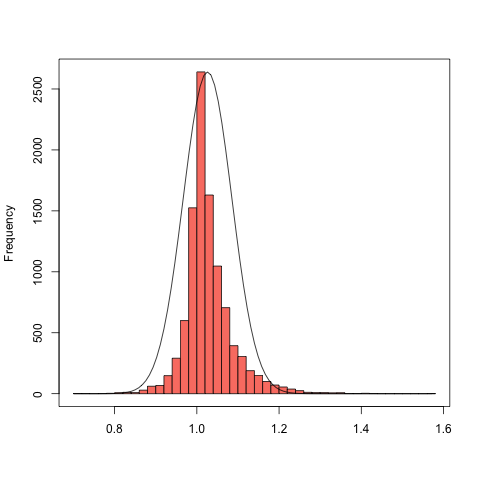
\includegraphics[width=0.48\textwidth,trim={1cm 1cm 1cm 1.5cm},clip]{../../Analysis/output/descriptives/histogram.png}
  \label{fig:APP:histogram_lambda}

  \mysubcaption{Histogram displaying the frequency distribution of $\Lambda_{i}$ over all 10,158 grid cells. Plot also shows the respective PDF of a normal distribution with mean and standard deviation matching $\Lambda_{i}$.}
  \end{figure}
  % End Figure

  % Figure Table Basic Corrs
    \begin{table}[h] \centering
      \caption{Correlations of $\Lambda_{i}$ with the Various Control Sets}
      \label{tab:APP:basic_corrs}
      \resizebox{!}{0.48\textheight}{


      \begin{tabular}{@{\extracolsep{0pt}}lccc}
      \\[-1.8ex]\hline
      \hline \\[-1.8ex]
       & \multicolumn{3}{c}{\textit{Dependent variable: $\Lambda_{i}$}} \\
      \cline{2-4}
      \\[-1.8ex] & Geo & + FE & + Simulation\\
      \hline \\[-1.8ex]
       Altitude & 0.00001 & $-$0.00001 & $-$0.00001 \\
        & (0.00001) & (0.00001) & (0.00001) \\
        & & & \\[-1.8ex]
       Average Yearly Temperature & 0.001 & $-$0.003$^{**}$ & $-$0.003$^{**}$ \\
        & (0.001) & (0.001) & (0.001) \\
        & & & \\[-1.8ex]
       Average Land Suitability & 0.008 & 0.007 & 0.007 \\
        & (0.007) & (0.007) & (0.007) \\
        & & & \\[-1.8ex]
       Malaria Transmission Index  & 0.001$^{***}$ & 0.0005$^{*}$ & 0.0005$^{*}$ \\
        & (0.0002) & (0.0003) & (0.0003) \\
        & & & \\[-1.8ex]
       Biome 1 & 0.018 & 0.022$^{**}$ & 0.022$^{*}$ \\
        & (0.020) & (0.011) & (0.011) \\
        & & & \\[-1.8ex]
       Biomes 2 \& 3 & $-$0.027 & $-$0.020 & $-$0.020 \\
        & (0.022) & (0.014) & (0.014) \\
        & & & \\[-1.8ex]
       Biome 5 & $-$0.049$^{**}$ & $-$0.036$^{**}$ & $-$0.036$^{**}$ \\
        & (0.024) & (0.016) & (0.016) \\
        & & & \\[-1.8ex]
       Biomes 7 \& 9 & 0.017 & 0.025$^{**}$ & 0.025$^{**}$ \\
        & (0.020) & (0.011) & (0.011) \\
        & & & \\[-1.8ex]
       Biome 10 & 0.015 & 0.022$^{**}$ & 0.022$^{**}$ \\
        & (0.020) & (0.011) & (0.011) \\
        & & & \\[-1.8ex]
       Biome 12 & $-$0.028$^{***}$ & $-$0.026$^{**}$ & $-$0.025$^{*}$ \\
        & (0.022) & (0.013) & (0.014) \\
        & & & \\[-1.8ex]
       Biome 13 & 0.005 & 0.009 & 0.008 \\
        & (0.020) & (0.010) & (0.011) \\
        & & & \\[-1.8ex]
       Biome 14 & $-$0.005$^{***}$ & $-$0.002 & $-$0.002 \\
        & (0.035) & (0.033) & (0.032) \\
        & & & \\[-1.8ex]
       $<25$KM to Natural Harbour & $-$0.019$^{***}$ & $-$0.017 & $-$0.014 \\
        & (0.012) & (0.012) & (0.013) \\
        & & & \\[-1.8ex]
       $<25$KM to Navigable River & $-$0.019$^{***}$ & $-$0.005 & $-$0.001 \\
        & (0.007) & (0.005) & (0.005) \\
        & & & \\[-1.8ex]
       $<25$KM to Lake & $-$0.001$^{***}$ & 0.007 & 0.006 \\
        & (0.009) & (0.009) & (0.008) \\
        & & & \\[-1.8ex]
       Yearly Growing Days & $-$0.00001 & $-$0.0001 & $-$0.0001 \\
        & (0.00003) & (0.00004) & (0.00004) \\
        & & & \\[-1.8ex]
       Average Precipitation & 0.00002$^{***}$ & 0.00005 & 0.00004 \\
        & (0.0001) & (0.0001) & (0.0001) \\
        & & & \\[-1.8ex]
       Border Cell & 0.001$^{***}$ & 0.001$^{**}$ & 0.001$^{**}$ \\
        & (0.001) & (0.001) & (0.001) \\
        & & & \\[-1.8ex]
       Longitude & 0.001$^{***}$ & $-$0.001 & $-$0.001 \\
        & (0.0003) & (0.001) & (0.001) \\
        & & & \\[-1.8ex]
       Longitude$^{2}$ & 0.00003 & $-$0.00002 & $-$0.00002 \\
        & (0.00002) & (0.00003) & (0.00003) \\
        & & & \\[-1.8ex]
       Longitude$^{3}$ & $-$0.00000$^{***}$ & 0.00000 & 0.00000 \\
        & (0.00000) & (0.00000) & (0.00000) \\
        & & & \\[-1.8ex]
       Longitude$^{4}$ & 0.00000$^{**}$ & $-$0.00000 & $-$0.00000 \\
        & (0.00000) & (0.00000) & (0.00000) \\
        & & & \\[-1.8ex]
       Latitude & $-$0.001 & $-$0.001 & $-$0.001 \\
        & (0.0003) & (0.001) & (0.001) \\
        & & & \\[-1.8ex]
       Latitude$^{2}$ & 0.00001 & 0.00001 & 0.00001 \\
        & (0.00002) & (0.00003) & (0.00003) \\
        & & & \\[-1.8ex]
       Latitude$^{3}$ & 0.00000 & 0.00000 & 0.00000 \\
        & (0.00000) & (0.00000) & (0.00000) \\
        & & & \\[-1.8ex]
       Latitude$^{4}$ & 0.000 & $-$0.000 & $-$0.000 \\
        & (0.00000) & (0.00000) & (0.00000) \\
        & & & \\[-1.8ex]
       Terrain Ruggedness &  &  & $-$0.00000 \\
        &  &  & (0.00000) \\
        & & & \\[-1.8ex]
       Average Night Lights &  &  & $-$0.001$^{***}$ \\
        &  &  & (0.0003) \\
        & & & \\[-1.8ex]
       Total Population &  &  & 0.000 \\
        &  &  & (0.000) \\
        & & & \\[-1.8ex]
       Urban Grid Cell &  &  & 0.006 \\
        &  &  & (0.003) \\
        & & & \\ [-1.8ex]
      \hline \\[-1.8ex]
      Country FE &  & Yes & Yes \\
      Observations & 10,158 & 10,158 & 10,158 \\
      R$^{2}$ & 0.062 & 0.122 & 0.124 \\
      \hline
      \hline \\[-1.8ex]
      \textit{Note:}  & \multicolumn{3}{r}{$^{*}$p$<$0.1; $^{**}$p$<$0.05; $^{***}$p$<$0.01} \\
      \end{tabular}

    }

    \mysubcaption{}
    \end{table}
    % End Figure


% Figure Table favoritism
  \begin{table}[h] \centering
    \caption{Favoritism towards Ethnic Homelands while Cutting out Birthplaces}
    \label{tab:APP:favoritism_sans}
    \resizebox{\textwidth}{!}{


    \begin{tabular}{@{\extracolsep{5pt}}lcccccccc}
    \\[-1.8ex]\hline
    \hline \\[-1.8ex]
     & \multicolumn{8}{c}{\textit{Dependent variable: Local Infrastructure Discrimination Index $\Lambda_{i}$}} \\
    \cline{2-9} \\[-1.8ex]
  & \multicolumn{5}{c}{Full Sample} & \multicolumn{3}{c}{Excluding Capitals} \\
    \cline{2-6}   \cline{7-9}
    \\[-1.8ex] & (1) & (2) & (3) & (4) & (5) & (6) & (7) & (8)\\
    \hline \\[-1.8ex]
    Years in Power & $-$0.0001 & $-$0.0002 & $-$0.0004 &  &  & $-$0.00004 & $-$0.0003 &  \\
     & (0.0003) & (0.0003) & (0.0004) &  &  & (0.0002) & (0.0003) &  \\
     & & & & & & & & \\
    Years in Power $\times$ Democracy &  &  & 0.0004 &  &  &  & 0.0005 &  \\
     &  &  & (0.0004) &  &  &  & (0.0004) &  \\
     & & & & & & & & \\
    In Power Dummy &  &  &  & $-$0.0002 & $-$0.002 &  &  & $-$0.002 \\
     &  &  &  & (0.005) & (0.005) &  &  & (0.005) \\
     & & & & & & & & \\
   \hline \\[-1.8ex]
   Country FE & Yes & Yes & Yes & Yes & Yes & Yes & Yes & Yes \\
   Geographic controls & Yes & Yes & Yes & Yes & Yes & Yes & Yes & Yes \\
   Simulation controls &  & Yes & Yes &  & Yes & Yes & Yes & Yes \\
   Observations & 926 & 926 & 926 & 926 & 926 & 890 & 890 & 890 \\
   R$^{2}$ & 0.163 & 0.167 & 0.167 & 0.163 & 0.166 & 0.176 & 0.177 & 0.176 \\
   \hline
   \hline \\[-1.8ex]
   \textit{Note:}  & \multicolumn{8}{r}{$^{*}$p$<$0.1; $^{**}$p$<$0.05; $^{***}$p$<$0.01} \\
   \end{tabular}

  }

  \mysubcaption{Replication of Table \ref{tab:favoritism}, Panel A, yet on the sample of ethnic homelands cutting out the grid cell in which a leader was born. This is to investigate whether ethnic homelands are better off when one of their members is elected to national office, beyond the effect of geographically confined birthplace favouritism. This procedure leads to the loss of six homelands, which only consist of one grid cell. Controls clusters, and data sources as in Table \ref{tab:favoritism}. Note that cutting out birthplace polygons can lead to selection bias and hence confound estimates (see text).}
  \end{table}
  % End Figure

% Figure Table AID IV

\begin{table}[!h] \centering
    \caption{Instrumental Variable Results for Foreign Aid Projects}
    \label{tab:APP:Aid_IV}
    \resizebox{\textwidth}{!}{

  \begin{tabular}{@{\extracolsep{5pt}}lcccccccc}
  \\[-1.8ex]\hline
  \hline \\[-1.8ex]
     & \multicolumn{8}{c}{\textit{Dependent variable: Local Infrastructure Discrimination Index $\Lambda_{i}$}} \\
       \cline{2-9}
  \\[-1.8ex] & (1) & (2) & (3) & (4) & (5) & (6) & (7) & (8)\\
  \hline \\[-1.8ex]
  \multicolumn{9}{l}{\textit{(a) First Stage -- aid flows regressed on presence of historical mission}} \\
  \\[-1.8ex]
  Missionary presence & 5.983$^{***}$ & 1.224$^{*}$ & 3.276$^{***}$ & 0.890$^{**}$ & 1.643$^{***}$ & 0.803$^{***}$ & 0.732$^{***}$ & 0.391$^{***}$ \\
   & (0.942) & (0.721) & (0.556) & (0.419) & (0.228) & (0.154) & (0.125) & (0.094) \\
   & & & & & & & & \\
 \\[-1.8ex]
 F Statistic & 16.868 & 70.540& 13.255 & 53.667 & 73.880 & 119.077& 63.364& 83.522\\
 \hline \\[-1.8ex]
 \\[-1.8ex]
\multicolumn{9}{l}{\textit{(b) Second Stage -- Local Infrastructure Discrimination Index $\Lambda_{i}$ regressed on predicted aid flows}} \\
\\[-1.8ex]
Total disbursements & $-$0.002$^{***}$ & $-$0.008 &  &  &  &  &  &  \\
\hspace*{3mm} in 2011 US dollars & (0.0005) & (0.005) &  &  &  &  &  &  \\
 & & & & & & & & \\
Transport-sector disbursements &  &  & $-$0.003$^{***}$ & $-$0.012$^{*}$ &  &  &  &  \\
\hspace*{3mm} in 2011 US dollars &  &  & (0.001) & (0.006) &  &  &  &  \\
 & & & & & & & & \\
Number of projects &  &  &  &  & $-$0.006$^{***}$ & $-$0.013$^{***}$ &  &  \\
 &  &  &  &  & (0.002) & (0.004) &  &  \\
 & & & & & & & & \\
Number of transport projects &  &  &  &  &  &  & $-$0.013$^{***}$ & $-$0.026$^{***}$ \\
 &  &  &  &  &  &  & (0.004) & (0.009) \\
 & & & & & & & & \\
\hline \\[-1.8ex]
Country FE & Yes & Yes & Yes & Yes & Yes & Yes & Yes & Yes \\
Geographic controls & Yes & Yes & Yes & Yes & Yes & Yes & Yes & Yes \\
Simulation controls &  & Yes &  & Yes &  & Yes &  & Yes \\
Observations & 10,158 & 10,158 & 10,158 & 10,158 & 10,158 & 10,158 & 10,158 & 10,158 \\
 \hline
 \hline \\[-1.8ex]
 \textit{Note:}  & \multicolumn{8}{r}{$^{*}$p$<$0.1; $^{**}$p$<$0.05; $^{***}$p$<$0.01} \\
 \end{tabular}


}

\mysubcaption{Two staged least squares instrumental regressions replicating the cross-sectional findings from Table \ref{tab:Aid_Baseline}. Empirical strategy follows \cite{Castello-Climent_HigherEducationProsperity_2017}. Panel (a) regresses World Bank aid variables on an indicator equalling one if a grid cell was home to a historical Catholic or Protestant missionary. Panel (b) regresses $\Lambda_{i}$ on predicted values from the first stage. Controls, clusters, and aid data as in Table \ref{tab:Aid_Baseline}. All estimations also additionally control for the presence of colonial railways (in total kilometres) as proposed by \citeauthor{Castello-Climent_HigherEducationProsperity_2017}. Missionary data from \cite{Nunn_ReligiousConversionColonial_2010}. Link between historical missions and current aid flows first investigated by \cite{Alpino_LightingPathInfluence_2017}.}
\end{table}
% End Figure

% Figure Table Old Projects
\begin{table}[h] \centering
  \caption{15+ year old Projects}
  \label{tab:APP:old_projects}
  \resizebox{\textwidth}{!}{


  \begin{tabular}{@{\extracolsep{5pt}}lcccccccc}
  \\[-1.8ex]\hline
  \hline \\[-1.8ex]
   & \multicolumn{8}{c}{\textit{Dependent variable: Local Infrastructure Discrimination Index $\Lambda_{i}$}} \\
  \cline{2-9}
  \\[-1.8ex] & (1) & (2) & (3) & (4) & (5) & (6) & (7) & (8)\\
  \hline \\[-1.8ex]
  Total disbursements & $-$0.001$^{*}$ & $-$0.001$^{*}$ &  &  &  &  &  &  \\
   \hspace*{3mm} pre-2002 in 2011 US dollars & (0.0004) & (0.0004) &  &  &  &  &  &  \\
   & & & & & & & & \\
  Transport-sector disbursements &  &  & 0.0005 & 0.001 &  &  &  &  \\
   \hspace*{3mm} pre-2002 in 2011 US dollars &  &  & (0.001) & (0.001) &  &  &  &  \\
   & & & & & & & & \\
  Number of projects &  &  &  &  & $-$0.004$^{***}$ & $-$0.005$^{***}$ &  &  \\
   \hspace*{3mm} pre-2002 &  &  &  &  & (0.001) & (0.001) &  &  \\
   & & & & & & & & \\
  Number of transport projects &  &  &  &  &  &  & $-$0.003$^{***}$ & $-$0.003$^{***}$ \\
   \hspace*{3mm} pre-2002 &  &  &  &  &  &  & (0.001) & (0.001) \\
   & & & & & & & & \\
 \hline \\[-1.8ex]
 Country FE & Yes & Yes & Yes & Yes & Yes & Yes & Yes & Yes \\
 Geographic controls & Yes & Yes & Yes & Yes & Yes & Yes & Yes & Yes \\
 Simulation controls &  & Yes &  & Yes &  & Yes &  & Yes \\
 Observations & 10,158 & 10,158 & 10,158 & 10,158 & 10,158 & 10,158 & 10,158 & 10,158 \\
 R$^{2}$ & 0.122 & 0.124 & 0.122 & 0.124 & 0.123 & 0.125 & 0.122 & 0.124 \\
 \hline
 \hline \\[-1.8ex]
 \textit{Note:}  & \multicolumn{8}{r}{$^{*}$p$<$0.1; $^{**}$p$<$0.05; $^{***}$p$<$0.01} \\
 \end{tabular}

}

\mysubcaption{Replication of Table \ref{tab:Aid_Baseline}, Panel A, yet only examining projects completed before 2002. Controls, clusters, and data as in Table \ref{tab:Aid_Baseline}.}
\end{table}
% End Figure

\end{spacing}

\end{document}
